% !Mode:: "TeX:UTF-8"
%!TEX program  = xelatex
% ============================================================
% 2026 年中国研究生数学建模竞赛 E 题论文
% 题目：复杂场景下多模态情感预测的数学建模与算法设计
% 版式由 gmcmthesis.cls 提供，本文件负责内容组织与门禁标签。
% 编译方式：XeLaTeX。
% ============================================================
\documentclass[bwprint]{gmcmthesis}

\hypersetup{hidelinks, allcolors=black}

\usepackage{subfig}
\usepackage{siunitx}
\usepackage{needspace}

% 图片按项目根目录解析：先查模板 figures/，再查论文目录与项目根目录
\graphicspath{{figures/}{./}{../}}

% 图/表全篇连续编号：取消 figure/table 对 section 的计数从属，
% 保持 class 可替换可升级；equation 编号保持 class 原有章节编号不变。
\counterwithout{figure}{section}
\counterwithout{table}{section}

% 算法
\usepackage[noend]{algpseudocode}
\usepackage{algorithmicx,algorithm}
\floatname{algorithm}{算法}
\renewcommand{\algorithmicrequire}{\textbf{输入:}}
\renewcommand{\algorithmicensure}{\textbf{输出:}}

% 引用以上标数字角标显示
\makeatletter
\def\@cite#1#2{\textsuperscript{[{#1\if@tempswa , #2\fi}]}}
\makeatother

%===================== 建模论文题目与封面信息 =====================

\title{复杂场景下多模态情感预测的数学建模与算法设计}
\baominghao{\hspace{6em} 20260900001}
\schoolname{\hspace{5.8em} 学校名称填写}
\membera{\hspace{6em} 成员A}
\memberb{\hspace{6em} 成员B}
\memberc{\hspace{6em} 成员C}

%=======================================================

\begin{document}
\label{body:start}

%生成封面（模板规定动作，不得删除）
\maketitle

\begin{abstract}\label{abstract:start}
多模态情感预测是具身智能与自然人机交互的基础支撑技术。真实交互中情绪通过文本语义、语音韵律与面部表情
协同表达，而三类信号在采样频率、特征维度与时间尺度上差异显著；实际采集又常因画面遮挡、环境噪声与转写
失败造成局部时段模态不可用，多数模型还只能给出结果而难以追溯判断依据。本文以赛题提供的 CMU-MOSEI 系列
数据为唯一数据来源，围绕多模态特征提取与时序对齐、模态缺失条件下的鲁棒预测、可解释性情感预测三个层级
建立统一的数学建模与算法框架。全文共用同一套三模态时序特征接口与同一套评价口径，参数只在附件2 训练集上
学习，模型结构与决策阈值在验证集上选择，附件3 与附件4 只用于最终推理。

\textbf{针对问题一}，本文把原始视频片段映射到统一时间栅格，定义时间量化算子与区间聚合规则，得到文本
768 维、语音 74 维、视觉 35 维、50 个序列位置的三模态特征矩阵。100 条样本全部完成提取，无效数值计数为 0，
语音有效位置均值 49.69、视觉 33.97，对齐粒度介于 0.0451 与 0.5858 秒之间；典型样本的文本词元落位、
语音帧级能量与视觉帧间灰度差在同一条时间轴上彼此对应，说明对齐规则把三模态放到了同一时间尺度。

\textbf{针对问题二}，本文提出可信度门控与跨模态注意力相结合的鲁棒融合模型，门控由编码内容、可用性掩码
与模态嵌入共同决定，并与掩码相乘形成硬约束，缺失位置的权重恒为零。验证集上情感强度平均绝对误差为
0.6418、极性准确率为 0.5632；去掉门控后误差升至 0.6480，去掉跨模态注意力后升至 0.6448，仅用文本为
0.6616，仅用语音与仅用视觉分别为 0.9479 与 0.9168。缺失率升到 0.7 时全模态缺失误差从 0.6418 升到
0.6674，仅缺失文本时升到 0.6649，而仅缺失语音与仅缺失视觉的误差几乎不变。附件3 的 30 条样本给出
1 条负向、9 条中性、20 条正向。

\textbf{针对问题三}，本文把融合过程分解为模态作用程度、位置重要性与逐位置模态贡献三层可读量，并用
删除实验做外部核对。删除前 10 个关键位置引起的预测值偏移为 0.0909，同规模随机位置为 0.0206，定位增益
\textbf{0.0703} 并随删除规模单调增大。验证集模态作用程度为文本 0.3820、语音 0.3142、视觉 0.3038；语音与视觉
证据高度集中在序列前段，文本证据贯穿全程。附件4 的 20 条样本中 19 条以文本为主要参考模态。

本文把缺失掩码同时用作门控的硬约束与解释权重分解的依据，使鲁棒性与可解释性共享同一套结构，并给出
可复算的定位增益指标。模型的边界在于语音与视觉编码器自身性能较弱，以及附件3、附件4 的特征分布与训练集
不完全一致，这两点在正文中逐项说明。
\keywords{多模态情感预测\quad 时序对齐\quad 缺失模态鲁棒建模\quad 注意力归因\quad 证据定位}\label{abstract:end}

\end{abstract}

\pagestyle{plain}

\maketoc
\clearpage

% ============================================================
% 正文
% ============================================================

\section{问题重述}

\subsection{问题背景}

情感分析是具身智能、自然人机交互与在线内容理解的关键支撑技术。真实交互中的情绪并不只通过单一通道
表达：说话人用词的选择携带语义极性，语调、节奏与停顿携带韵律强度，面部表情与头部姿态携带即时的情绪
波动。三类信号在采样频率、特征维度与时间尺度上差异显著，文本以词为粒度、语音以毫秒级帧为粒度、
视觉以帧为粒度，把它们联合建模并落到同一条时间轴上，是提升复杂场景下情绪理解准确性与稳定性的核心路径。

工程落地还面临两类现实约束。其一是局部时段模态信息不可用：摄像头被遮挡时视觉通道在该时段没有有效内容，
环境噪声使语音识别置信度骤降，转写失败使文本片段缺失。这类缺失是局部连续的区间缺失，而不是整段模态
消失，常规固定权重融合模型在这种条件下性能急剧下降。其二是可信性约束：多数模型只输出一个预测值，
决策依据无法追溯与复核，在需要人机协同判断的场景中难以被接受。

本题以 CMU-MOSEI 英文多模态情感数据集为基础，围绕多模态特征提取与时序对齐、模态缺失条件下的鲁棒预测、
可解释性情感预测三个层级开展系统性建模研究。赛题明确规定，所有建模任务以赛题提供的 CMU-MOSEI 系列数据
为唯一数据来源，不得引入其他公开或私有情感数据集参与训练、微调、参数优化、阈值选择或结果统计；允许使用
开源特征提取工具与预训练模型，但须标注名称、版本与核心参数。本项目严格执行该约束，全文未引入任何外部
数据集与外部预训练权重。

\subsection{问题提出}

赛题依次提出三项建模任务，其输入、输出与约束如表~\ref{tab:problem} 所示。

\begin{table}[htp!]
\centering
\caption{三项建模任务的输入、输出与主要约束}
\label{tab:problem}
\renewcommand\arraystretch{1.25}
\begin{tabular}{|p{1.5cm}|p{3.3cm}|p{3.5cm}|p{5.2cm}|}
\hline
任务 & 输入 & 输出 & 主要约束 \\
\hline
问题一 & 附件1 的 100 条原始视频与转写标注 &
三模态时序特征文件、对齐规则、全量结果汇总表 &
样本一一对应；序列位置与有效长度可核验；方法与参数可复现 \\
\hline
问题二 & 附件2 对齐版特征（训练/验证）与附件3 无标签专项测试集 &
情感极性与强度预测、缺失类型/位置/时长的影响规律 &
参数只在训练集学习；结构、超参数与阈值在验证集选择；附件3 只用于推理 \\
\hline
问题三 & 附件2 对齐版特征与附件4 完整三模态样本（含原始视频） &
情感极性与强度预测、模态作用程度、关键证据定位 &
关键证据须可对应到原始文本片段、语音时段或视觉关键帧 \\
\hline
\end{tabular}
\end{table}

三项任务共享同一套特征接口与评价口径。分类任务采用准确率与 F1 值评价，回归任务采用平均绝对误差与
皮尔逊相关系数评价。本文的技术路线如图~\ref{fig:roadmap} 所示，三个层级依次解决“特征与对齐是否可靠”、
“缺失条件下是否稳定”、“判断依据是否可复核”，上层结论直接依赖下层的输出质量。

\begin{figure}[htp!]
\centering

\includegraphics[width=0.96\textwidth]{手绘图/技术路线图.png}
\caption{三阶段递进式建模技术路线图}
\label{fig:roadmap}
\end{figure}

该图把全文的建模主线拆成三层：第一层完成三模态特征提取与统一时间栅格对齐，输出三模态时序特征矩阵；
第二层在缺失掩码约束下做可信度门控与跨模态注意力融合，输出情感极性与情感强度；第三层把融合权重分解为
模态作用程度、位置重要性与逐位置模态贡献，输出可复核的解释结论。层间的依赖关系是单向的，对齐质量决定
鲁棒模型可用的输入，鲁棒模型输出的时序权重决定可解释性分析的对象。图的提示词与生成参数保存在
手绘图/技术路线图提示词.md，便于复核。

\section{模型假设与符号说明}

\subsection{模型假设}

\begin{enumerate}
\item 每条视频片段的情感标注在片段内部恒定，即整段共享同一个连续情感强度与极性标签。附件2 的标注确实
以片段为单位给出，该假设与数据组织方式一致。
\item 片段的物理时间轴可由容器时长可靠读出，文本、语音与视觉三模态共享同一条时间轴，模态之间不存在
系统性的时钟偏移。附件2 的对齐版特征已按统一位置组织，该假设与其存储口径一致。
\item 缺少逐词时间戳时，语音与视觉的局部特征按时间比例映射到统一栅格，单栅格的时间分辨率误差不超过
一个栅格宽度。附件1 只提供整句转写与视频文件，该假设是唯一可行的对齐口径。
\item 文本通道按词元在句中的出现次序均匀分配到统一位置，位置 $k$ 覆盖词元区间
$[\lfloor kT/L\rfloor,\lfloor (k+1)T/L\rfloor)$；区间为空时取相邻词元，因此文本通道的全部位置均有效。
该组织方式只影响文本特征的时间权重分布，不改变整句语义的完整性。
\item 缺失表现为序列上连续区间的特征值全零，缺失区间的位置与长度可以从数值本身反演，不需要额外的
掩码文件。附件3 的数据形式与该假设一致。
\item 训练集的缺失模式与专项测试集同源，可以用训练集上随机施加的缺失区间近似专项测试集的缺失分布。
该假设用于规律分析与增强策略比较，其偏差在结果解释中说明。
\item 缺失区间内的信息确实不可用，禁止用插值、外推或跨样本复制来补全缺失值参与预测；模型只能依据
可用位置与掩码本身作推断。
\item 语音与视觉可能在同一时段同时缺失，缺失事件不假定相互独立。附件3 的实际掩码支持这一判断。
\end{enumerate}

\needspace{16\baselineskip}
\subsection{符号说明}

全文符号统一如表~\ref{tab:symbol} 所示。下标 $i$ 表示样本、$k$ 表示序列位置、$m$ 表示模态；
上标只用于区分模态，不表示幂次。

\renewcommand\arraystretch{1.2}
\newcolumntype{L}{>{\quad}X}
\newcolumntype{P}[1]{>{\centering\arraybackslash}p{#1}}
\noindent\begin{tabular}{|p{2.4cm}|p{11.4cm}|}
  \hline
  符号    &   \quad 意义 \\
  \hline
  $n$ & 样本总数；附件1 中 $n=100$ \\
  \hline
  $L$ & 统一序列位置数，$L=50$ \\
  \hline
  $m$ & 模态标识，$m\in\{\mathrm{txt},\mathrm{aud},\mathrm{vis}\}$ \\
  \hline
  $D_i$ & 第 $i$ 条片段的时长（秒） \\
  \hline
  $\tau_k$ & 第 $k$ 个序列位置的代表时刻，$\tau_k=(k+0.5)D_i/L$ \\
  \hline
  $I_k$ & 第 $k$ 个位置对应的时间区间 $[kD_i/L,(k+1)D_i/L)$ \\
  \hline
  $\kappa(t)$ & 时间量化算子，把物理时刻映射到栅格位置 \\
  \hline
  $\mathbf{x}^{m}_{i,k}$ & 第 $i$ 个样本第 $m$ 模态第 $k$ 个位置的特征向量 \\
  \hline
  $d^{m}$ & 第 $m$ 模态的特征维度；文本 768、语音 74、视觉 35 \\
  \hline
  $\mathbf{h}^{m}_{i,k}$ & 第 $m$ 模态第 $k$ 个位置的时序编码表示 \\
  \hline
  $s^{m}_{i,k}$ & 可用性掩码，1 表示该位置可用、0 表示缺失 \\
  \hline
  $g^{m}_{i,k}$ & 可信度门控权重 \\
  \hline
  $\alpha^{m}_i$ & 第 $m$ 模态在当前样本中的作用程度 \\
  \hline
  $\beta_{i,k}$ & 第 $k$ 个位置的重要性 \\
  \hline
  $c^{m}_{i,k}$ & 第 $m$ 模态在第 $k$ 个位置对判断的贡献 \\
  \hline
  $\mathcal{T}_i(K)$ & 第 $i$ 个样本重要性最高的前 $K$ 个位置集合 \\
  \hline
  $\mathbf{z}_i$ & 融合后的样本级表示 \\
  \hline
  $y^{\mathrm{cls}}_i$ & 情感极性标签，取值负向、中性、正向 \\
  \hline
  $y^{\mathrm{reg}}_i$ & 连续情感强度标注，取值区间 $[-3,3]$ \\
  \hline
  $\rho$ & 缺失率，缺失位置数占总位置数的比例 \\
  \hline
  $w_c$ & 第 $c$ 类的类别权重 \\
  \hline
  $\lambda$ & 回归项在总损失中的权重 \\
  \hline
\end{tabular}

\section{问题一模型建立与求解}

\subsection{数据预处理与探索性分析}

附件1 共 100 条样本、37 个视频标识，片段时长介于 2.257 与 29.288 秒之间，均值 7.875 秒、中位数
6.722 秒，转写文本平均 19.32 个英文词，词数范围 5 至 65。标注分布为正向 57 条、中性 25 条、负向 18 条。
附件2 共 4850 条样本，训练 3395 条、验证 728 条、测试 727 条；训练集连续情感强度均值 0.166、标准差
1.115、偏度 $-0.322$，三分类计数为负向 967、中性 758、正向 1670，中性类占比 22.3\%，存在明显类别
不平衡。数据总览如图~\ref{fig:eda1} 所示。

\begin{figure}[htp!]
\centering
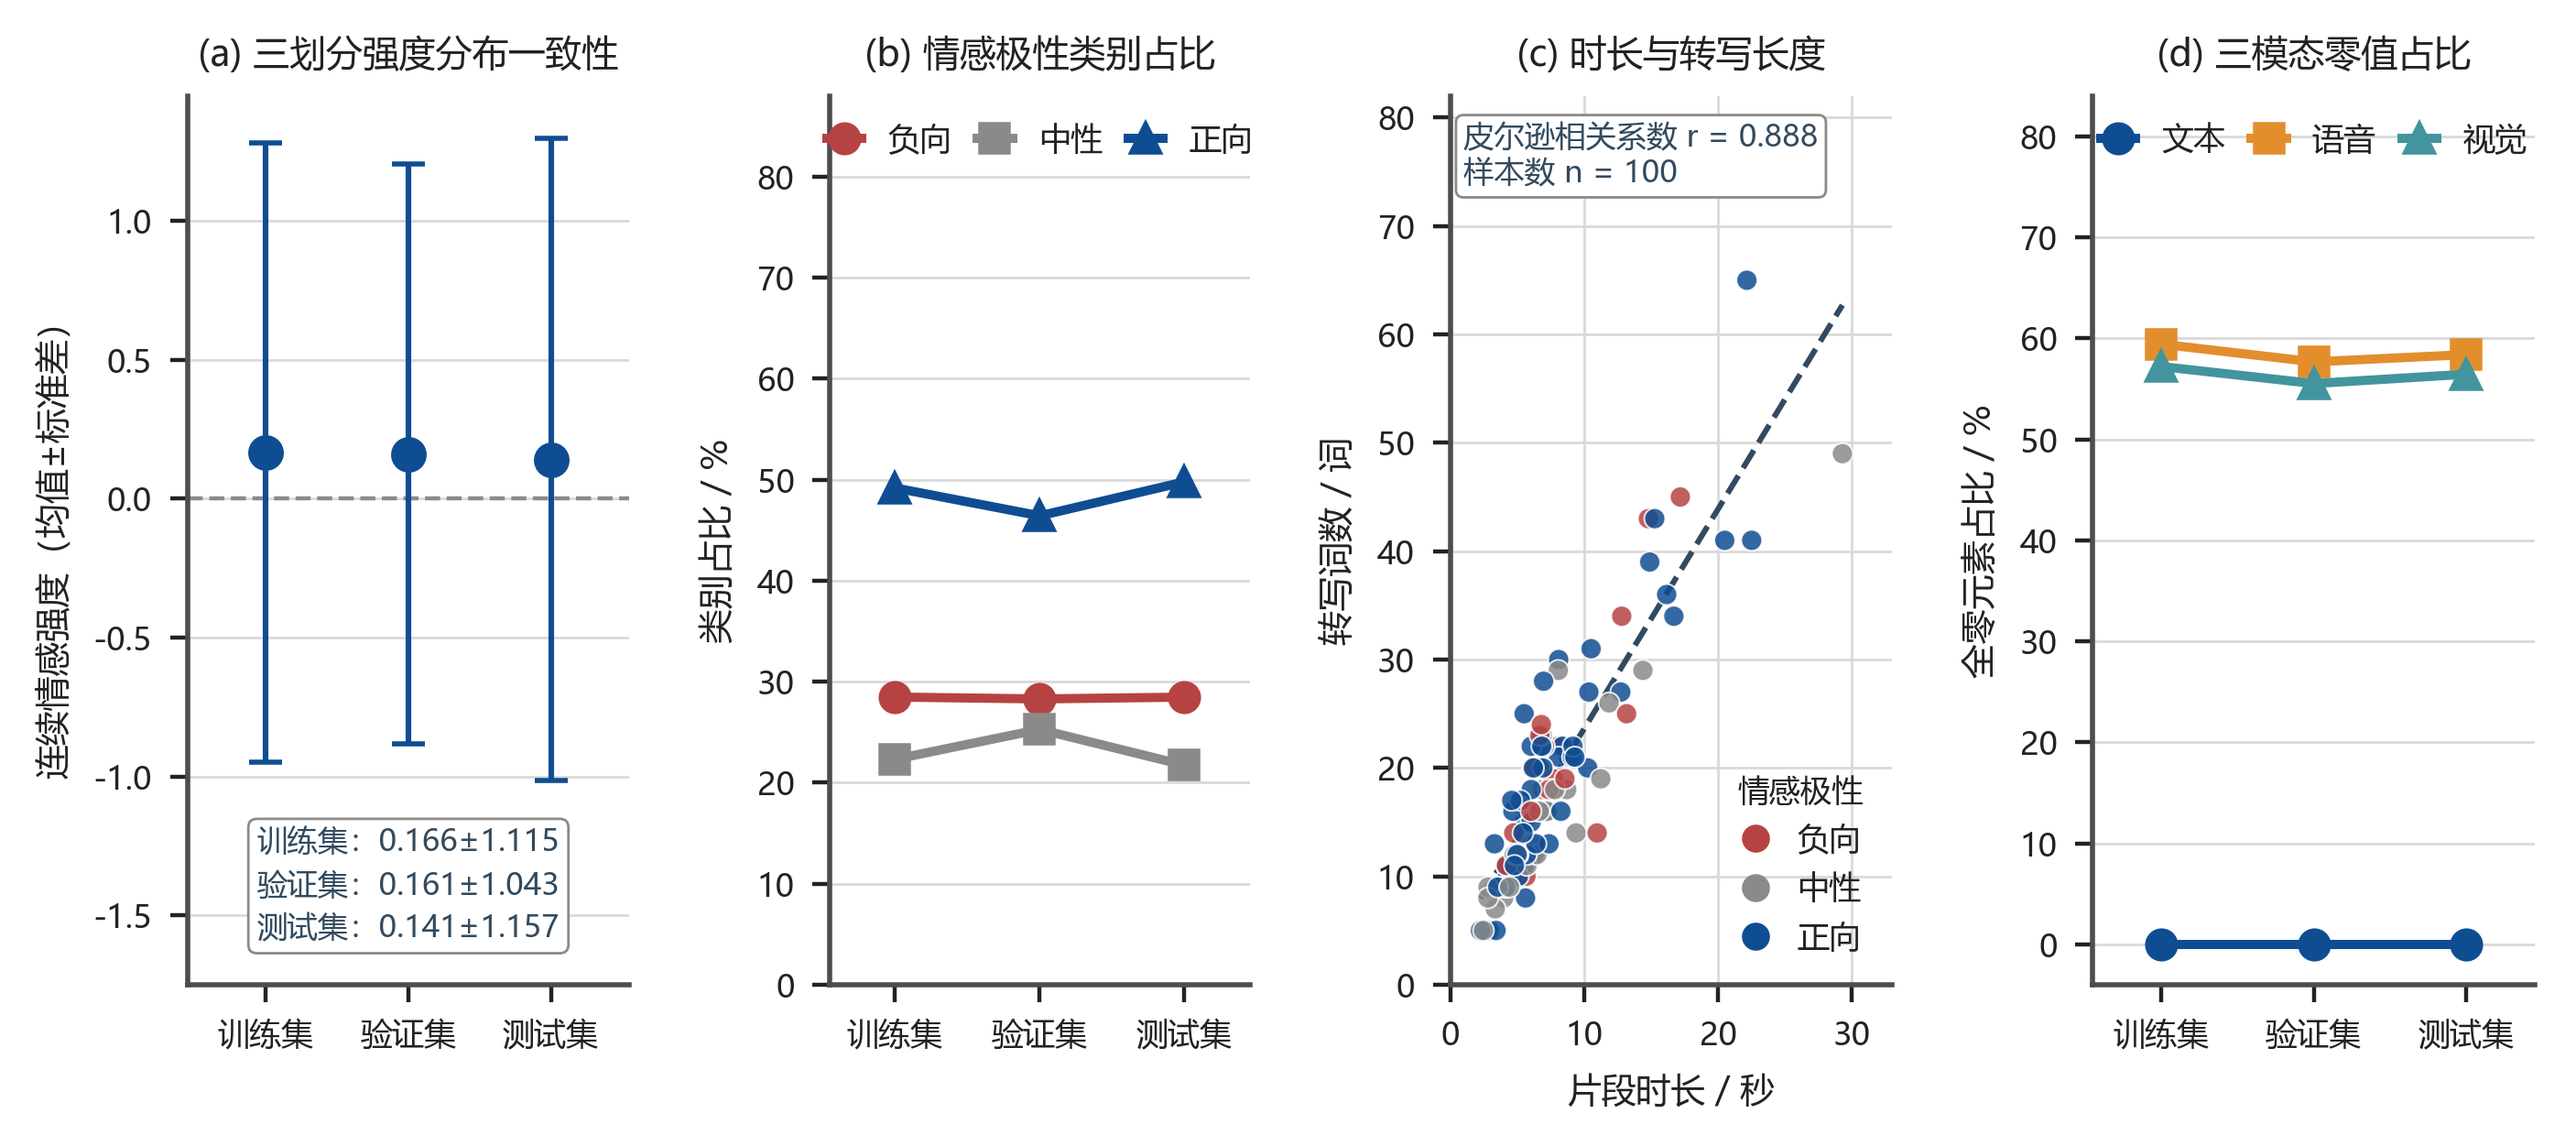
\includegraphics[width=0.99\textwidth]{figures/fig01_data_overview.png}
\caption{数据规模、标签分布、片段特征与三模态零值占比总览}
\label{fig:eda1}
\end{figure}

四个面板共同回答“数据能不能直接用于建模”。三个划分的情感强度均值分别为 0.166、0.161 与 0.141，
标准差分别为 1.115、1.043 与 1.157，分布一致性满足按划分训练与验证的前提；类别占比在三个划分中稳定在
正向约 46\% 至 50\%、负向约 28.5\%、中性约 22\% 至 25\%，因此类别不平衡是数据固有属性而非划分偏差；
片段时长与转写词数的皮尔逊相关系数为 0.888，说明转写长度随时长线性增长，为按位置等分词元提供了依据；
语音与视觉的全零元素占比稳定在 55\% 至 59\%，文本为零，说明前两个模态存在大量无效位置，而文本通道
在存储上被完整填充。

进一步的相关结构如图~\ref{fig:eda2} 所示。三模态样本级均值特征之间的相关系数为文本–语音 $-0.682$、
文本–视觉 $0.557$、语音–视觉 $-0.608$，属于中等强度；而三模态均值与情感强度的线性相关分别为
$-0.013$、$0.102$ 与 $-0.054$，全部落在弱相关带内。这一对照说明情感信息主要存在于时序局部结构而不是
全局均值，直接决定了后续必须使用时序编码而不是全局池化。

\begin{figure}[htp!]
\centering
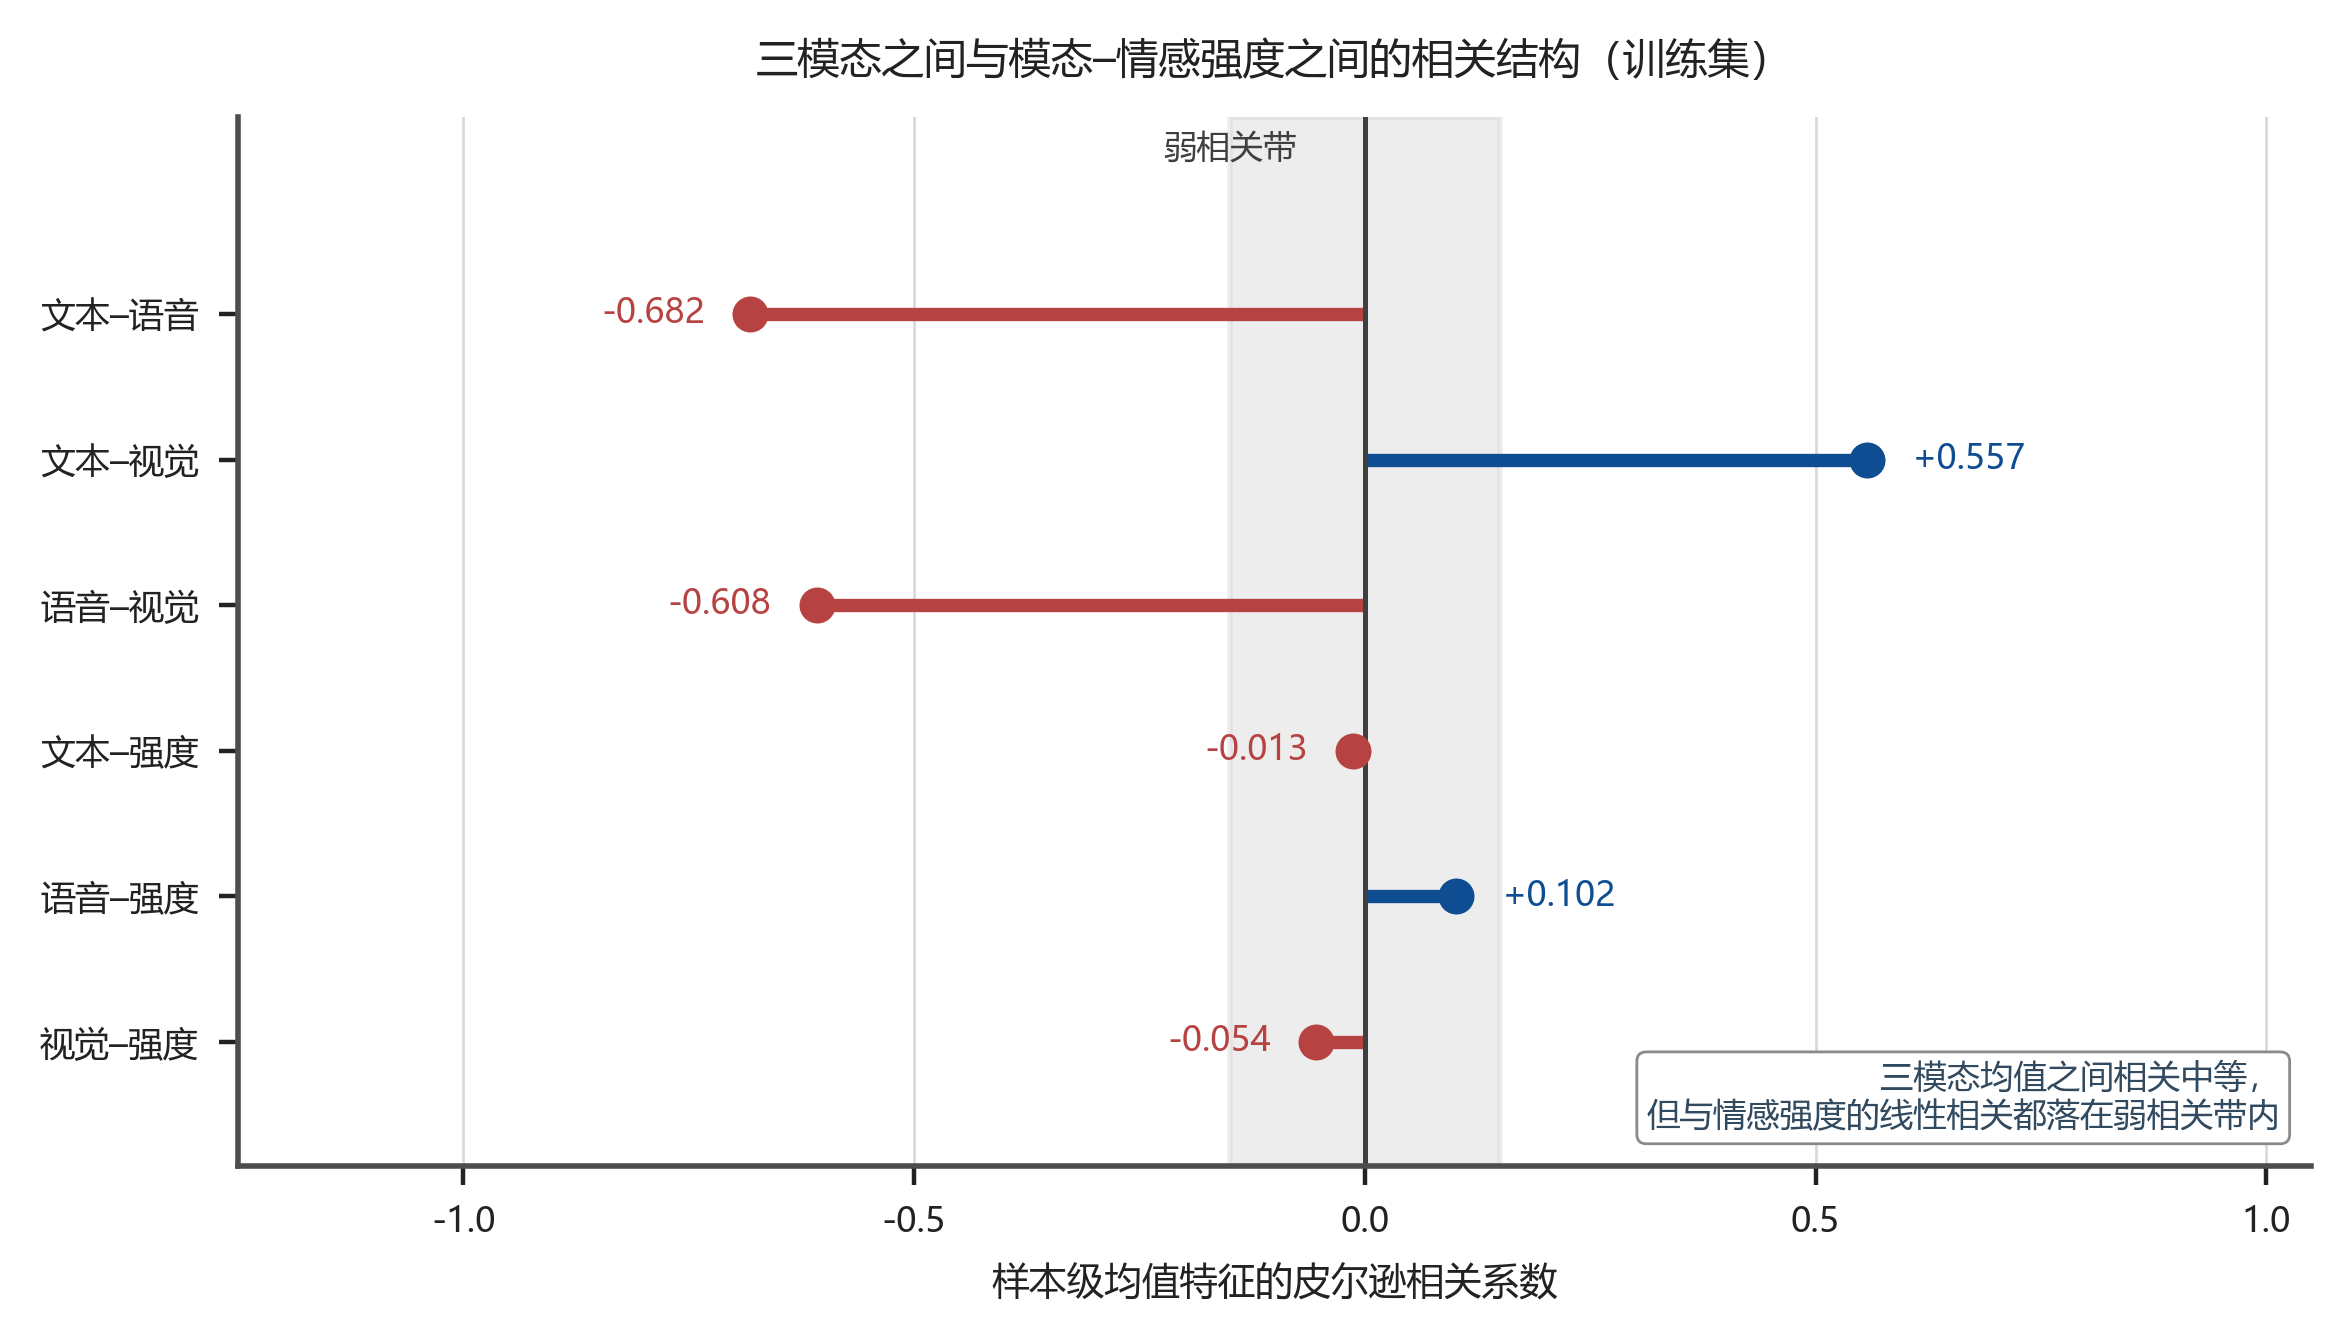
\includegraphics[width=0.82\textwidth]{figures/fig02_modality_correlation.png}
\caption{三模态之间与模态–情感强度之间的相关结构}
\label{fig:eda2}
\end{figure}

数据清洗规则如下，全部处理行为记录在数据预处理说明中：标注表只做 xlsx 到 csv 的无损格式转换；
媒体清点只读取容器元数据，不改写文件；语音第 0 维量纲为 0 至 500，与其余维度相差三个数量级，
标准化前先做符号对数压缩；附件3 的缺失掩码按“某序列位置在所有特征维度上取值全为 0”反演，位置 0 在
附件2 与附件3 的语音与视觉序列中同样恒为全零，按文件规则记为填充位而不计入缺失区间；全部原始样本
保持只读，不做替换、增补、删除或修改。

\subsection{三模态特征定义与提取}

从原始素材到标准化时序特征的完整流程如图~\ref{fig:flow} 所示。三条通道并行完成模态内特征化，
再在同一时间轴上按等分区间聚合为固定长度序列，最后登记有效长度与填充位置。

\begin{figure}[htp!]
\centering
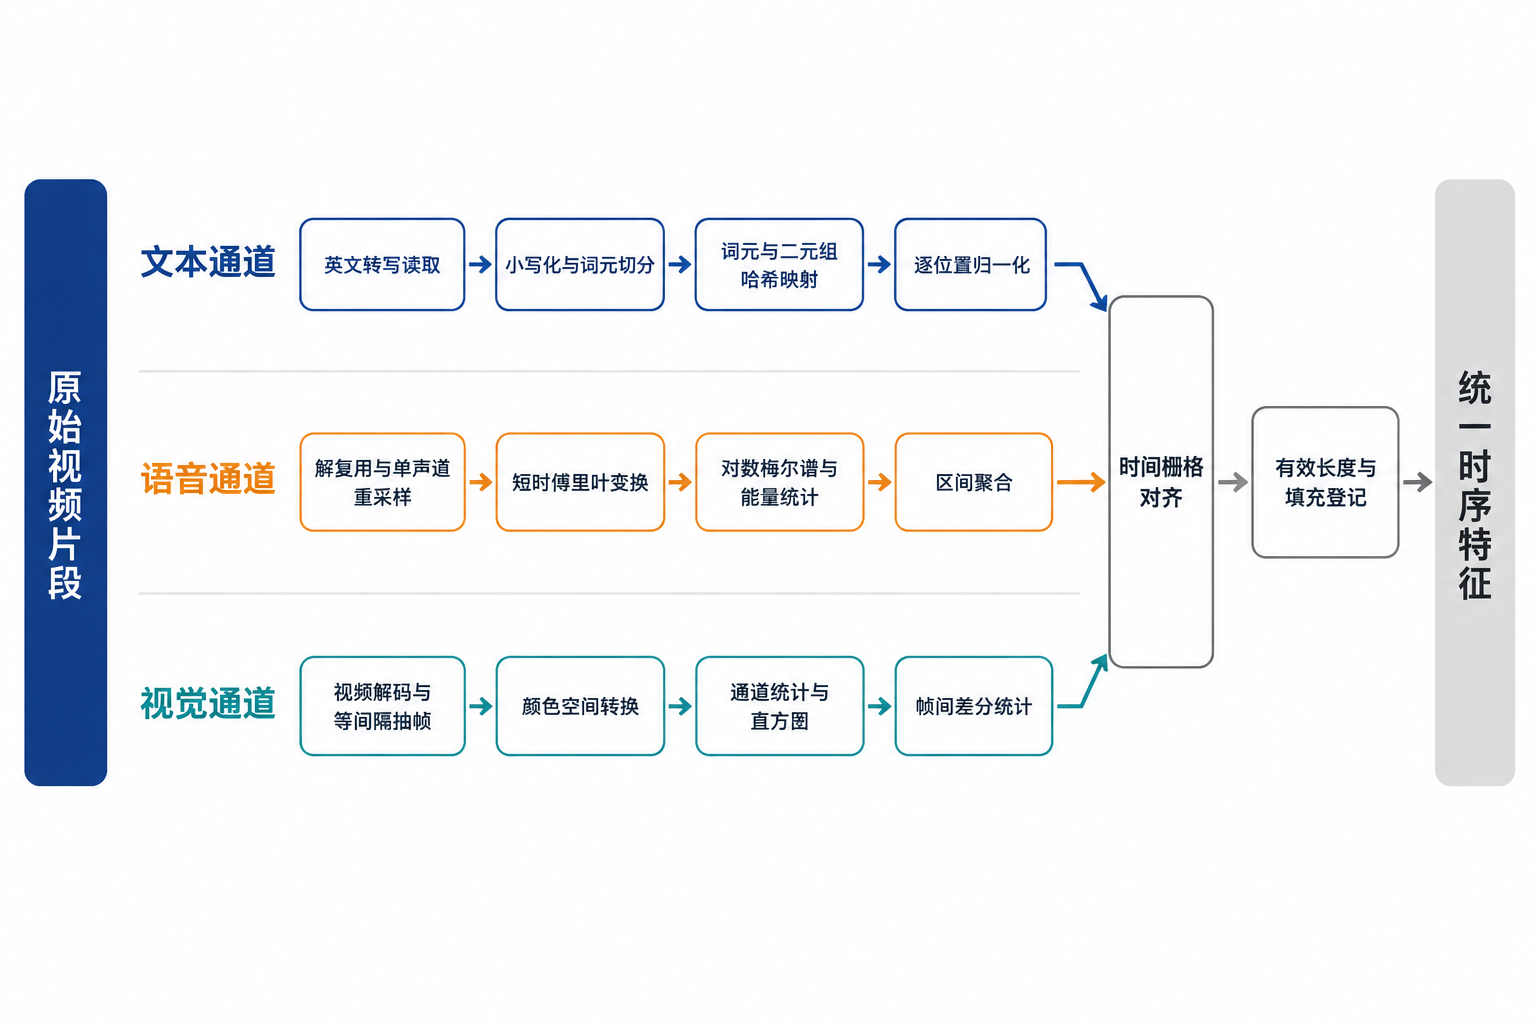
\includegraphics[width=0.96\textwidth]{手绘图/特征提取流程图.png}
\caption{三模态特征提取与时序对齐流程图}
\label{fig:flow}
\end{figure}

该图把处理链拆成“输入条带、三条模态泳道、对齐与登记、输出条带”四段。文本泳道完成转写读取、小写化
与词元切分、词元与二元组哈希映射、逐位置归一化；语音泳道完成解复用与单声道重采样、短时傅里叶变换、
对数梅尔谱与能量统计、区间聚合；视觉泳道完成视频解码与等间隔抽帧、颜色空间转换、通道统计与直方图、
帧间差分统计。三条泳道的输出汇聚到“时间栅格对齐”与“有效长度与填充登记”两个环节，对应下文的时间
量化算子与有效标志定义。图的提示词保存在手绘图/特征提取流程图提示词.md。

\textbf{语音特征}的构造如下：用 ffmpeg 把视频解复用为 16 kHz 单声道 PCM，用 librosa 计算对数梅尔谱与帧级
均方根能量，窗长 400 采样点、帧移 160 采样点、梅尔带数 64、频率范围 20 Hz 至 8 kHz。第 $k$ 个位置的
特征向量由四段拼接而成：前 64 维为落入区间 $I_k$ 的所有帧在 64 个梅尔带上的对数功率均值；第 65 至
72 维为最低 8 个梅尔带的对数功率标准差；第 73 维为该区间内帧级均方根能量的均值；第 74 维为其标准差。

\textbf{视觉特征}的构造如下：用 ffmpeg 按 5 帧/秒抽帧并缩放到 $112\times112$，用 OpenCV 计算帧级统计量。
第 1 至 6 维为 HSV 三通道的均值与标准差；第 7 至 14 维为 8 段色调直方图均值；第 15 维为色调熵；
第 16 至 23 维为饱和度直方图均值；第 24 至 31 维为亮度直方图均值；第 32 至 33 维为相邻帧灰度差的
均值与最大值；第 34 至 35 维为灰度均值与标准差。

\textbf{文本特征}的构造如下：把转写文本小写化并做英文词元切分，把每个词元与其相邻二元组经 BLAKE2b 哈希映射到
768 维词袋，词元权重为 1.0、二元组权重为 0.5，再对每个位置做 L2 归一化。赛题允许使用开源预训练模型，
本文为满足“不引入外部数据集与外部预训练权重”的自设约束并保证离线可复现，选择哈希词袋路线；其代价是
丢失上下文语义，该代价在模型局限中明确写出。

\subsection{跨模态时序对齐模型}

\textbf{时间量化算子}的构造如下：把片段时长 $D_i$ 等分为 $L$ 个半开区间，定义把物理时刻映射到栅格位置的算子

\begin{equation}
\kappa(t)=\min\Big(L-1,\ \Big\lfloor \frac{t\,L}{D_i}\Big\rfloor\Big),
\qquad t\in[0,D_i],
\label{eq:kappa}
\end{equation}

区间 $I_k$ 是 $\kappa(t)=k$ 的原像，位置代表时刻取区间中点 $\tau_k=(k+0.5)D_i/L$。该算子的作用是
把三种不同采样频率的信号压到同一个离散时间索引上，使“同一位置”在不同模态中指向同一段真实时间。

\textbf{区间聚合}的构造如下：语音与视觉的局部特征对 $I_k$ 内的所有帧取统计聚合。以语音为例，记第 $j$ 帧的
64 维对数梅尔谱为 $\boldsymbol{\ell}_j$、帧级均方根能量为 $e_j$，$\mathcal{A}_k$ 为落入 $I_k$ 的帧集合，
则

\begin{equation}
\mathbf{x}^{\mathrm{aud}}_{i,k}=
\Big[\ \operatorname{mean}_{j\in\mathcal{A}_k}\boldsymbol{\ell}_j\ \Big\|\
\operatorname{std}_{j\in\mathcal{A}_k}\boldsymbol{\ell}^{(1:8)}_j\ \Big\|\
\operatorname{mean}_{j\in\mathcal{A}_k} e_j\ \Big\|\
\operatorname{std}_{j\in\mathcal{A}_k} e_j\ \Big],
\label{eq:audio}
\end{equation}

其中 $\boldsymbol{\ell}^{(1:8)}_j$ 表示取最低 8 个梅尔带。视觉特征对同一区间内的解码帧取 HSV 统计量、
色调熵与相邻帧灰度差统计，聚合方式与式~\eqref{eq:audio} 同构。文本特征按词元次序分块后做哈希词袋
表示并逐位置 L2 归一化。

\textbf{有效标志与填充规则}的构造如下：定义模态有效标志

\begin{equation}
m^{\mathrm{mod}}_{i,k}=\mathbb{1}\big[\mathcal{A}^{\mathrm{mod}}_{i,k}\neq\varnothing\big],
\qquad
\sum_{k=0}^{L-1} m^{\mathrm{mod}}_{i,k}\le L,
\label{eq:valid}
\end{equation}

即只有区间内确实取到帧的位置才标记为有效。该定义的作用是把“该位置是否有真实信息”与“该位置在矩阵中
是否被填充”分开：无帧位置保留为零向量并在有效标志中记为 0，不参与后续任何融合与聚合。

\textbf{约束条件}的构造如下：一是样本覆盖约束：100 条样本必须一一对应，任何样本不得被丢弃或替换；
二是时序可核验约束：位置代表时刻严格单调，$\tau_0<\tau_1<\cdots<\tau_{L-1}$，相邻间隔恒为 $D_i/L$；
三是数值约束：输出特征不得含无效数值；四是维度约束：三模态维度固定为 768、74 与 35，与附件2 的存储
口径一致。

\subsection{全量结果与典型样本核验}

\textbf{全量结果}的构造如下：100 条样本全部完成特征提取，覆盖完整性核对通过。文本、语音与视觉的特征维度分别为
768、74 与 35，序列位置数均为 50，无效数值计数为 0，片段时长范围为 2.257 至 29.288 秒。文本通道 50 个
位置全部有效，语音通道有效位置均值为 49.69，视觉通道有效位置均值为 33.97，最少 0 个、最多 48 个。
对齐粒度等于片段时长除以 50，范围为 0.0451 至 0.5858 秒。全量汇总表按样本编号与模态类型逐行登记
原始有效时长、特征维度、序列位置数、有效位置数、对齐粒度与填充位置数，共 300 行。

视觉通道的有效位置覆盖如图~\ref{fig:q1cov} 所示，横轴为序列位置，纵轴为按极性、时长排序的样本序号，
蓝色为有效、灰色为填充，红色虚线分隔三个极性区间。

\begin{figure}[htp!]
\centering
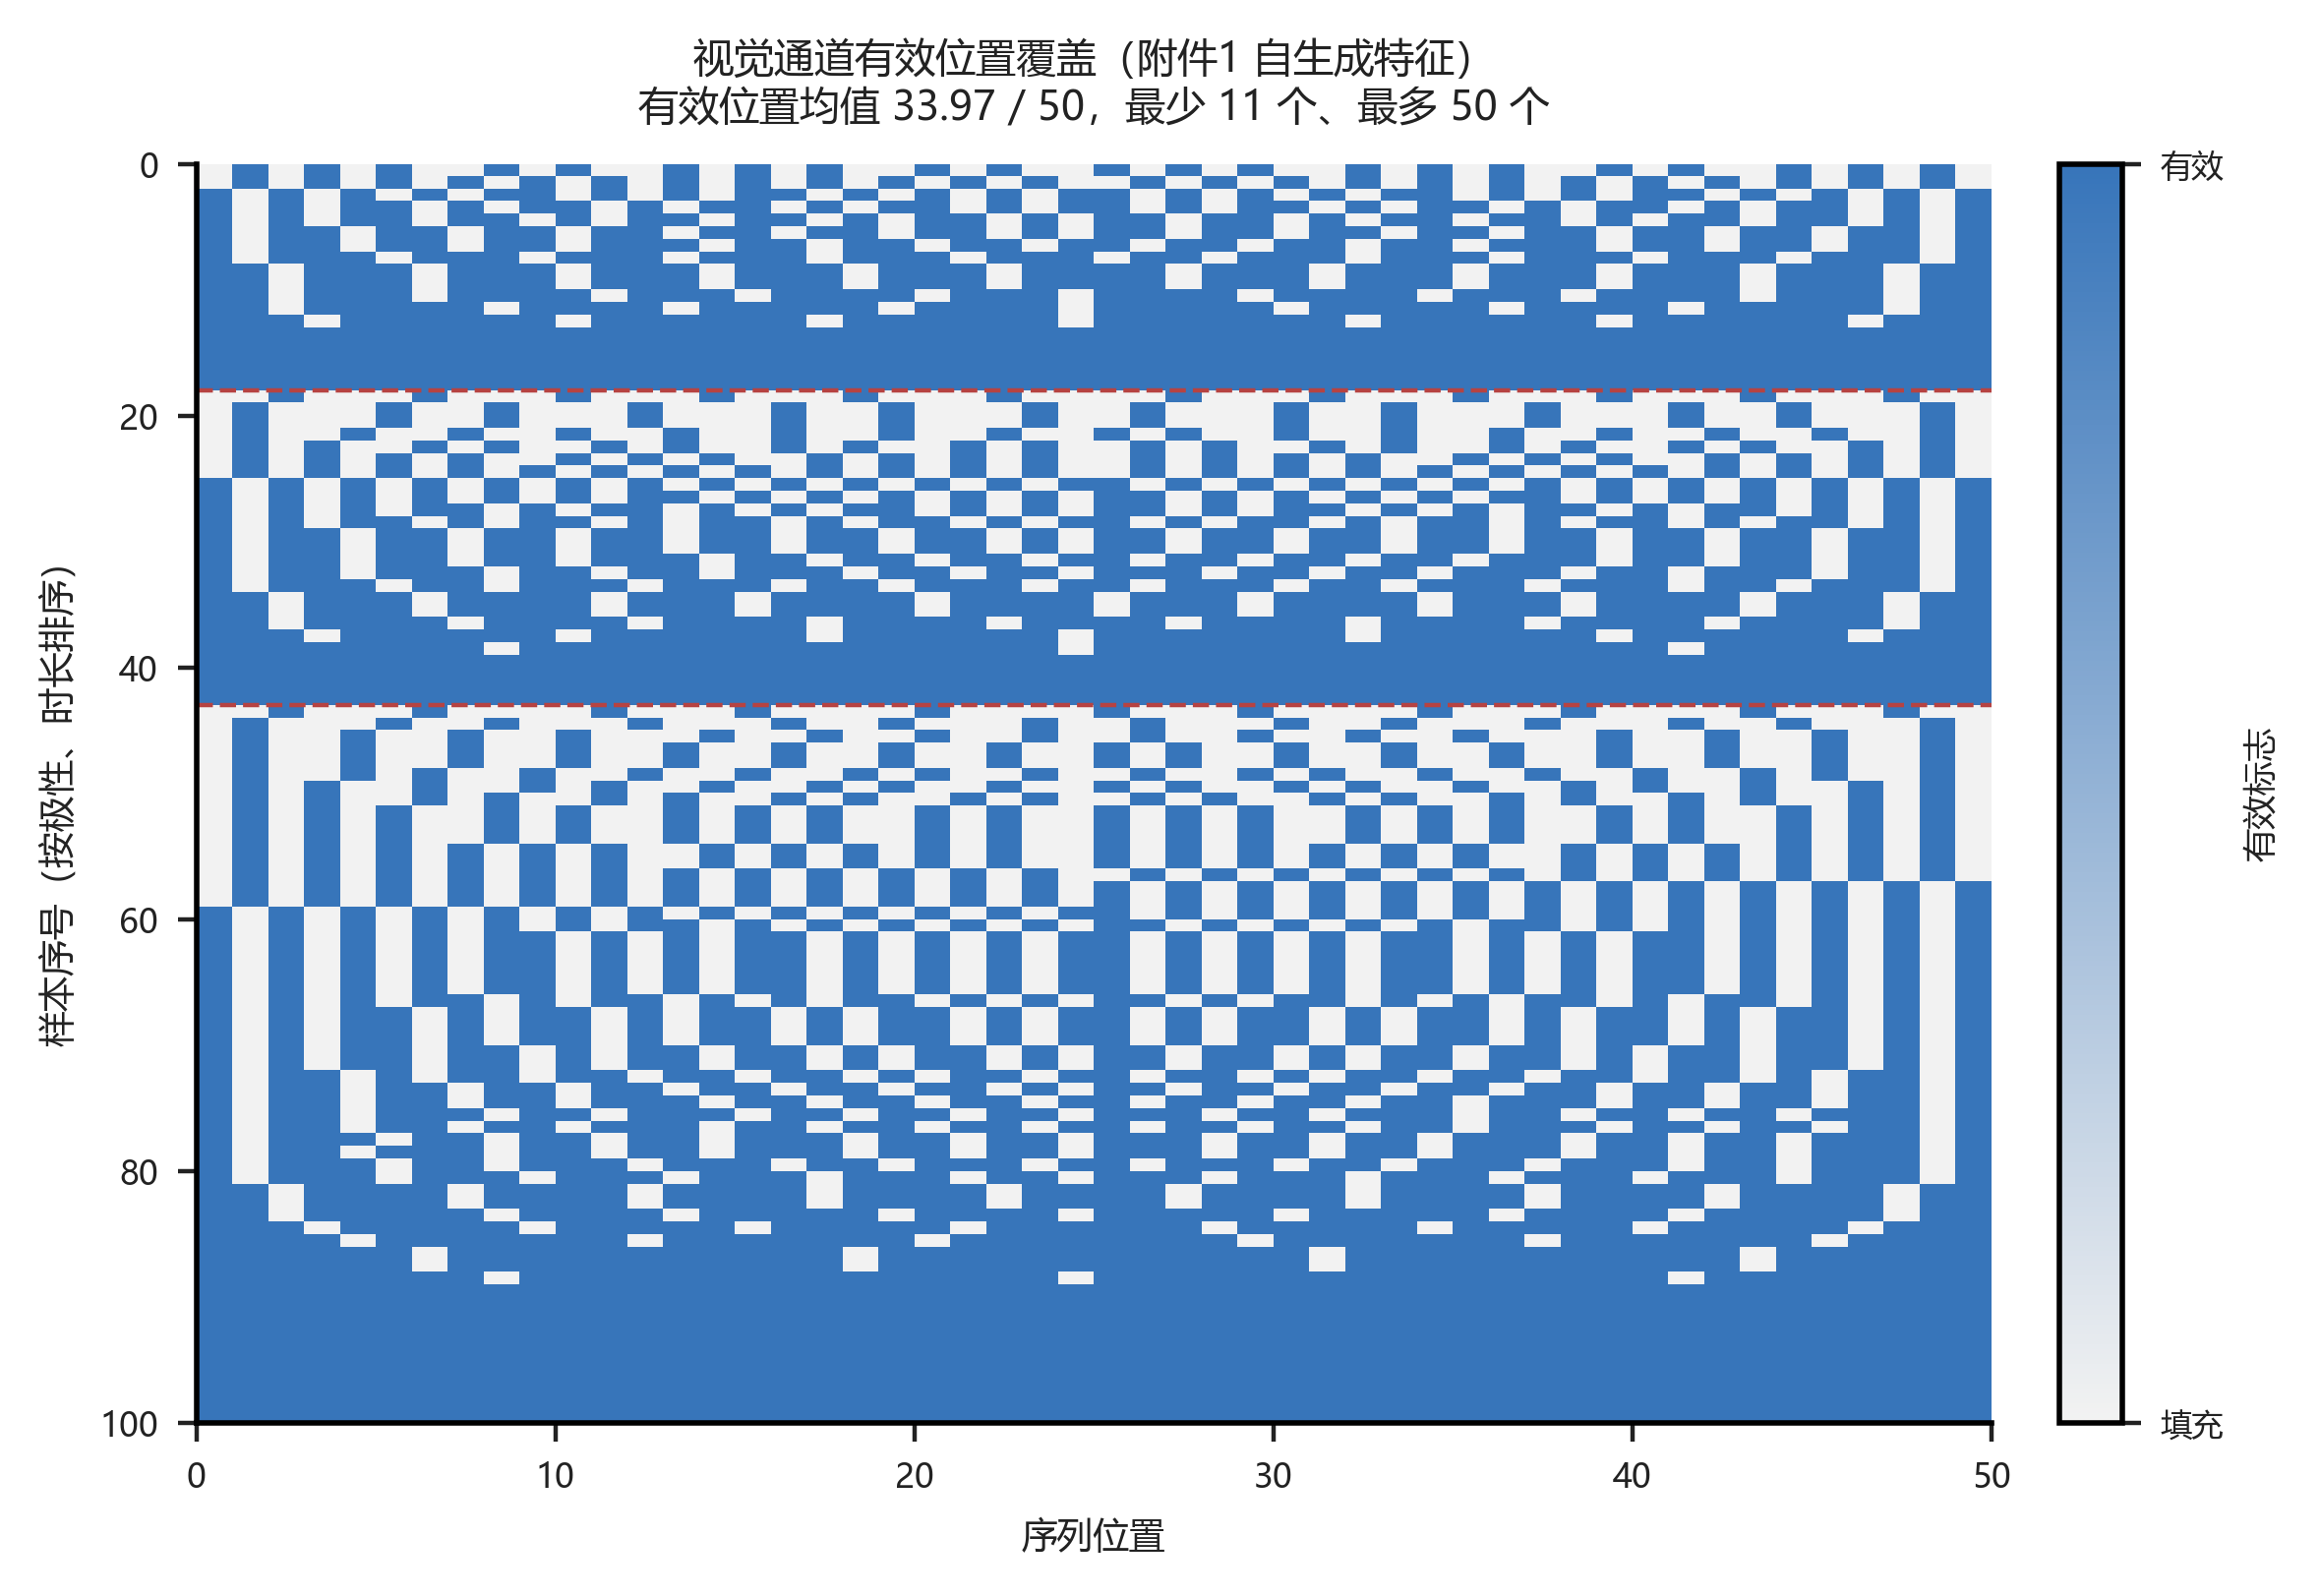
\includegraphics[width=0.86\textwidth]{Q1/figures/fig_q1_04_vision_coverage.png}
\caption{视觉通道有效位置覆盖与有效长度分布}
\label{fig:q1cov}
\end{figure}

覆盖图显示视觉通道的填充位置集中在每个样本序列的后段，且片段越短填充越多，原因是 5 帧/秒的抽帧在
短片段上不足以覆盖 50 个等分区间。该现象说明“局部时段视觉信息不可用”在真实数据中天然存在，而不是
人为构造，也为问题二的缺失建模提供了现实依据。三个极性区间的覆盖形态没有系统性差异，说明有效长度与
情感极性之间不存在明显关联。

\textbf{典型样本核验}的构造如下：选取一条时长 8.097 秒、含 30 个英文词元的样本，把文本词元落位、语音帧级能量与
视觉帧间灰度差画在同一条时间轴上，结果如图~\ref{fig:q1align} 所示。

\begin{figure}[htp!]
\centering
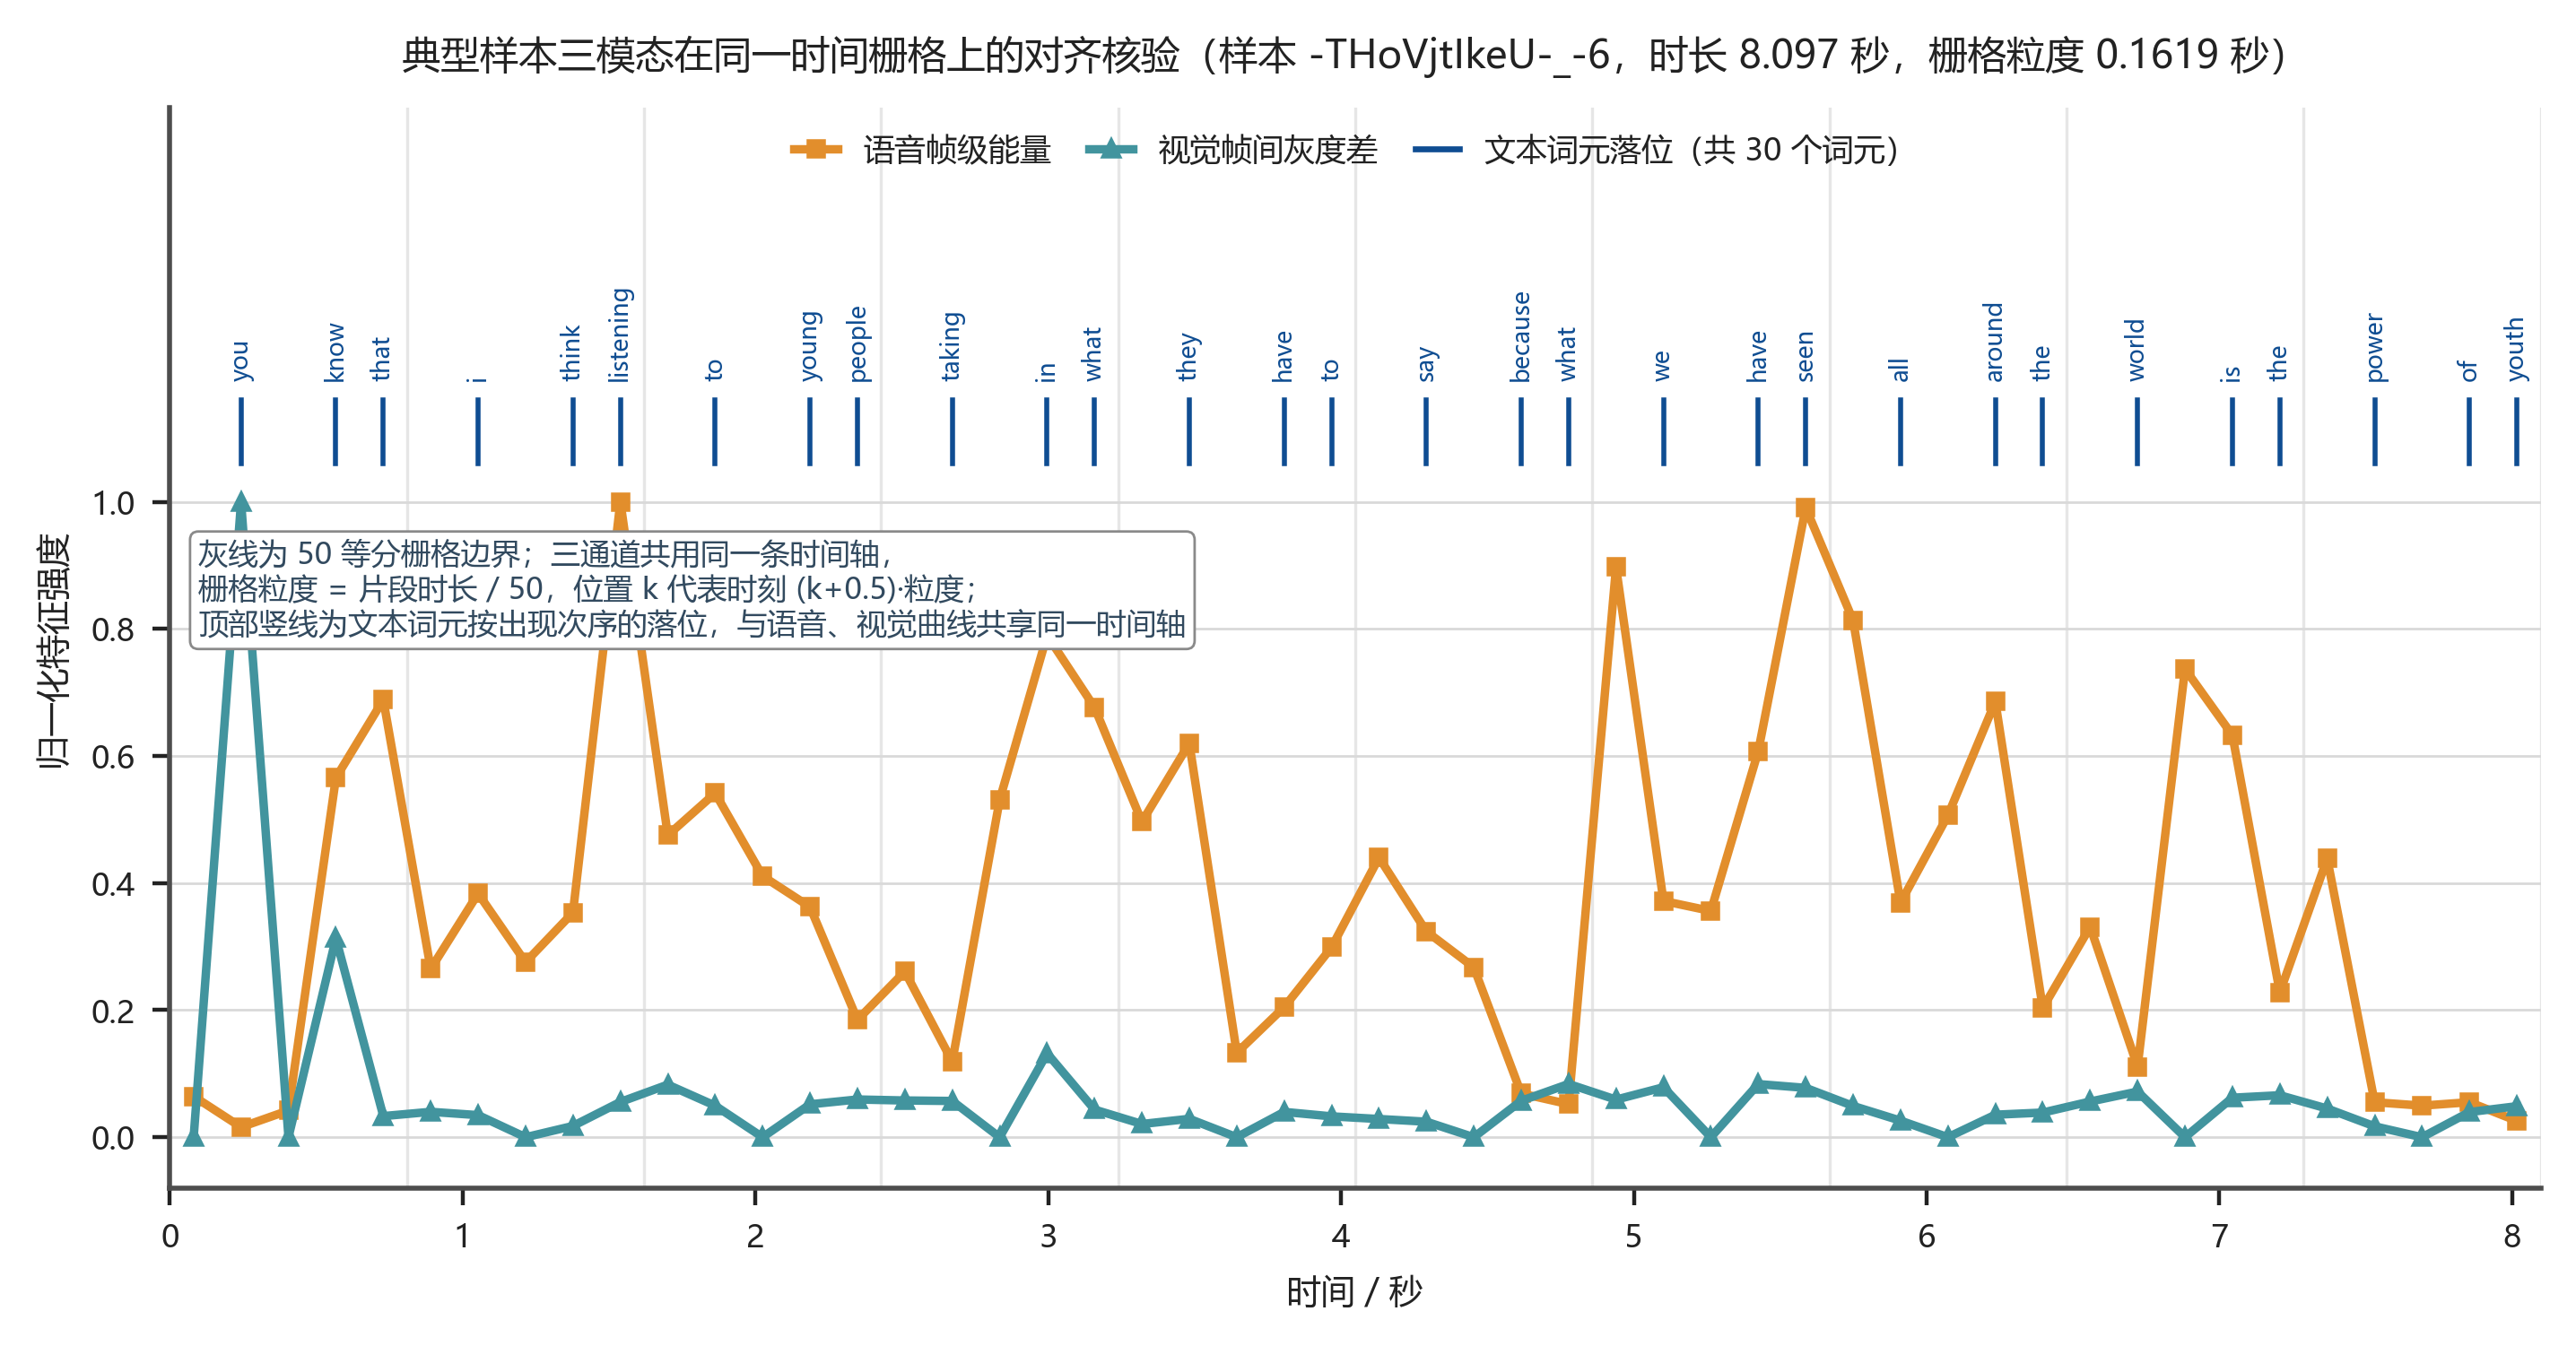
\includegraphics[width=0.99\textwidth]{Q1/figures/fig_q1_01_alignment.png}
\caption{典型样本三模态在同一时间栅格上的对齐核验}
\label{fig:q1align}
\end{figure}

图中灰色竖线为 50 等分栅格边界，顶部竖线为文本词元按出现次序的落位并标注了词元内容，橙色曲线为语音
帧级能量、青色曲线为视觉帧间灰度差。三类证据共享同一条时间轴：语音能量在第 4.7 秒与第 5.7 秒附近出现
两个明显峰值，视觉帧间灰度差在第 0.3 秒出现最大值随后衰减，文本词元则覆盖从第 0 秒到第 8 秒的全过程。
语音与视觉的起伏集中在片段前段，文本证据贯穿全程，这与后续问题三在解释层面得到的时段分布结论一致，
说明对齐规则确实把三模态放到了同一时间尺度，而不是把三路信号简单并置。

\subsection{可复现性说明}

特征提取所用的工具与版本为 ffmpeg 7.x、librosa 1.0.0、OpenCV 5.0.0、soundfile 0.14.0、NumPy 2.2.4。
关键参数为采样率 16 kHz、帧长 400、帧移 160、梅尔带数 64、抽帧率 5 帧/秒、帧尺寸 $112\times112$、
序列位置数 50、哈希维度 768、哈希盐值 mosei2026。全部参数与工具版本写入配置文件，随机种子固定为
20260924，重复运行应得到完全相同的特征文件。运行方式为在项目根目录执行特征提取脚本
\texttt{extract\_features.py}，输入为附件1 的原始视频与标注表，输出为特征文件、全量汇总表、
配置记录与核对结果四类产物。自生成特征与附件2 的对照口径逐项一致：文本 768 维、语音 74 维、视觉 35 维、
序列位置 50，因此可以直接接入问题二与问题三的模型接口。

\section{问题二模型建立与求解}

\subsection{问题分析与缺失结构刻画}

附件3 的 30 条样本提供了缺失的实测形态，如图~\ref{fig:q2miss} 所示。

\begin{figure}[htp!]
\centering
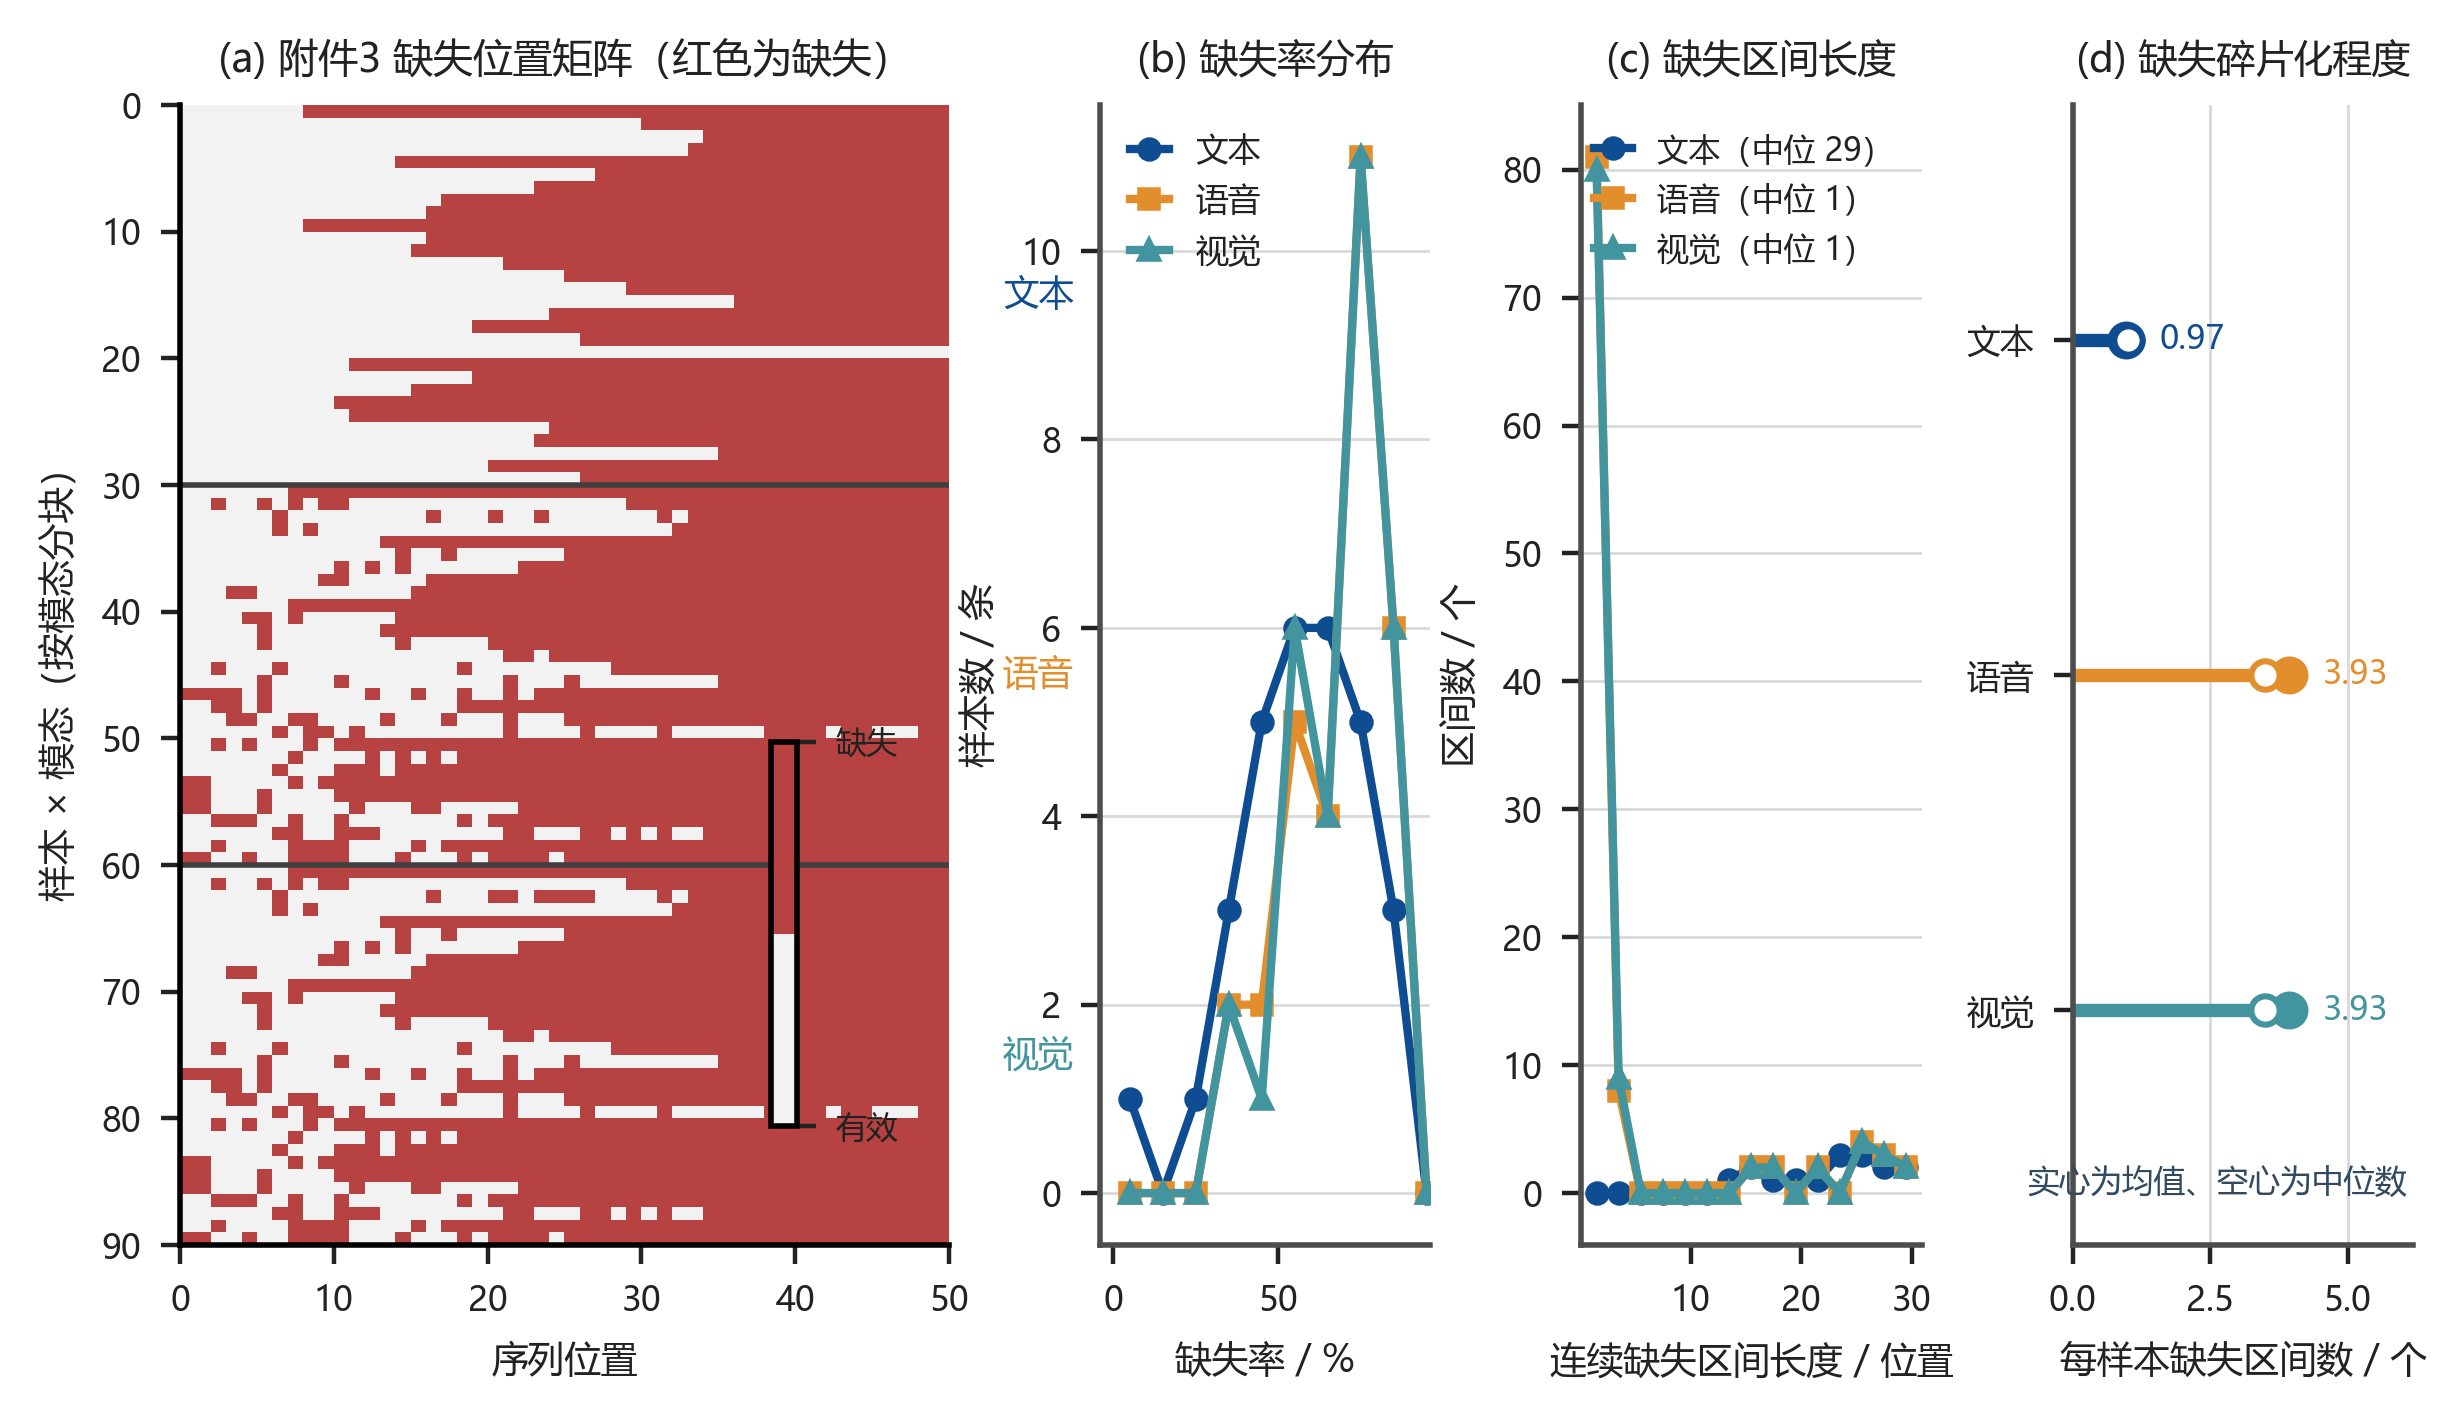
\includegraphics[width=0.99\textwidth]{Q2/figures/fig_q2_01_missing_pattern.png}
\caption{附件3 缺失位置矩阵、缺失率分布、区间长度与碎片化程度}
\label{fig:q2miss}
\end{figure}

缺失位置矩阵按模态分块显示，红色为缺失、灰色为有效。可以读出三个事实：语音与视觉的缺失区间几乎逐
样本一致，说明赛题在样本级别施加了同一条掩码，两个模态可能同时失效；缺失率分布上语音与视觉集中在
50\% 至 70\% 区间，文本分布更分散；连续缺失区间的长度上文本的中位长度为 29 个位置、语音与视觉的中位
长度为 1 个位置，说明文本的缺失以整段长区间为主、语音与视觉的缺失以碎小片段为主。碎片化程度上语音与
视觉每样本平均约 3.93 个缺失区间，文本约 0.97 个。这三条事实直接决定了模型设计：门控必须按位置独立
作用以应对碎片化缺失，掩码必须作为硬约束以应对长区间缺失，融合的归一化必须只统计可用位置。

三个候选方法在缺失场景下的适用性比较如下。插值或重建类方法先用可用模态补全缺失模态再融合，其优势是
可以复用完整模态的成熟结构，但在缺失率超过 50\% 时补全误差会主导最终预测，且补全结果不可复核；
固定权重融合按模态重要性加权求和，实现最简单，但在某一模态大面积缺失时会把噪声按固定权重带入；
缺失感知门控融合按位置、按模态动态分配可信度，代价是需要额外的门控参数并依赖缺失增强训练。本文选择
第三条路线，理由是它与本题“局部时段不可用”的缺失形态匹配，且门控权重本身可以复用为问题三的解释量。

\subsection{鲁棒融合模型}

\textbf{单模态时序编码}的构造如下：每个模态先做线性投影与层归一化，再经双向门控循环单元得到时序表示：

\begin{equation}
\mathbf{u}^{m}_{i,k}=\mathrm{GELU}\big(\mathrm{LN}(W^{m}_p\mathbf{x}^{m}_{i,k})\big),\qquad
\mathbf{h}^{m}_{i}=\mathrm{BiGRU}^{m}\big(\mathbf{u}^{m}_{i}\big),
\label{eq:encoder}
\end{equation}

其中 $\mathbf{h}^{m}_{i}\in\mathbb{R}^{L\times d}$，共享维度 $d=192$。层归一化的作用是稳定不同模态
在量纲上的差异，双向循环结构的作用是让每个位置同时看到前后文。

\textbf{可信度门控}的构造如下：门控权重由编码内容、可用性掩码与模态身份共同决定：

\begin{equation}
g^{m}_{i,k}=\sigma\Big(f_{\theta}\big([\mathbf{h}^{m}_{i,k};\ s^{m}_{i,k};\ \mathbf{e}_m]\big)\Big),
\qquad
\tilde{g}^{m}_{i,k}=g^{m}_{i,k}\,s^{m}_{i,k},
\label{eq:gate}
\end{equation}

$\mathbf{e}_m$ 为模态嵌入。掩码相乘是硬约束：缺失位置的门控权重恒为 0，缺失信息不进入融合。门控的
含义是“这个位置这个模态在当前样本中有多可信”，它既读取掩码，也读取编码内容，因此能够在掩码之外
识别出“虽然存在但内容异常”的位置。

\textbf{掩码归一化融合与跨模态注意力}的构造如下：以可用门控权重为分母做加权平均，再对融合序列做自注意力：

\begin{equation}
\mathbf{z}^{\mathrm{fuse}}_{i,k}
=\frac{\sum_m \tilde{g}^{m}_{i,k}\,W^{m}_f\mathbf{h}^{m}_{i,k}}
{\max\big(\sum_m \tilde{g}^{m}_{i,k},\ \epsilon\big)},
\qquad
\mathbf{Z}_i=\mathrm{LN}\Big(\mathbf{z}^{\mathrm{fuse}}_i+\mathrm{MHA}(\mathbf{z}^{\mathrm{fuse}}_i)\Big),
\label{eq:fusion}
\end{equation}

自注意力以“全部门控权重为零”作为键掩码，保证填充位置不参与注意力计算。分母只统计可用权重，因此
缺失多少模态都不会把表示缩放到 0 附近，这是该结构与简单平均融合的关键区别。

\textbf{跨模态交互支路}的构造如下：时序门控融合之外另加一条全局支路：把各模态的时序均值、时序最大值与可用
比例拼成跨模态描述向量，经两层感知机得到全局摘要，再与位置聚合结果相加。该支路的作用是表达“哪些模态
一致、哪些模态被削弱”这类整体结构，在时序局部信息因缺失而减少时提供互补证据。

\textbf{位置聚合与目标函数}的构造如下：位置权重由可学习查询打分后按可用位置归一化：

\begin{equation}
\beta_{i,k}=\frac{s_{i,k}\exp\!\big(q^\top \phi(\mathbf{Z}_{i,k})\big)}
{\sum_{k'} s_{i,k'}\exp\!\big(q^\top \phi(\mathbf{Z}_{i,k'})\big)},
\qquad
\mathbf{z}_i=\sum_k \beta_{i,k}\mathbf{Z}_{i,k},
\label{eq:pool}
\end{equation}

\begin{equation}
\mathcal{L}=\underbrace{-\sum_{c=1}^{3} w_c\, y^{\mathrm{cls}}_{i,c}\log \hat{p}_{i,c}}_{\text{类别加权交叉熵}}
+\lambda\underbrace{\mathrm{Huber}\big(y^{\mathrm{reg}}_i-\hat{y}^{\mathrm{reg}}_i\big)}_{\text{强度回归}},
\qquad
w_c=\frac{N}{3N_c},\quad \lambda=1,
\label{eq:loss}
\end{equation}

$N_c$ 为第 $c$ 类的样本数。类别权重的作用是缓解中性类样本偏少带来的梯度偏置；Huber 损失在残差较大时
退化为线性，作用是抑制少数极端标注对回归的影响。模型结构原理如图~\ref{fig:q2principle} 所示。

\begin{figure}[htp!]
\centering
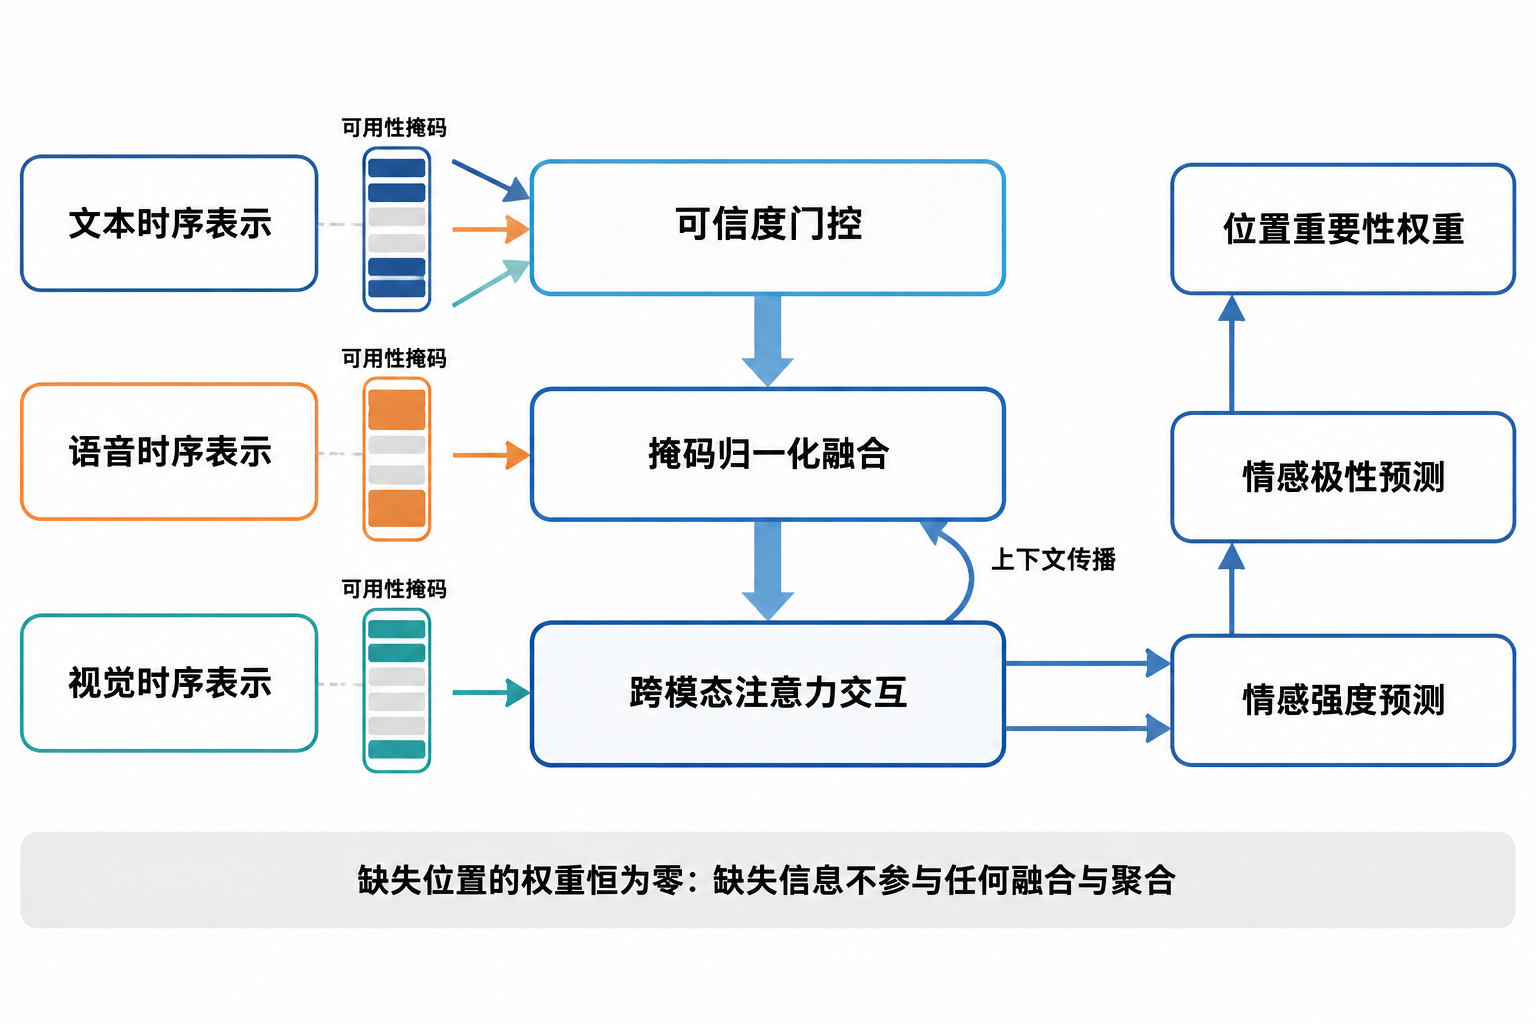
\includegraphics[width=0.90\textwidth]{手绘图/鲁棒融合原理图.png}
\caption{缺失感知鲁棒融合机制原理图}
\label{fig:q2principle}
\end{figure}

该图把模型拆成输入端、机制区与输出端三段。输入端为三个模态的时序表示与各自的可用性掩码；机制区自上
而下为可信度门控、掩码归一化融合与跨模态注意力交互三层，右侧的弧线表示上下文传播；输出端为位置重要性
权重与两个预测头。底部约束条写明“缺失位置的权重恒为零：缺失信息不参与任何融合与聚合”，对应
式~\eqref{eq:gate} 的硬约束。图的提示词保存在手绘图/鲁棒融合原理图提示词.md。

\textbf{约束条件}的构造如下：一是缺失约束：$s^{m}_{i,k}=0$ 时必有 $\tilde{g}^{m}_{i,k}=0$；二是归一化约束：
$\sum_m\tilde{g}^{m}_{i,k}\in\{0,1,2,3\}$ 且分母不为零；三是阈值约束：三分类决策阈值只在验证集上选择；
四是数据约束：训练、验证与专项测试使用同一特征版本与同一输入接口。

\subsection{训练方案与消融实验}

\textbf{训练流程}的构造如下：训练分两阶段。第一阶段为单模态编码器预训练：每个模态单独接三分类头与回归头训练，
文本 24 轮、语音 24 轮、视觉 24 轮，批大小 64、学习率 $2\times10^{-3}$、权重衰减 $10^{-4}$；
训练完成后冻结编码器并缓存编码序列。第二阶段为融合模型训练：在缓存的编码序列上训练融合结构，
批大小 128、学习率 $1.5\times10^{-3}$、余弦退火至初始值的 0.1、共 30 轮、梯度裁剪阈值 5.0。
两阶段方案的动机是把代价最高的序列编码与代价较低的融合训练解耦，使缺失增强策略可以在同一份缓存上
快速比较。验证集上的基础性能如表~\ref{tab:encoder} 所示。

\begin{table}[htp!]
\centering
\caption{单模态编码器在验证集上的基础性能}
\label{tab:encoder}
\renewcommand\arraystretch{1.25}
\begin{tabular}{|c|c|c|c|c|}
\hline
模态 & 准确率 & 宏平均 F1 & 强度平均绝对误差 & 强度皮尔逊相关系数 \\
\hline
文本 & 0.5907 & 0.5721 & 0.6349 & 0.5979 \\
\hline
语音 & 0.3901 & 0.3620 & 0.9222 & 0.0667 \\
\hline
视觉 & 0.4135 & 0.3971 & 0.8323 & 0.2126 \\
\hline
\end{tabular}
\end{table}

表中数据说明文本通道单独就能达到 0.5907 的准确率与 0.6349 的强度误差，而语音与视觉的准确率接近随机
水平、强度相关系数分别为 0.0667 与 0.2126。这一结果限定了后续融合的性能上限：融合只能在文本之外
补充有限的语音与视觉信息，因此融合模型的准确率不会显著高于仅文本，其价值应体现在缺失条件下的稳定性。

\textbf{缺失增强策略比较}的构造如下：四种策略在同一份缓存上训练同一结构，结果如表~\ref{tab:strategy} 所示。

\begin{table}[htp!]
\centering
\caption{四种缺失增强策略在主模型上的验证集性能}
\label{tab:strategy}
\renewcommand\arraystretch{1.2}
\small
\setlength{\tabcolsep}{4pt}
\begin{tabular}{|p{3.6cm}|c|c|c|c|}
\hline
策略 & 准确率 & 宏平均 F1 & 强度平均绝对误差 & 强度皮尔逊相关系数 \\
\hline
无缺失增强 & 0.5646 & 0.5376 & 0.6429 & 0.5823 \\
\hline
轻度增强（缺失率 0.05--0.30） & 0.5728 & 0.5400 & 0.6476 & 0.5844 \\
\hline
重度增强（缺失率 0.10--0.60） & 0.5728 & 0.5442 & 0.6465 & 0.5826 \\
\hline
课程式增强（缺失率 0.05 升至 0.55，最终采用） & 0.5632 & 0.5271 & 0.6418 & 0.5852 \\
\hline
\end{tabular}
\end{table}

四种策略的差异很小：准确率极差 0.0096、强度误差极差 0.0058。这一结果本身是一个结论：在本文特征下，
缺失增强对无缺失验证集的性能影响有限，其作用主要体现在缺失条件下的退化幅度，因此本文以验证集强度误差
为主选择准则，最终采用课程式增强，并在后续用缺失率扫描检验其鲁棒性。

\textbf{融合结构消融}的构造如下：逐项替换融合结构，结果如图~\ref{fig:q2abl} 所示。

\begin{figure}[htp!]
\centering
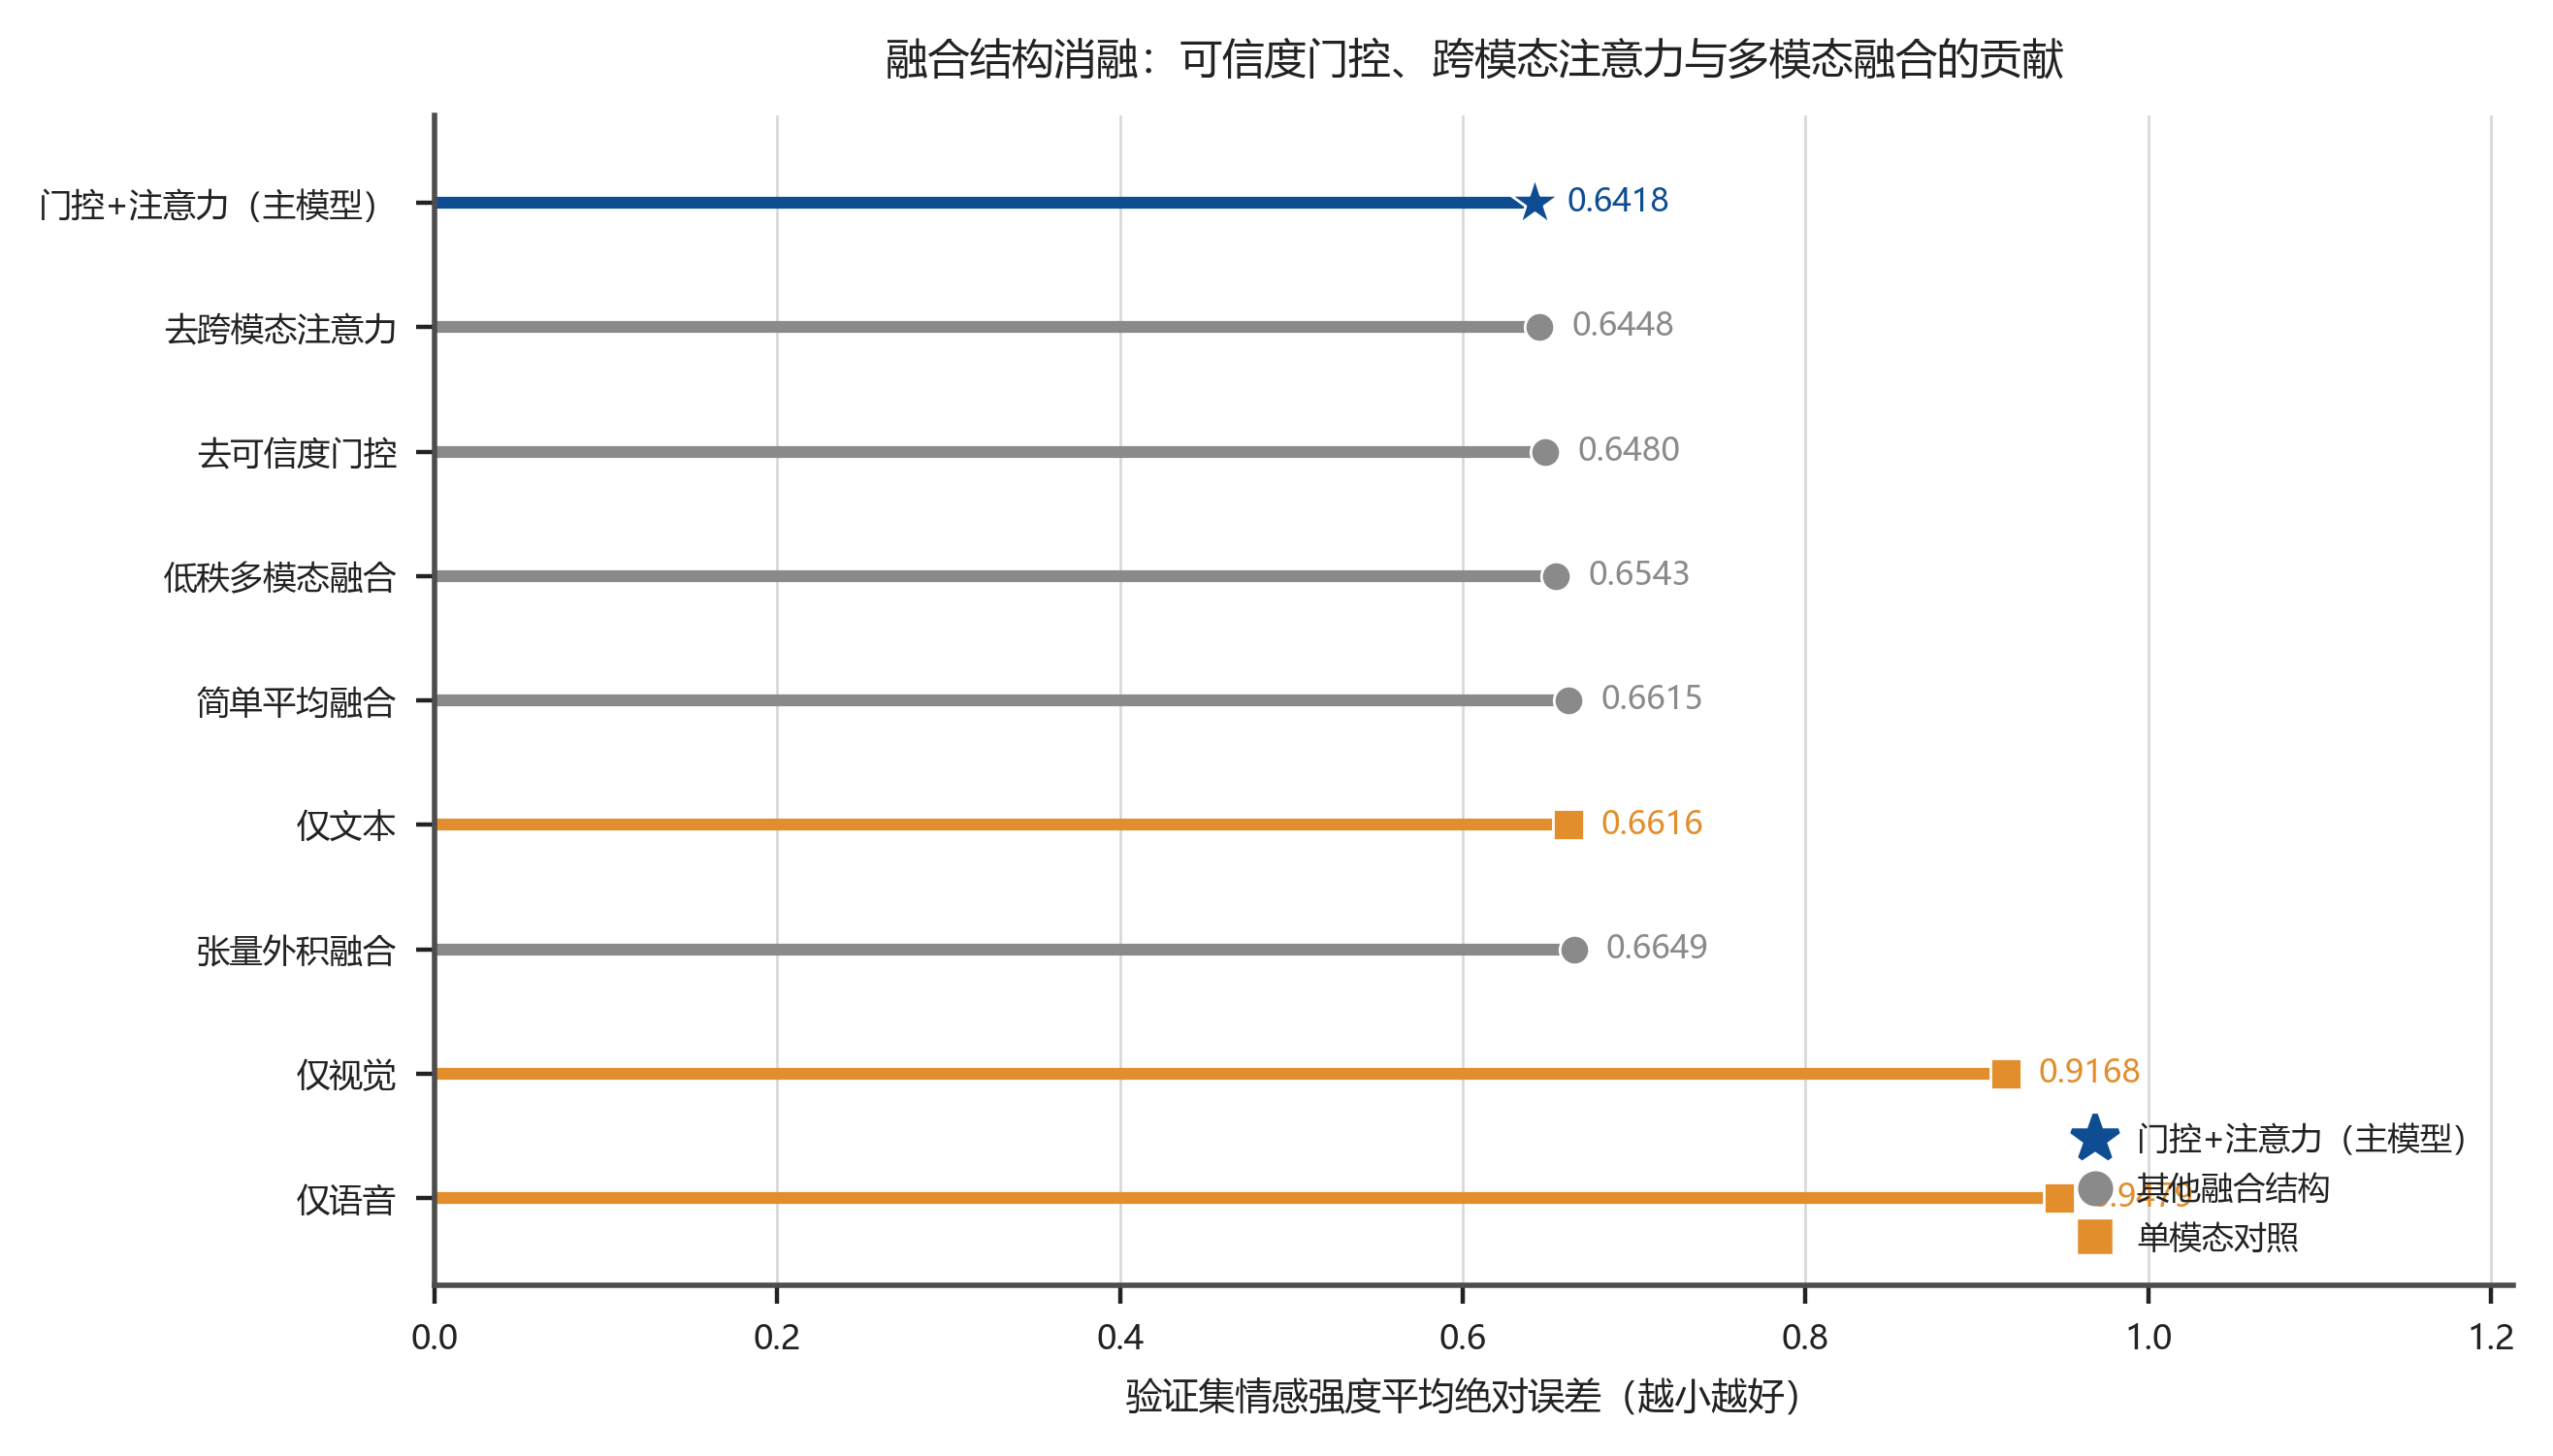
\includegraphics[width=0.92\textwidth]{Q2/figures/fig_q2_06_ablation.png}
\caption{融合结构消融：门控、注意力与多模态融合的贡献}
\label{fig:q2abl}
\end{figure}

按验证集强度平均绝对误差从小到大排列，主模型为 0.6418，去跨模态注意力为 0.6448，去可信度门控为
0.6480，低秩多模态融合为 0.6543，简单平均融合为 0.6615，仅文本为 0.6616，张量外积融合为 0.6649，
仅视觉为 0.9168，仅语音为 0.9479。三点解释：门控与注意力各自都有正贡献，去掉任意一个都会使误差上升；
张量外积融合参数最多但在本文的编码维度下过拟合，误差反而高于简单平均融合；仅语音与仅视觉的误差接近
0.9 以上，说明在本文特征下这两个模态单独不足以支撑强度回归。需要同时指出的是，主模型在无缺失的极性
准确率（0.5632）并不高于简单平均融合（0.5907）与仅文本（0.5810），而强度误差顺序恰好相反。因此本文
的结论是：融合结构主要改善强度回归的稳定性与缺失条件下的退化幅度，而不是无条件提高无缺失时的极性准确率。

\subsection{缺失类型、位置与时长的规律分析}

\textbf{缺失率规律}的构造如下：对全模态同时缺失与单模态缺失分别扫描缺失率 0.0 至 0.7，每个缺失率重复 3 次随机
缺失施加，结果如图~\ref{fig:q2rate} 所示。

\begin{figure}[htp!]
\centering
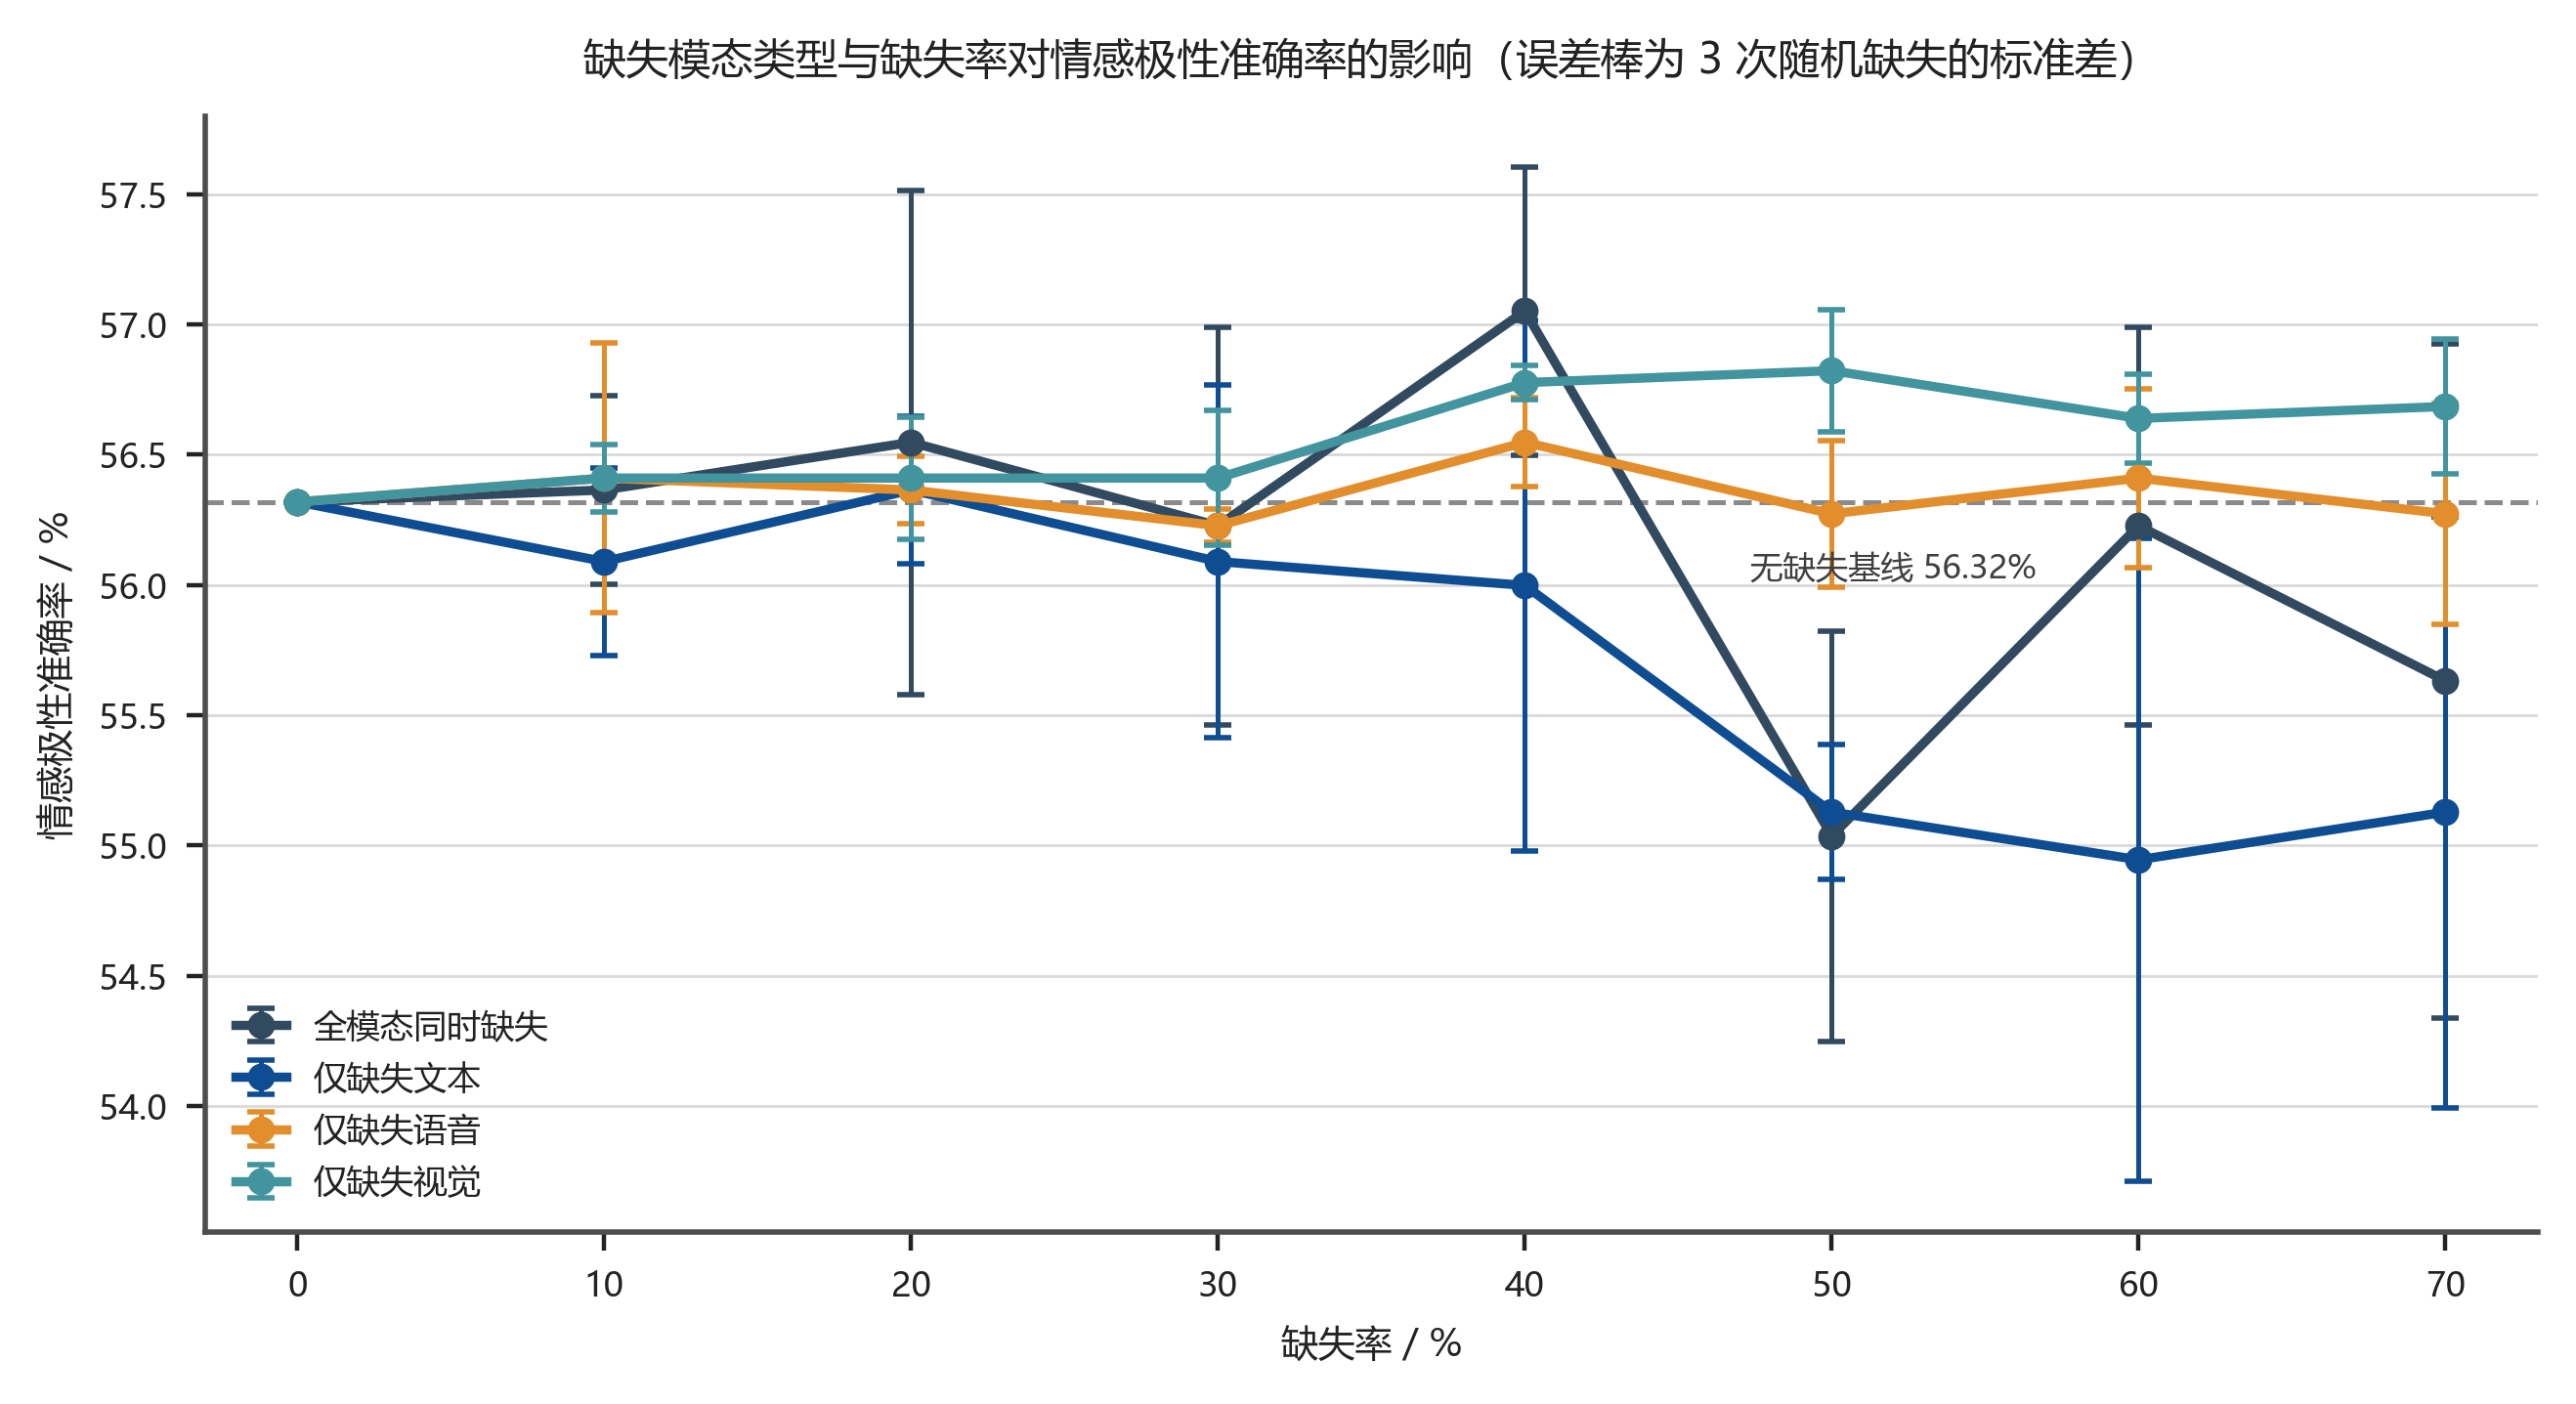
\includegraphics[width=0.92\textwidth]{Q2/figures/fig_q2_02_rate_curves.png}
\caption{缺失模态类型与缺失率对情感极性准确率的影响}
\label{fig:q2rate}
\end{figure}

全模态同时缺失时准确率从 0.5632 降到 0.5563，误差从 0.6418 升到 0.6674，退化幅度温和且有波动，
说明门控与掩码归一化确实起到了稳定作用。单模态缺失的差异更明显：仅缺失文本时误差从 0.6418 升到
0.6649，仅缺失语音时误差在 0.6394 至 0.6438 之间波动，仅缺失视觉时误差在 0.6417 至 0.6440 之间波动，
两个模态的误差曲线甚至在中段低于无缺失基线。这一对照给出明确结论：文本是本文特征下最关键的模态，
语音与视觉在缺失率 0.7 以内的贡献可以被其余模态替代，替代能力来自文本通道的高覆盖率与较强的单模态性能。

\textbf{缺失时长规律}的构造如下：在序列前段、中段、后段分别施加长度为 5 至 25 的连续缺失窗口，结果如
图~\ref{fig:q2dur} 所示。

\begin{figure}[htp!]
\centering
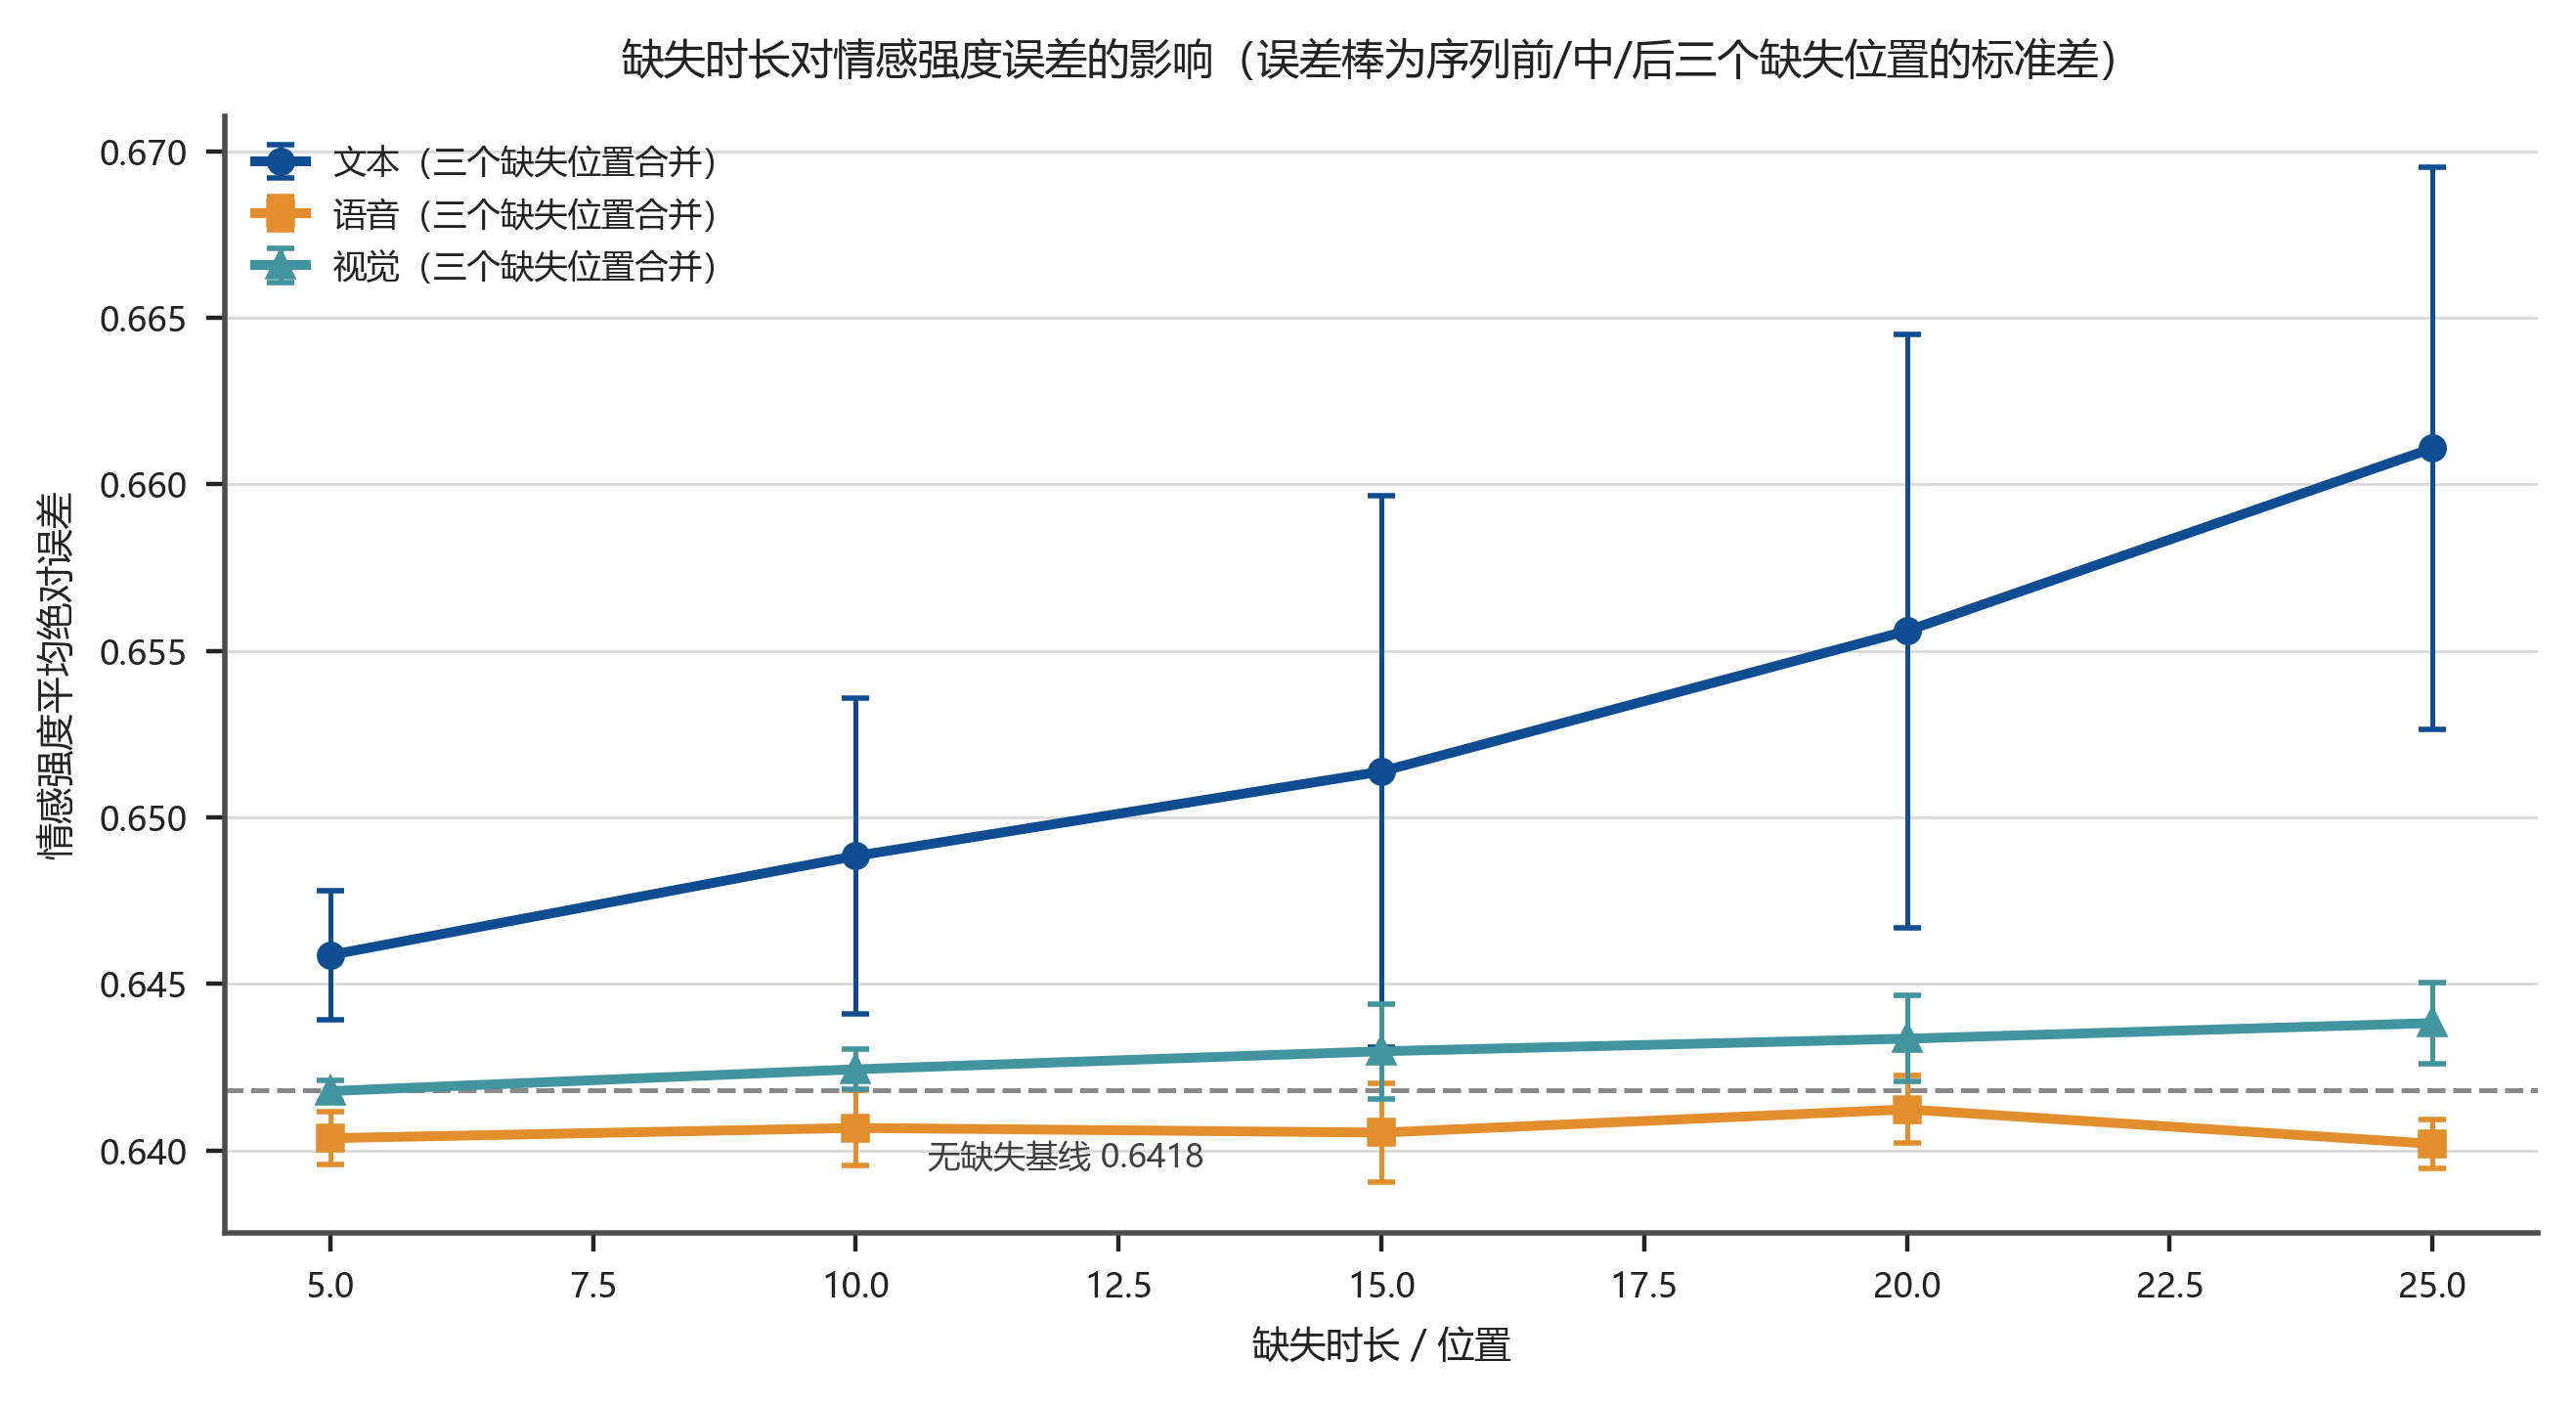
\includegraphics[width=0.92\textwidth]{Q2/figures/fig_q2_05_duration_error.png}
\caption{缺失时长对情感强度误差的影响}
\label{fig:q2dur}
\end{figure}

误差随缺失时长单调上升：文本从 5 个位置的 0.6459 升到 25 个位置的 0.6609，语音从 0.6405 升到
0.6413，视觉从 0.6416 升到 0.6440。文本的上升斜率最大，语音几乎平坦。长度为 25 的连续缺失下，文本
前段缺失的误差最高（0.6724），中段最低（0.6522），后段居中（0.6586）；语音与视觉在三个位置上的差异
均在 0.002 以内。这说明缺失“发生在哪里”对文本通道有实质影响，对语音与视觉影响很小。

\textbf{缺失位置与缺失时长的联合响应面}的构造如下：在位置×时长网格上计算强度误差，结果如
图~\ref{fig:q2surf} 所示。

\begin{figure}[htp!]
\centering
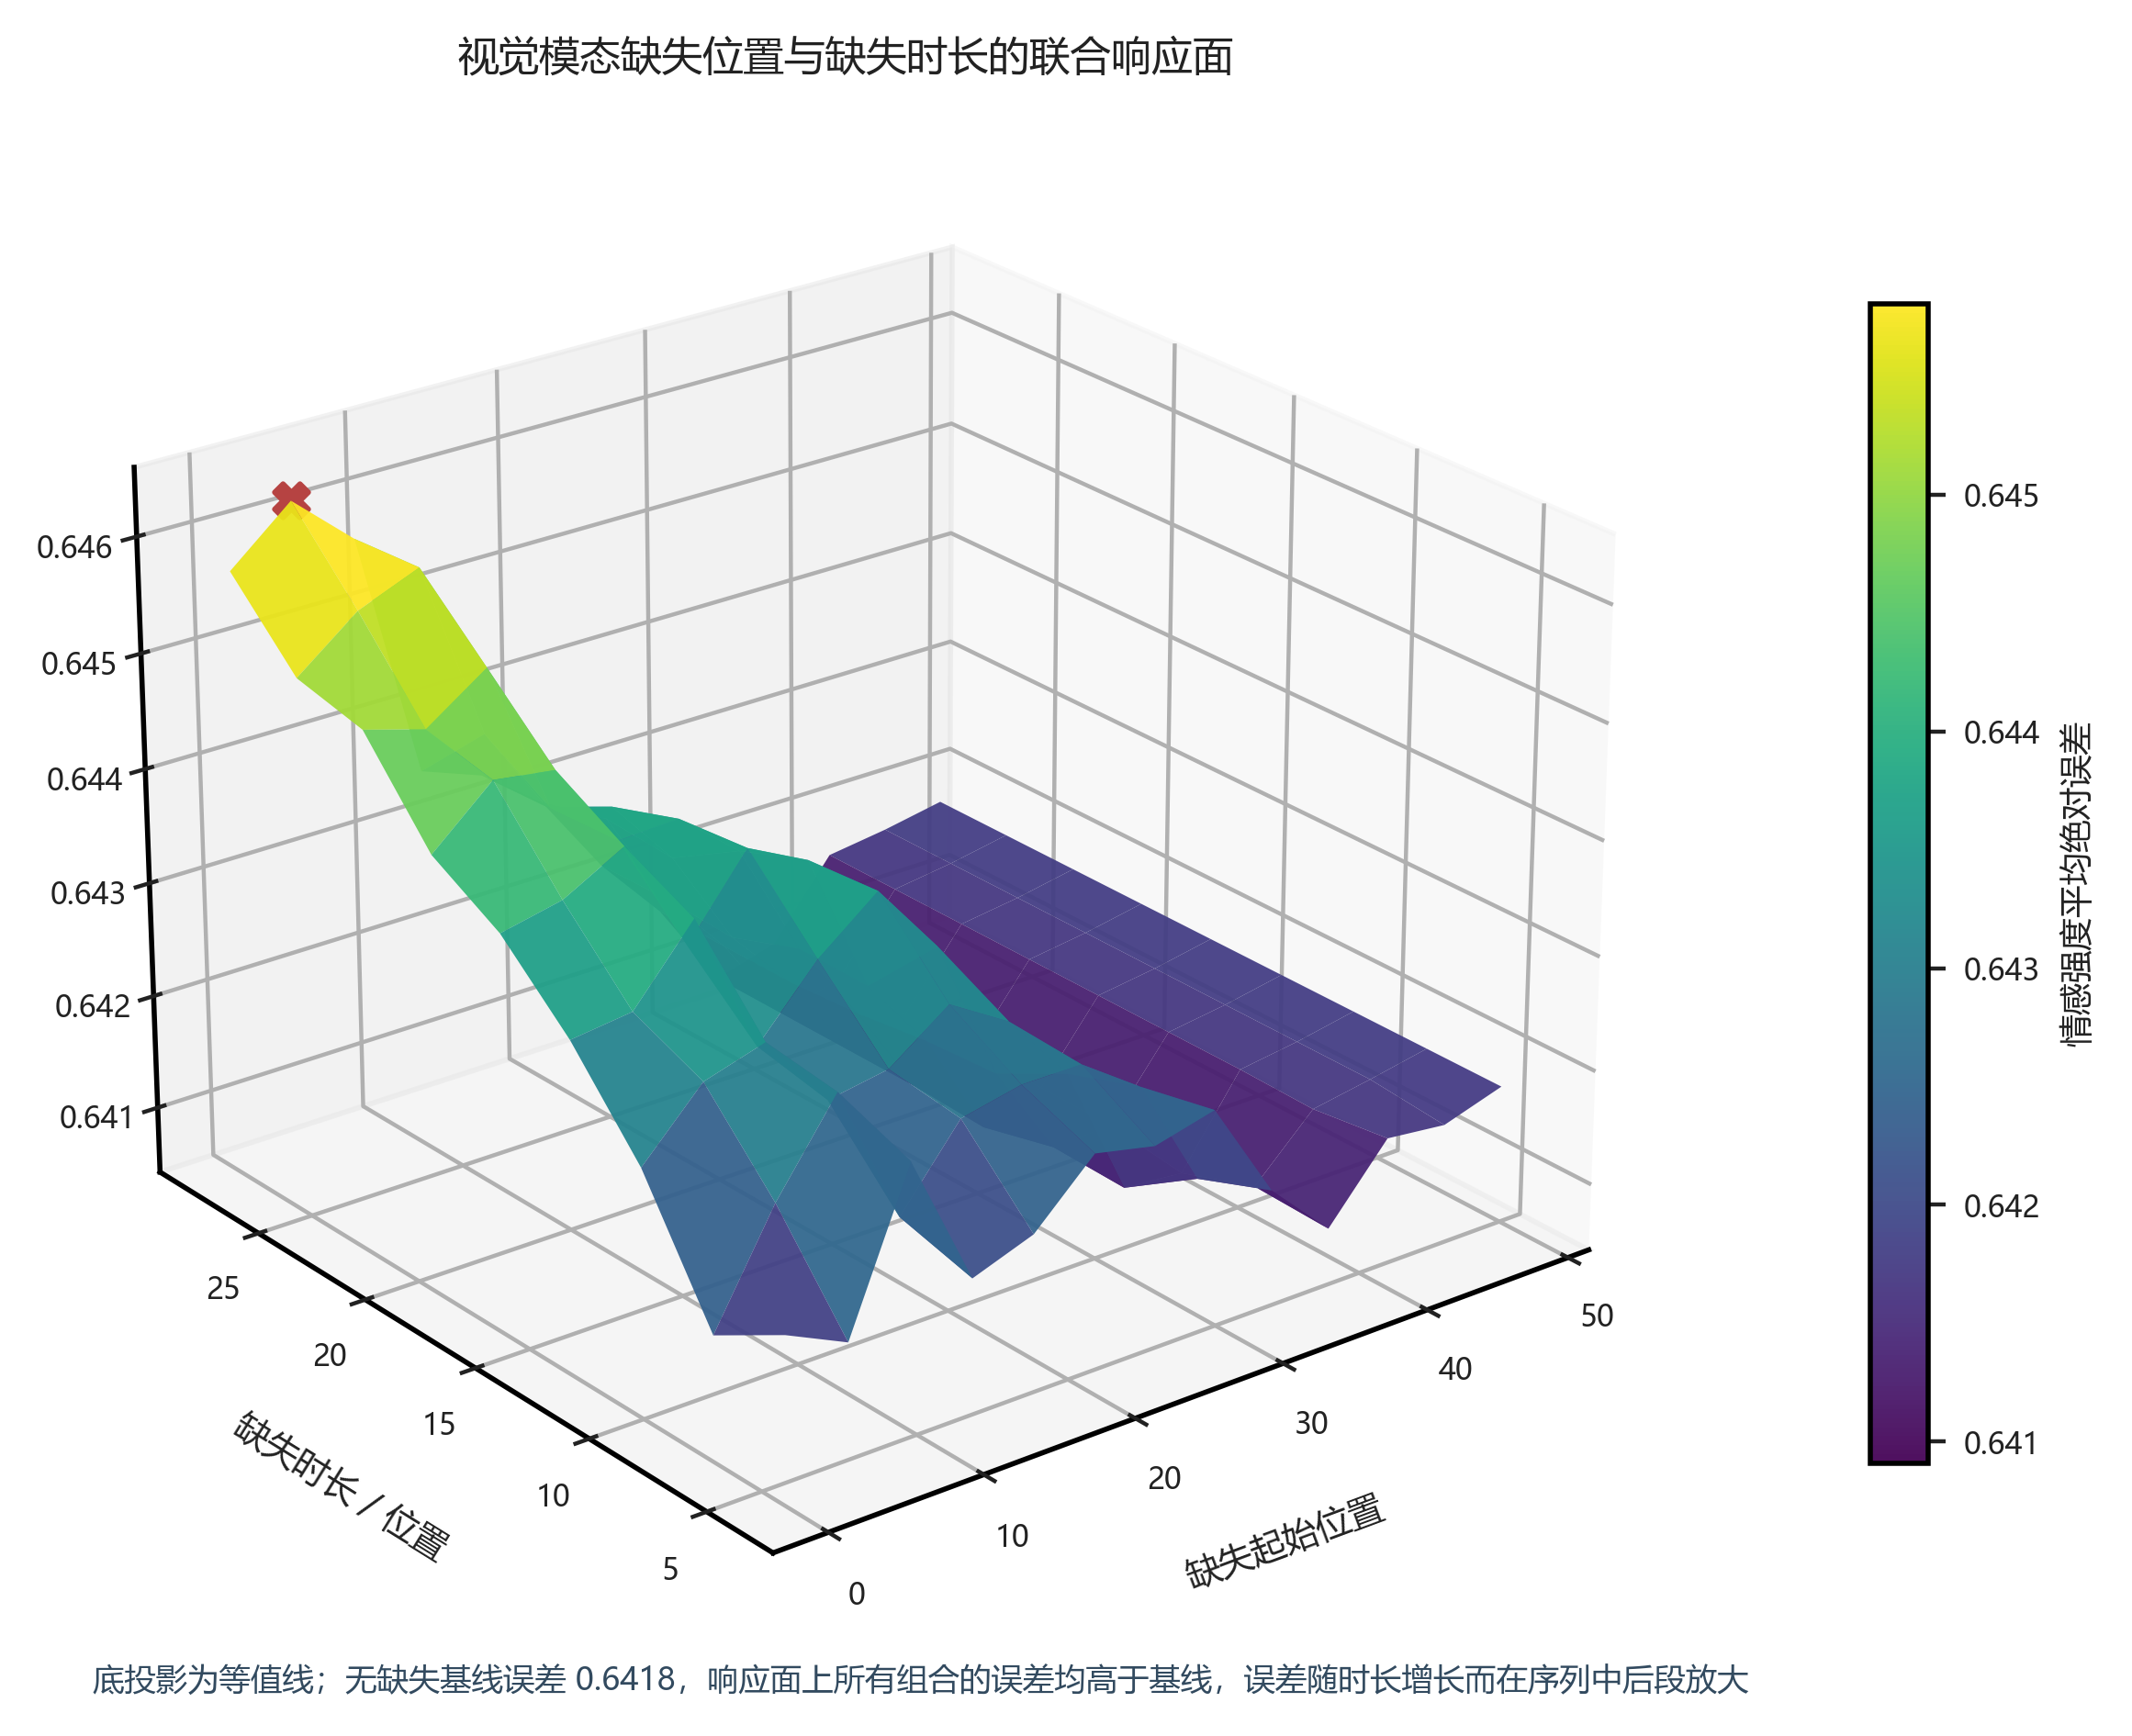
\includegraphics[width=0.80\textwidth]{Q2/figures/fig_q2_03_response_surface.png}
\caption{视觉模态缺失位置与缺失时长的联合误差响应面}
\label{fig:q2surf}
\end{figure}

响应面显示误差随时长单调增长，且在序列后段缺失时抬升更明显；无缺失基线误差为 0.6418，响应面上所有
组合的误差都高于该基线。曲面的形态说明缺失时长是主导因素，缺失位置是次要因素，两者的交互作用体现为
“长缺失落在后段”时误差最大。

\subsection{参数敏感度分析}

在验证集上固定模型参数，只扰动输入缺失参数，考察四个缺失相关参数与门控阈值的影响幅度，结果如
图~\ref{fig:sens1} 所示。

\begin{figure}[htp!]
\centering
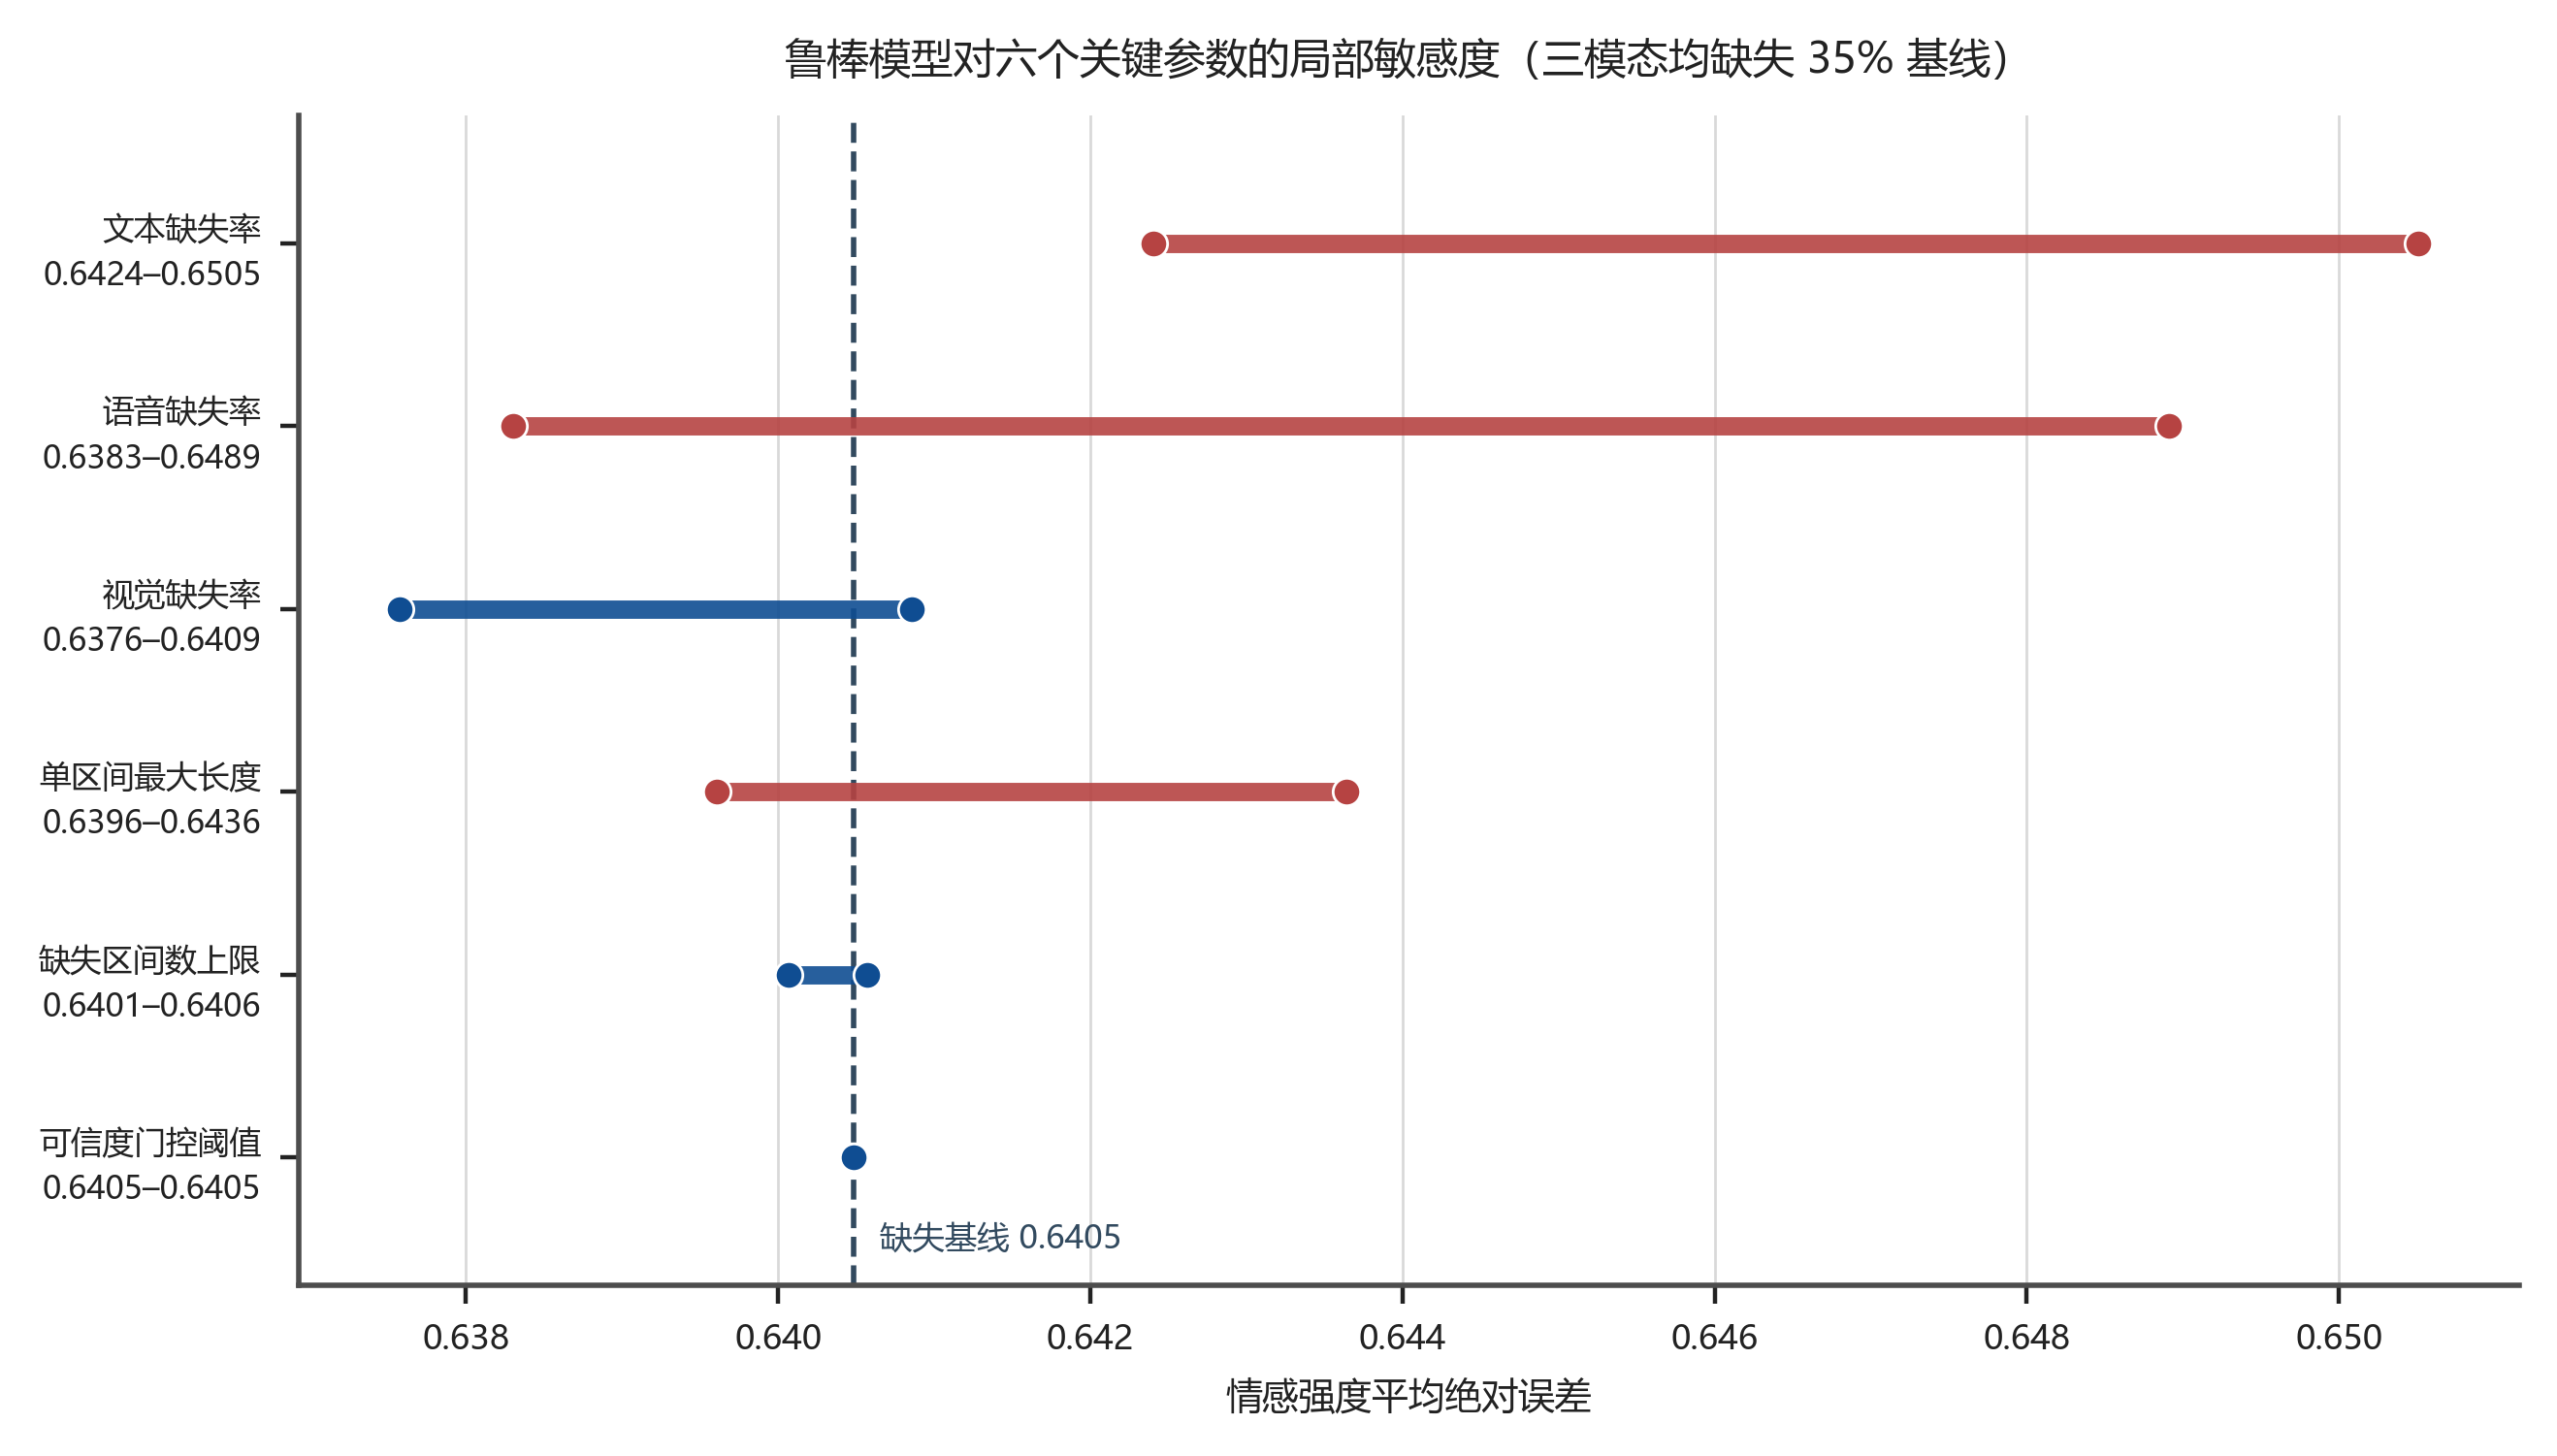
\includegraphics[width=0.90\textwidth]{灵敏度分析/figures/fig_sens_01_local_tornado.png}
\caption{鲁棒模型对六个关键参数的局部敏感度}
\label{fig:sens1}
\end{figure}

在三模态均缺失 35\% 的基线下，影响幅度最大的两个参数是语音缺失率（0.010609）与文本缺失率（0.008101），
单区间最大长度次之（0.004032）与视觉缺失率（0.003278），缺失区间数上限只有 0.000504，可信度门控阈值
的影响幅度为 0。三点解释：缺失“有多少”比缺失“怎么分布”更重要，因为三个缺失率参数的影响幅度都大于
区间长度与区间数；门控阈值不影响输出，说明模型的最大类概率在验证集上几乎全部高于 0.95，阈值在
0.05 至 0.95 内不产生惩罚差异；缺失区间数不敏感是因为在固定缺失率下把同样的缺失总量拆得更碎并不会
改变门控的逐位置判断。无缺失基线下除三个缺失率参数之外的所有参数影响幅度均为 0，说明这些参数只有在
已存在缺失时才起作用。

参数影响幅度、缺失率与缺失时长效应以及联合响应面汇总如图~\ref{fig:sens2} 所示。

\begin{figure}[htp!]
\centering
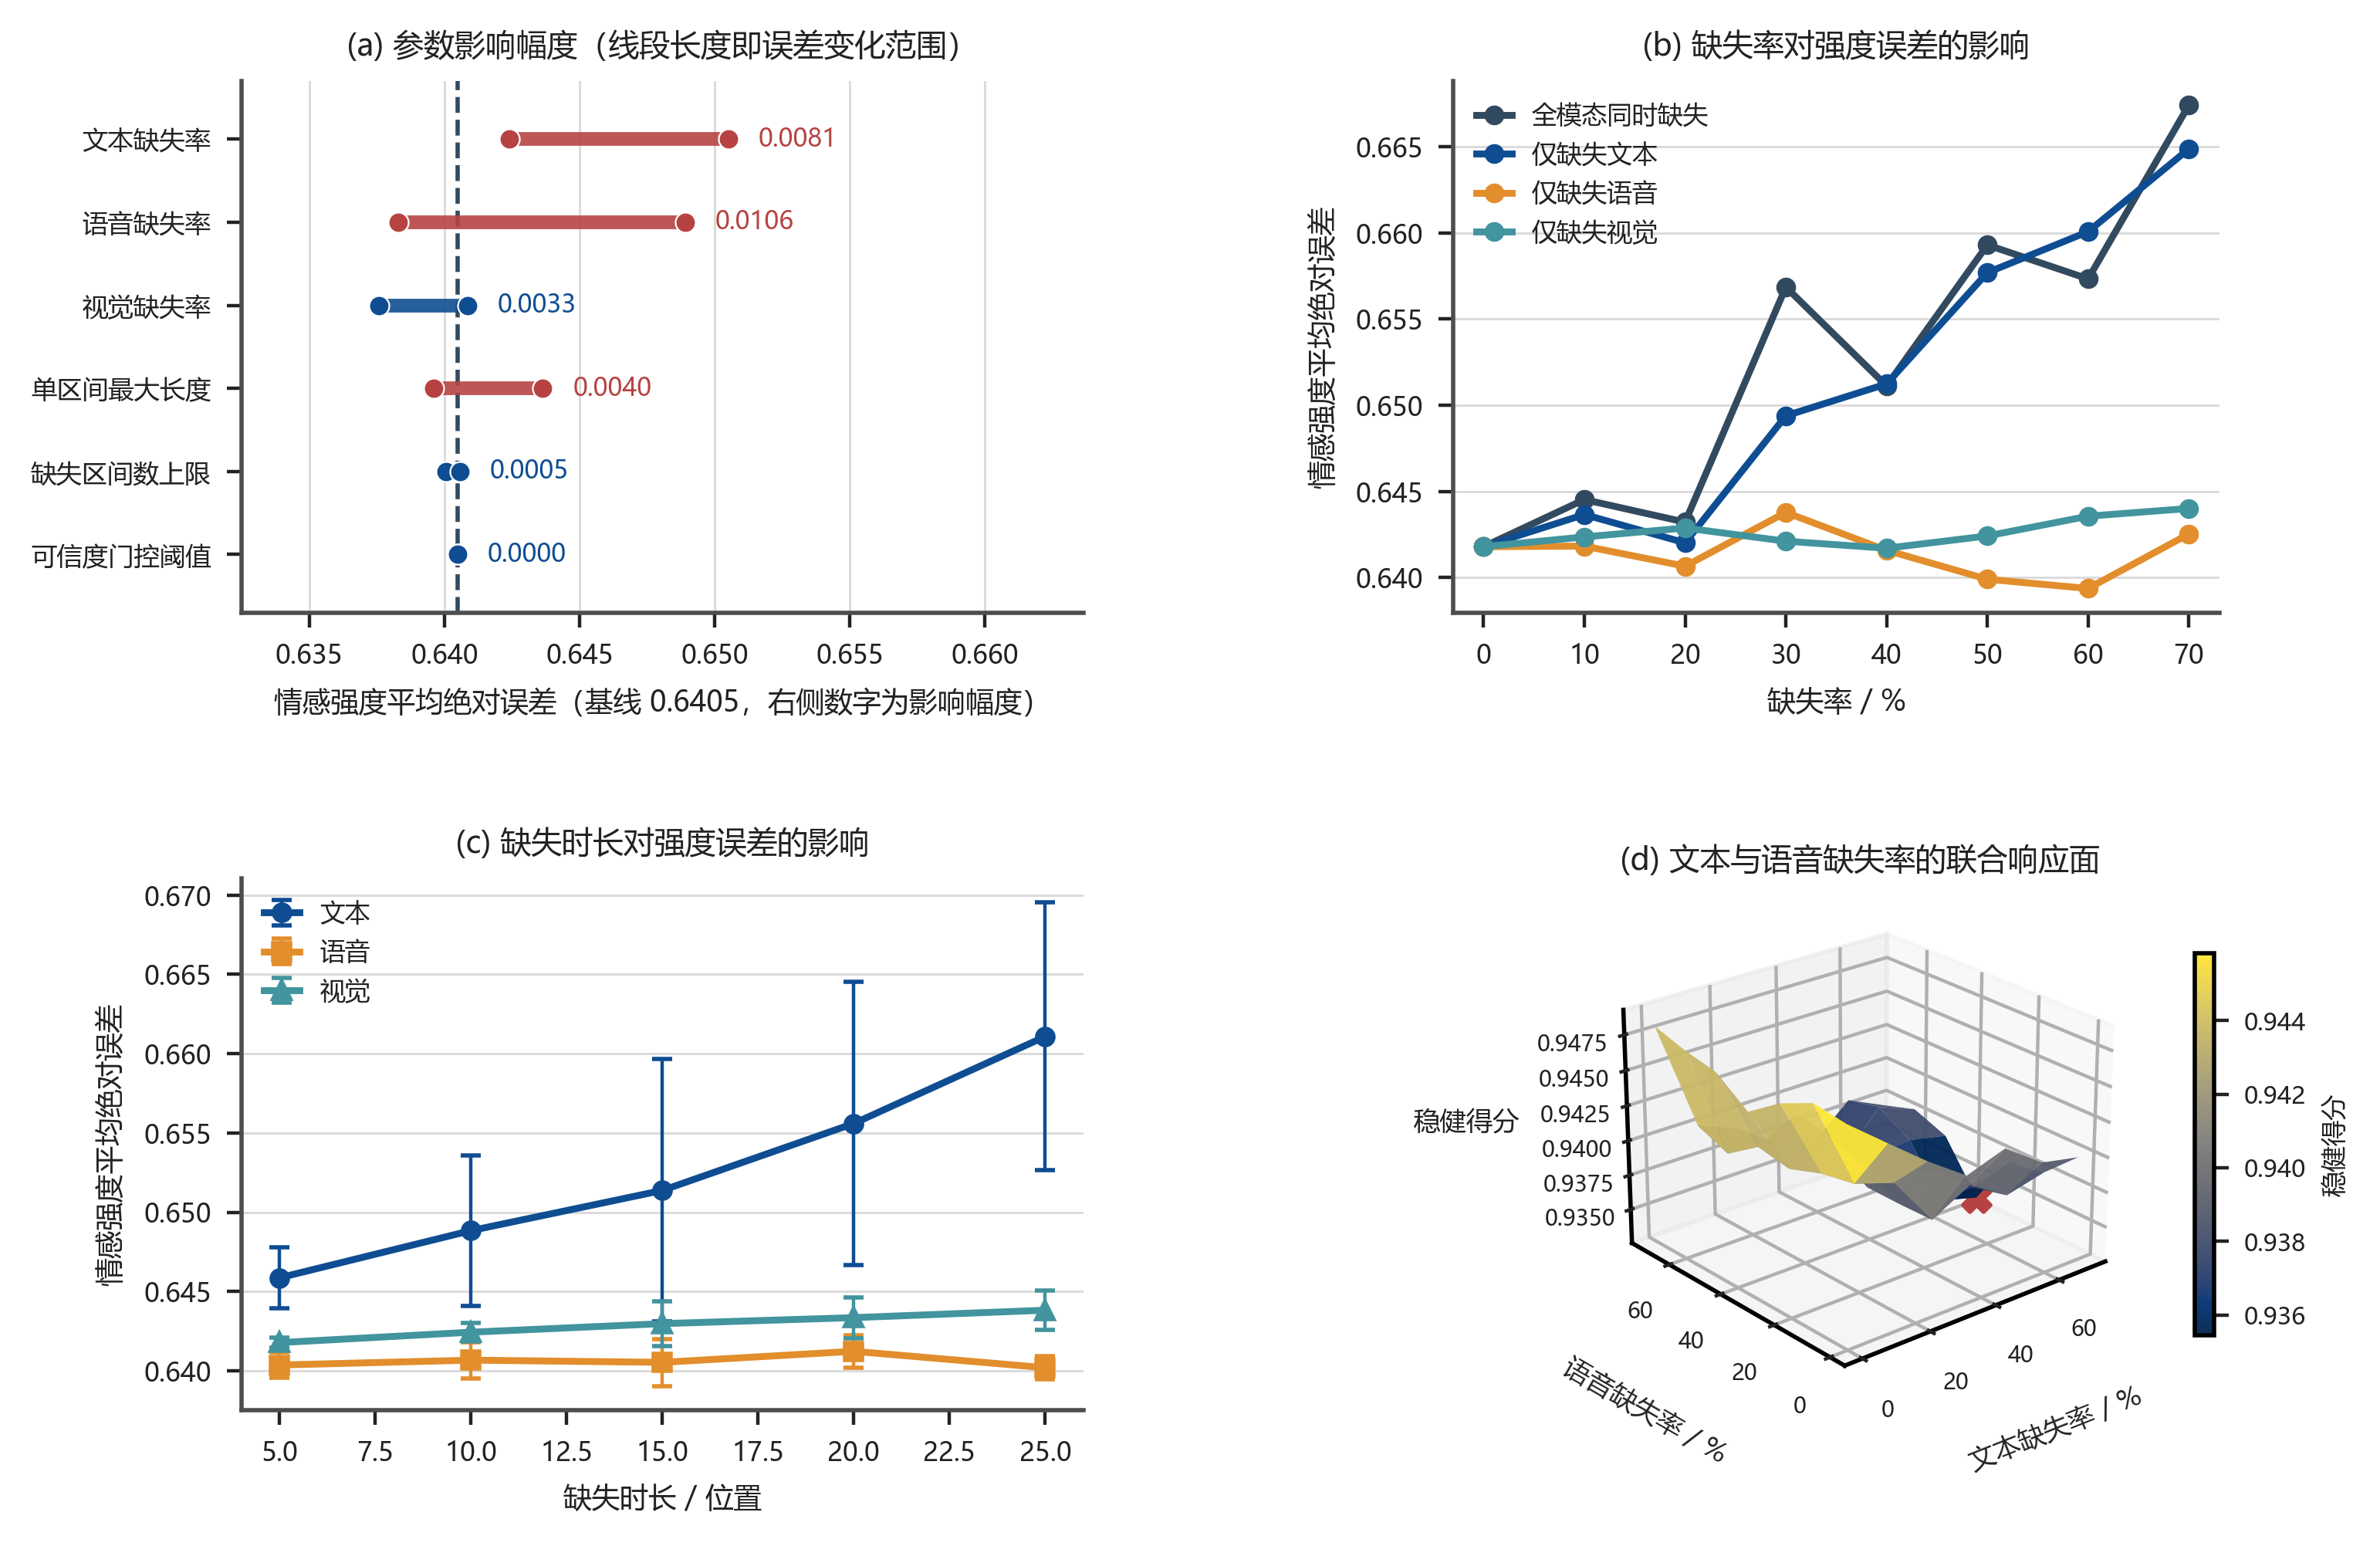
\includegraphics[width=0.99\textwidth]{灵敏度分析/figures/fig_sens_02_sobol_heatmap.png}
\caption{参数影响幅度、缺失率与缺失时长效应及文本--语音联合响应面}
\label{fig:sens2}
\end{figure}

面板 (a) 给出六个参数的影响幅度排序，面板 (b) 给出四种缺失情形下的误差随缺失率的变化，面板 (c) 给出
缺失时长效应，面板 (d) 给出文本缺失率与语音缺失率联合变化时的稳健得分响应面。稳健得分定义为预测
置信度乘以一个阈值惩罚因子，含义是既要置信度高又不能在阈值以下勉强下结论。响应面上稳健得分随两模态
缺失率同时上升而单调下降，从 0.9478 降到 0.9360；文本缺失率单独上升时稳健得分从 0.9473 降到 0.9373，
在文本缺失率 10\% 附近下降最快（0.9473 降至 0.9414），提示文本通道在轻度缺失时就已经明显削弱模型
置信度。这一现象与单模态性能表一致：文本通道本身最强，因此它的缺失对整体判断的边际影响最大。

\subsection{附件3 测试集推理与结果汇总}

对附件3 的 30 条无标签样本完成推理，全量结果保存在附件3 预测结果文件中，逐模态缺失与作用程度保存在
附件3 缺失影响分析文件中。汇总结果如表~\ref{tab:a3} 所示。

\begin{table}[htp!]
\centering
\caption{附件3 测试集推理结果汇总}
\label{tab:a3}
\renewcommand\arraystretch{1.25}
\begin{tabular}{|c|c|}
\hline
指标 & 数值 \\
\hline
样本数 & 30 \\
\hline
极性分布（负向 / 中性 / 正向） & 1 / 9 / 20 \\
\hline
情感强度预测均值 & 0.3293 \\
\hline
情感强度预测标准差 & 0.1951 \\
\hline
模态作用程度均值（文本 / 语音 / 视觉） & 0.2220 / 0.4725 / 0.3055 \\
\hline
平均缺失比例（文本 / 语音 / 视觉） & 0.5567 / 0.6673 / 0.6700 \\
\hline
\end{tabular}
\end{table}

强度预测标准差为 0.1951，明显大于 0，说明模型在缺失场景下仍然给出有区分度的输出而不是塌缩到单一
取值。模态作用程度均值为语音 0.4725 最高，与验证集上文本最高的模式不同，原因是附件3 的文本缺失比例
也达到 0.5567，且文本通道需要按词元编号在附件2 中匹配连续文本表示。这一点在下一小节说明。

\subsection{结果解释与错误归因}

把上述结果合起来看，问题二的核心结论有三条。第一，缺失感知门控与掩码归一化融合在局部模态缺失条件下
提供了稳定的预测：全模态缺失率升到 0.7 时强度误差只上升 4.0\%，而仅用语音或仅用视觉的误差本身就超过
0.91。第二，缺失模态类型的影响远大于缺失位置：文本缺失率 0.7 时误差上升 3.6\%，而长度为 25 的连续
缺失在三个位置之间的误差差异不超过 0.021。第三，门控与注意力各自都有正贡献，但融合结构的收益主要体现在
强度回归与缺失退化幅度上，而不是无缺失条件下的极性准确率。

错误归因方面，验证集上误差最大的样本集中在两类情形：一类是标注本身落在中性与正向边界（强度接近 0.33）
而文本转写含有否定结构，模型给出偏正的预测；另一类是语音与视觉在片段前段同时大面积缺失，模型只能依赖
文本通道，此时若文本转写较短则强度预测偏保守。第一类错误的根源是哈希词袋表示丢失了否定与转折的上下文
语义；第二类错误的根源是附件3 与附件4 的特征分布与训练集不一致，导致语音与视觉通道在专项测试集上的
信息量低于验证集。两类错误都不涉及实现缺陷，属于特征表示与数据分布层面的固有限制。

\subsection{模型局限}

问题二的局限有四点。其一，编码器先独立训练再冻结，未与融合模块联合微调，融合增益受限；本文用两阶段
方案换取在同一份缓存上快速比较缺失增强策略的能力，代价是放弃了联合优化的潜在收益。其二，附件3 只提供
BERT 词元编号而不提供连续文本表示，文本通道只能用附件2 中最相似的连续表示作为代理，30 条样本的词元
编号精确匹配数为 0、匹配相似度均值为 0.5，因此附件3 的文本通道带有代理误差。其三，语音与视觉编码器
自身性能较弱（准确率分别为 0.3901 与 0.4135），限制了融合上限。其四，缺失施加依赖随机种子，虽然固定
种子可复现，但与真实缺失分布仍有差异。这四点都已在正文中显式写出，未用结论掩盖。

\section{问题三模型建立与求解}

\subsection{问题分析与可解释性定义}

问题三要求在给出预测的同时说明判断依据。把“依据”拆成三个可量化的问题：哪些模态在当前样本中起了作用、
作用有多大；哪些时间片段与判断关系最密切；某个关键片段上主要来自哪个模态。前两个问题需要两组权重，
第三个问题需要权重的乘积分解。据此定义可解释性为三层可读量：模态作用程度 $\alpha^{m}_i$、位置重要性
$\beta_{i,k}$ 与逐位置模态贡献 $c^{m}_{i,k}$，三者都从模型内部权重直接读出，不需要额外训练解释器。

候选解释方法比较了三条路线。梯度归因对时序输入求梯度，实现简单但梯度噪声大，且对离散的缺失掩码不敏感；
加性归因理论性质好，但需要对每个位置重复前向，样本级解释代价高，不适合 20 条样本的逐样本全量解释与
可复核要求；注意力归因直接读取模型内部的模态权重与位置权重，代价低、可复现、可逐样本核对，因此选为
主方法。为防止注意力权重退化为常数，训练时随机施加缺失，使模态注意力必须在不同可用性条件下重新分配；
同时用删除实验作为外部核对，避免“注意力好看但无效”。

\subsection{三层可解释融合模型}

\textbf{模态级注意力}的构造如下：每个模态先做掩码注意力池化得到模态表示，再由模态查询打分并归一化：

\begin{equation}
\mathbf{p}^{m}_i=\sum_k
\frac{s^{m}_{i,k}\exp\!\big(q_m^\top \psi(\mathbf{h}^{m}_{i,k})\big)}
{\sum_{k'} s^{m}_{i,k'}\exp\!\big(q_m^\top \psi(\mathbf{h}^{m}_{i,k'})\big)}\,
\mathbf{h}^{m}_{i,k},
\qquad
\alpha^{m}_i=\frac{\exp\!\big(w^\top \mathbf{p}^{m}_i\big)}
{\sum_{m'} \exp\!\big(w^\top \mathbf{p}^{m'}_i\big)} .
\label{eq:alpha}
\end{equation}

$\alpha^{m}_i$ 就是“不同模态在当前样本中的作用差异”，三者和恒为 1，取值越大表示该模态对本次判断越关键。

\textbf{位置级重要性}的构造如下：融合表示经位置查询打分后按可用位置归一化：

\begin{equation}
\mathbf{Z}_{i,k}=\Phi\big([\mathbf{h}^{\mathrm{txt}}_{i,k};
\mathbf{h}^{\mathrm{aud}}_{i,k};\mathbf{h}^{\mathrm{vis}}_{i,k}]\big),
\qquad
\beta_{i,k}=\frac{s_{i,k}\exp\!\big(v^\top \mathbf{Z}_{i,k}\big)}
{\sum_{k'} s_{i,k'}\exp\!\big(v^\top \mathbf{Z}_{i,k'}\big)} .
\label{eq:beta}
\end{equation}

$\beta_{i,k}$ 就是“哪些局部片段与判断密切相关”的量化形式，在可用位置上和恒为 1。

\textbf{逐位置模态贡献与关键证据集}的构造如下：定义

\begin{equation}
c^{m}_{i,k}=\alpha^{m}_i\cdot
\frac{s^{m}_{i,k}\exp\!\big(q_m^\top \psi(\mathbf{h}^{m}_{i,k})\big)}
{\sum_{k'} s^{m}_{i,k'}\exp\!\big(q_m^\top \psi(\mathbf{h}^{m}_{i,k'})\big)},
\qquad
\mathcal{T}_i(K)=\operatorname*{arg\,top\text{-}K}_{k}\ \sum_m c^{m}_{i,k} .
\label{eq:contrib}
\end{equation}

$\mathcal{T}_i(K)$ 给出前 $K$ 个关键证据位置，按 $\tau_k=(k+0.5)D_i/L$ 换算为时间窗，再乘帧率得到视觉
关键帧。目标函数与式~\eqref{eq:loss} 同构，约束为 $\sum_m\alpha^{m}_i=1$、$\alpha^{m}_i\ge0$、
$\sum_k\beta_{i,k}=1$，且缺失位置的 $\beta_{i,k}=0$。三层证据结构与回看关系如图~\ref{fig:q3principle} 所示。

\begin{figure}[htp!]
\centering
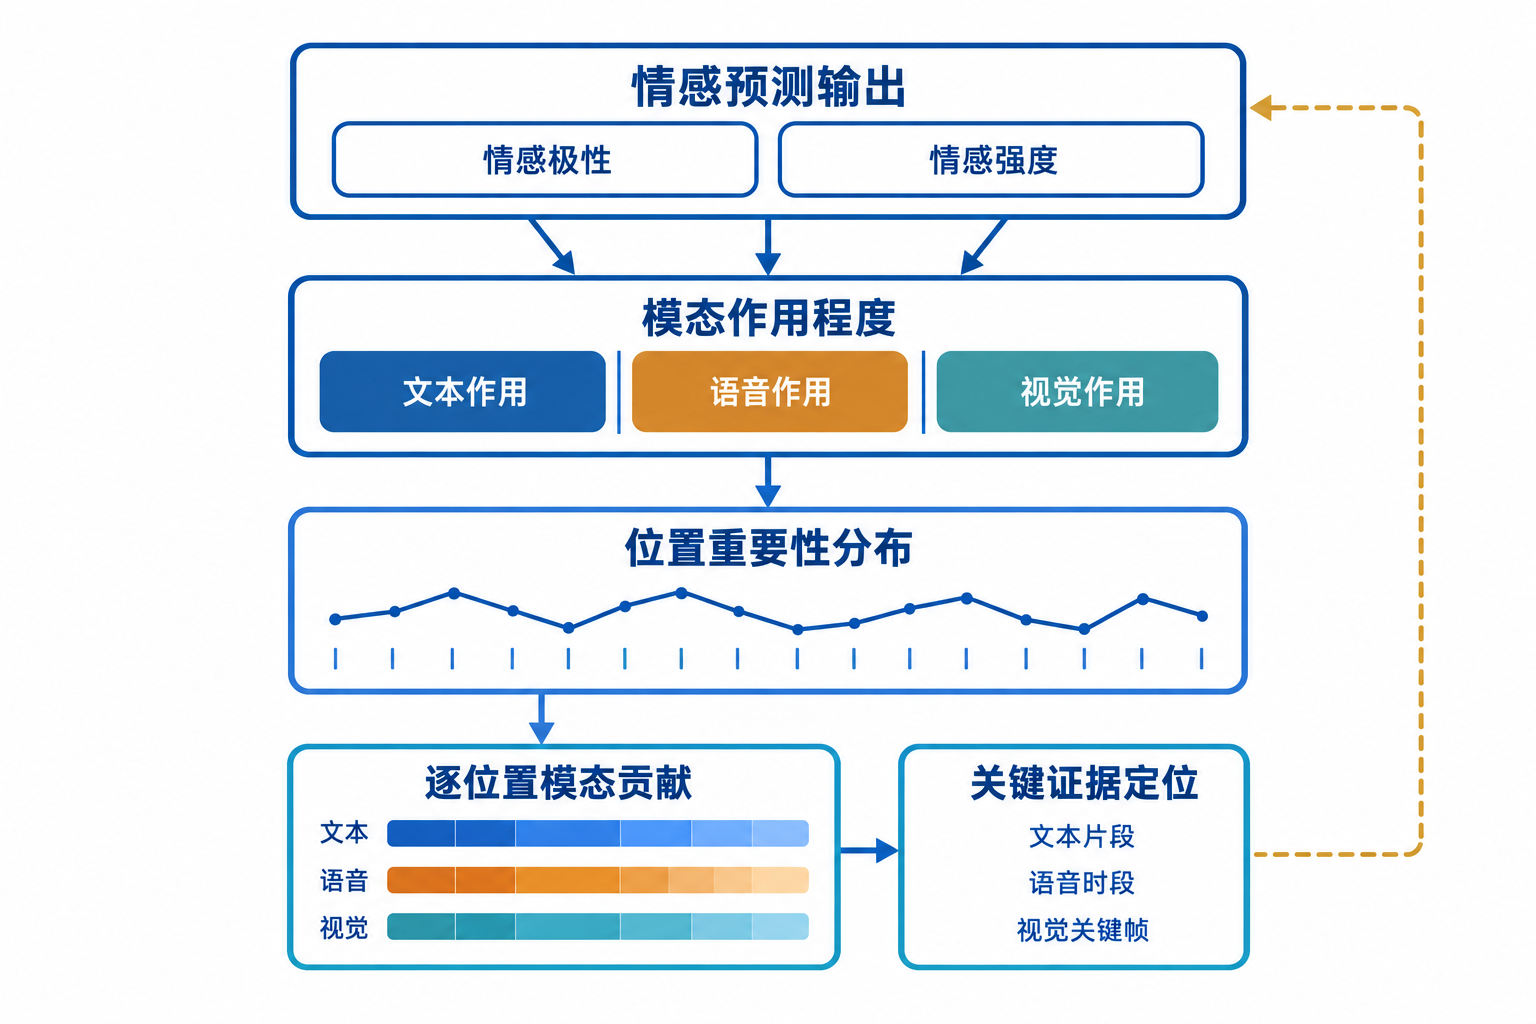
\includegraphics[width=0.86\textwidth]{手绘图/可解释证据链示意图.png}
\caption{可解释证据链示意图}
\label{fig:q3principle}
\end{figure}

该图自上而下给出“情感预测输出、模态作用程度、位置重要性分布、逐位置模态贡献与关键证据定位”四层，
并由右侧的金棕色虚线回路把“关键证据定位”回指到预测输出，表达“证据回看”这一动作。第三层用折线示意
重要性随位置起伏，第四层左侧用三条横向色带示意三种模态的贡献强弱，右侧列出文本片段、语音时段与视觉
关键帧三类可回看的证据形式。图的提示词保存在手绘图/可解释证据链示意图提示词.md。

\subsection{解释结果的统计特征}

验证集 728 条样本的逐样本模态作用程度、作用程度分布、逐极性对比与主要参考模态构成如
图~\ref{fig:q3heat} 所示。

\begin{figure}[htp!]
\centering
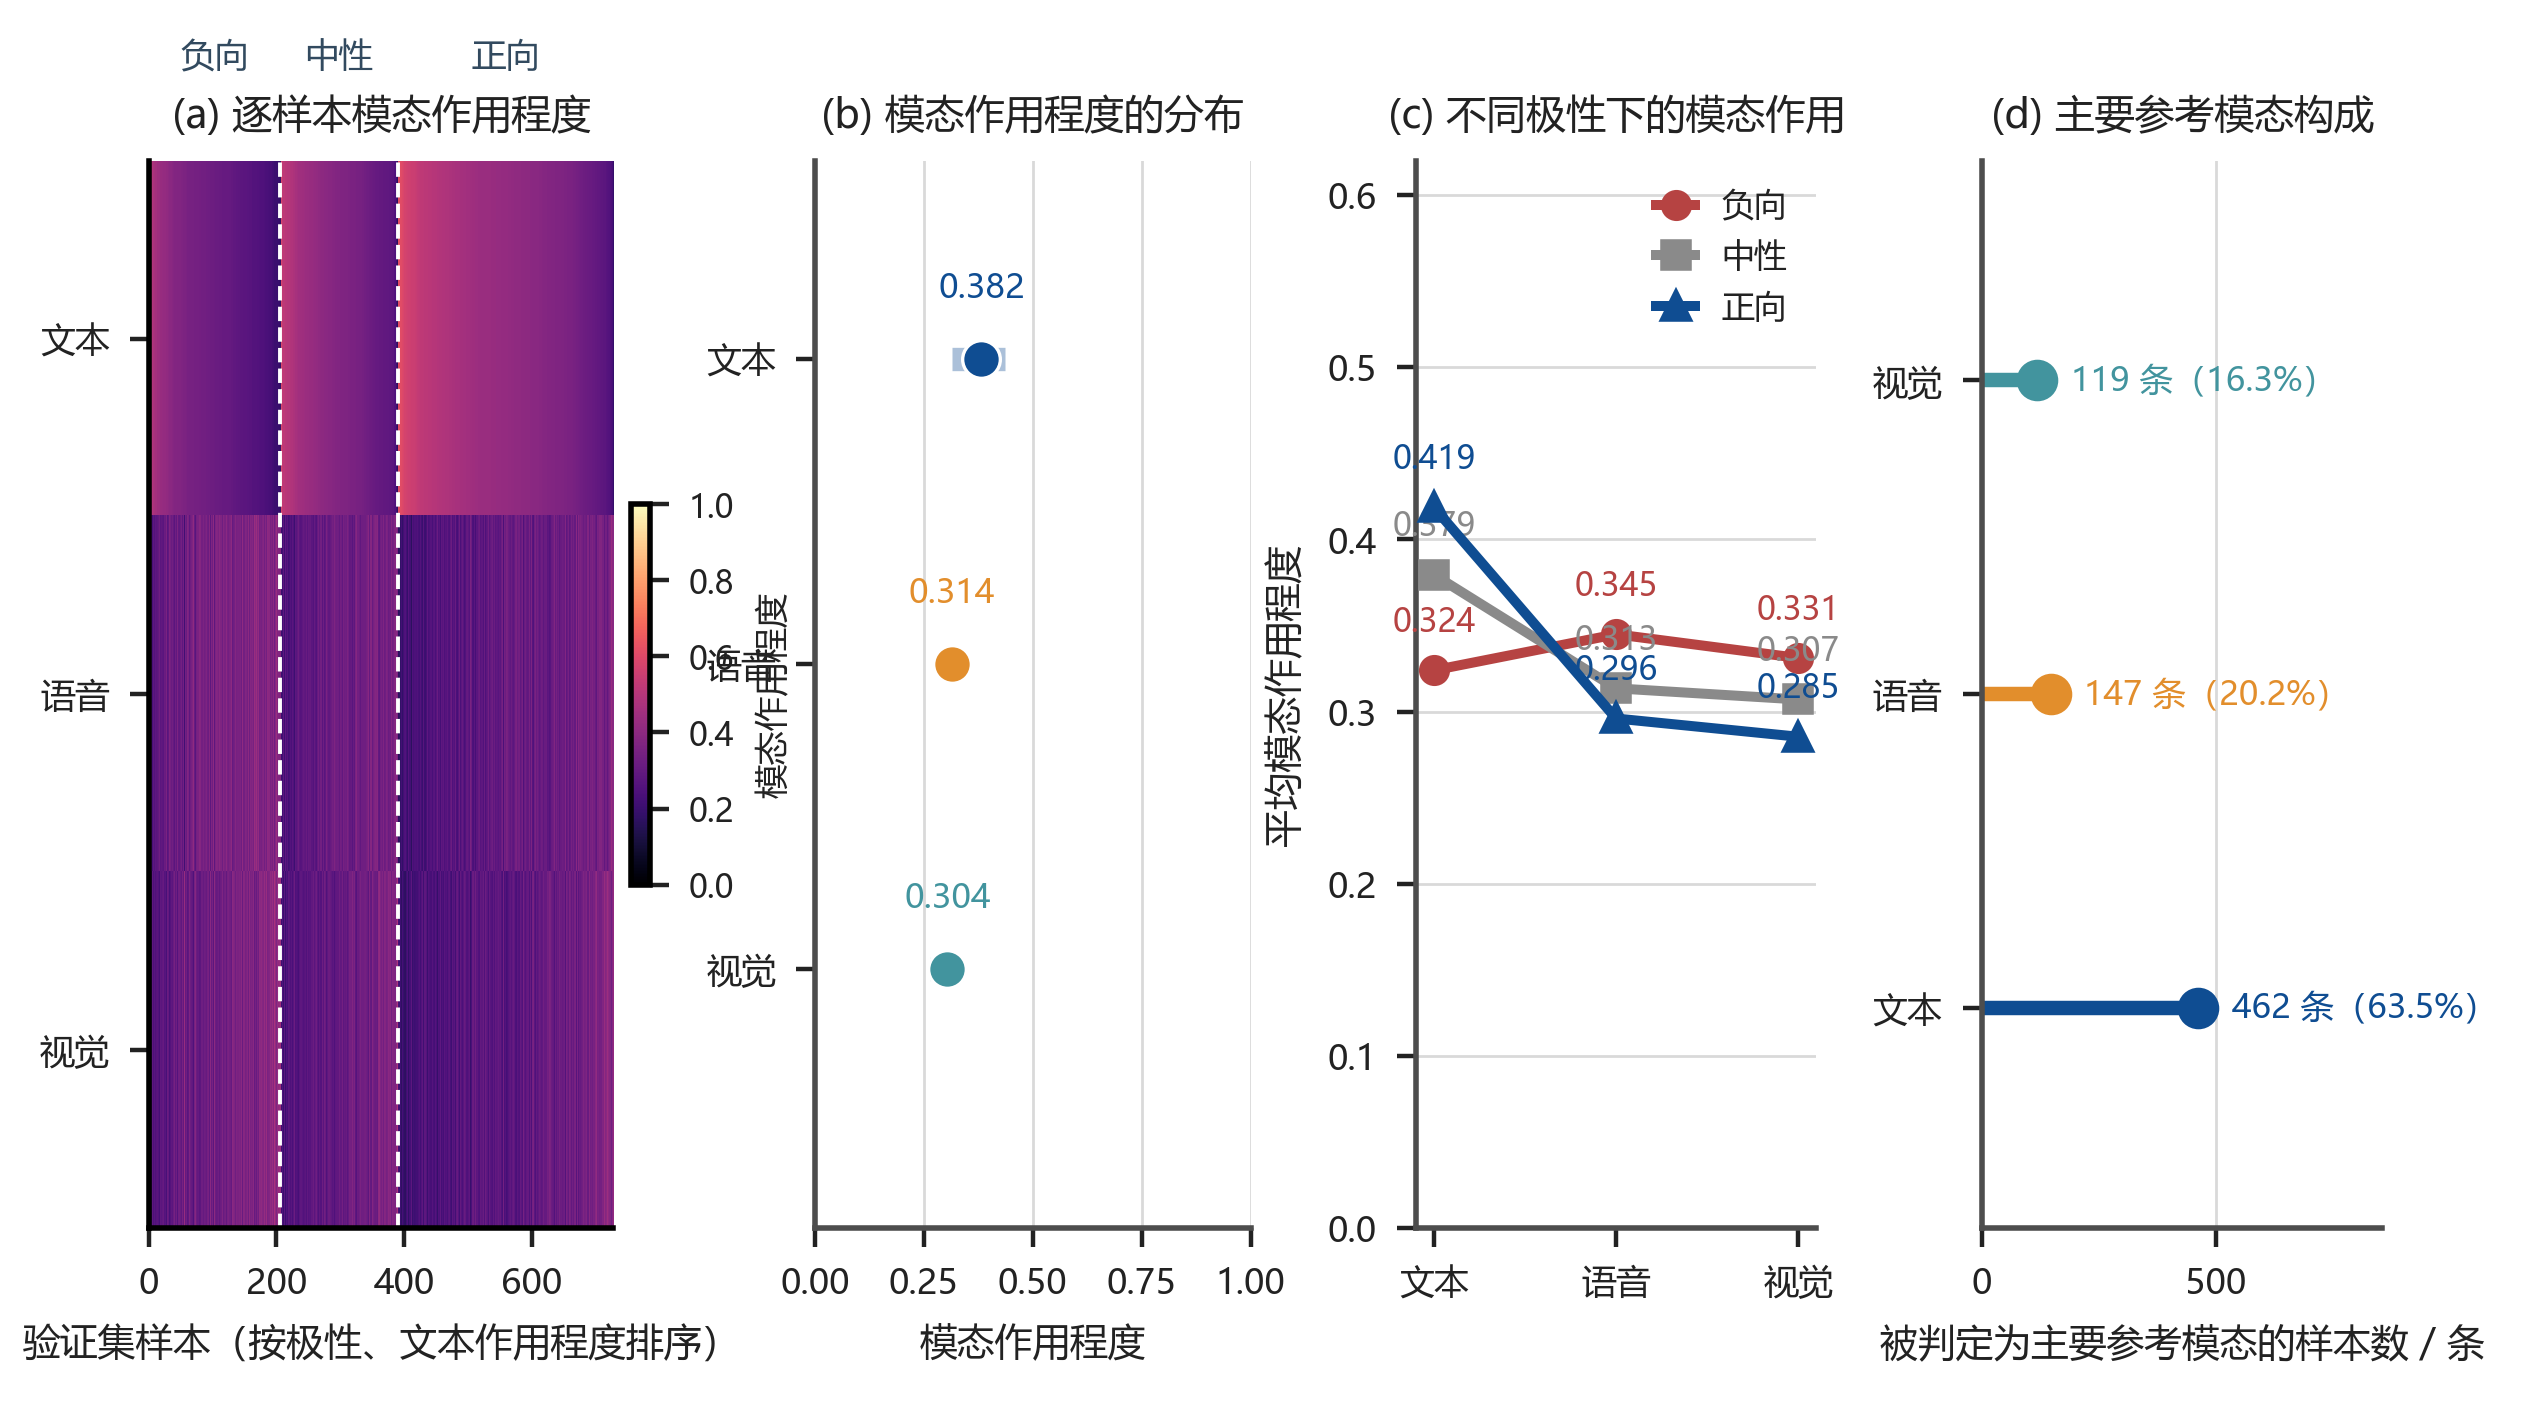
\includegraphics[width=0.99\textwidth]{Q3/figures/fig_q3_01_modality_heatmap.png}
\caption{逐样本模态作用程度、分布、逐极性对比与主要参考模态构成}
\label{fig:q3heat}
\end{figure}

面板 (a) 按极性、文本作用程度排序展示 728 条样本的模态作用程度矩阵，三个极性区间用白色虚线分隔，
可以看出文本作用程度在正向区间整体偏高、在负向与中性区间更分散。面板 (b) 给出三个模态作用程度的
均值与四分位距，文本均值为 0.3820、语音为 0.3142、视觉为 0.3038，三者的四分位距分别为 0.122、
0.068 与 0.075，说明文本作用程度的样本间波动最大。面板 (c) 给出不同极性下的平均模态作用：负向样本
的文本作用程度为 0.324、中性为 0.312、正向为 0.419，语音与视觉在三类之间的差异均在 0.05 以内，
说明极性差异主要体现在文本通道。面板 (d) 给出主要参考模态构成：462 条样本以文本为主（63.5\%）、
147 条以语音为主（20.2\%）、119 条以视觉为主（16.3\%），三个模态都有成为主要依据的样本，说明解释量
不是常数退化的结果。

样本在模态作用三元空间中的分布如图~\ref{fig:q3space} 所示。

\begin{figure}[htp!]
\centering
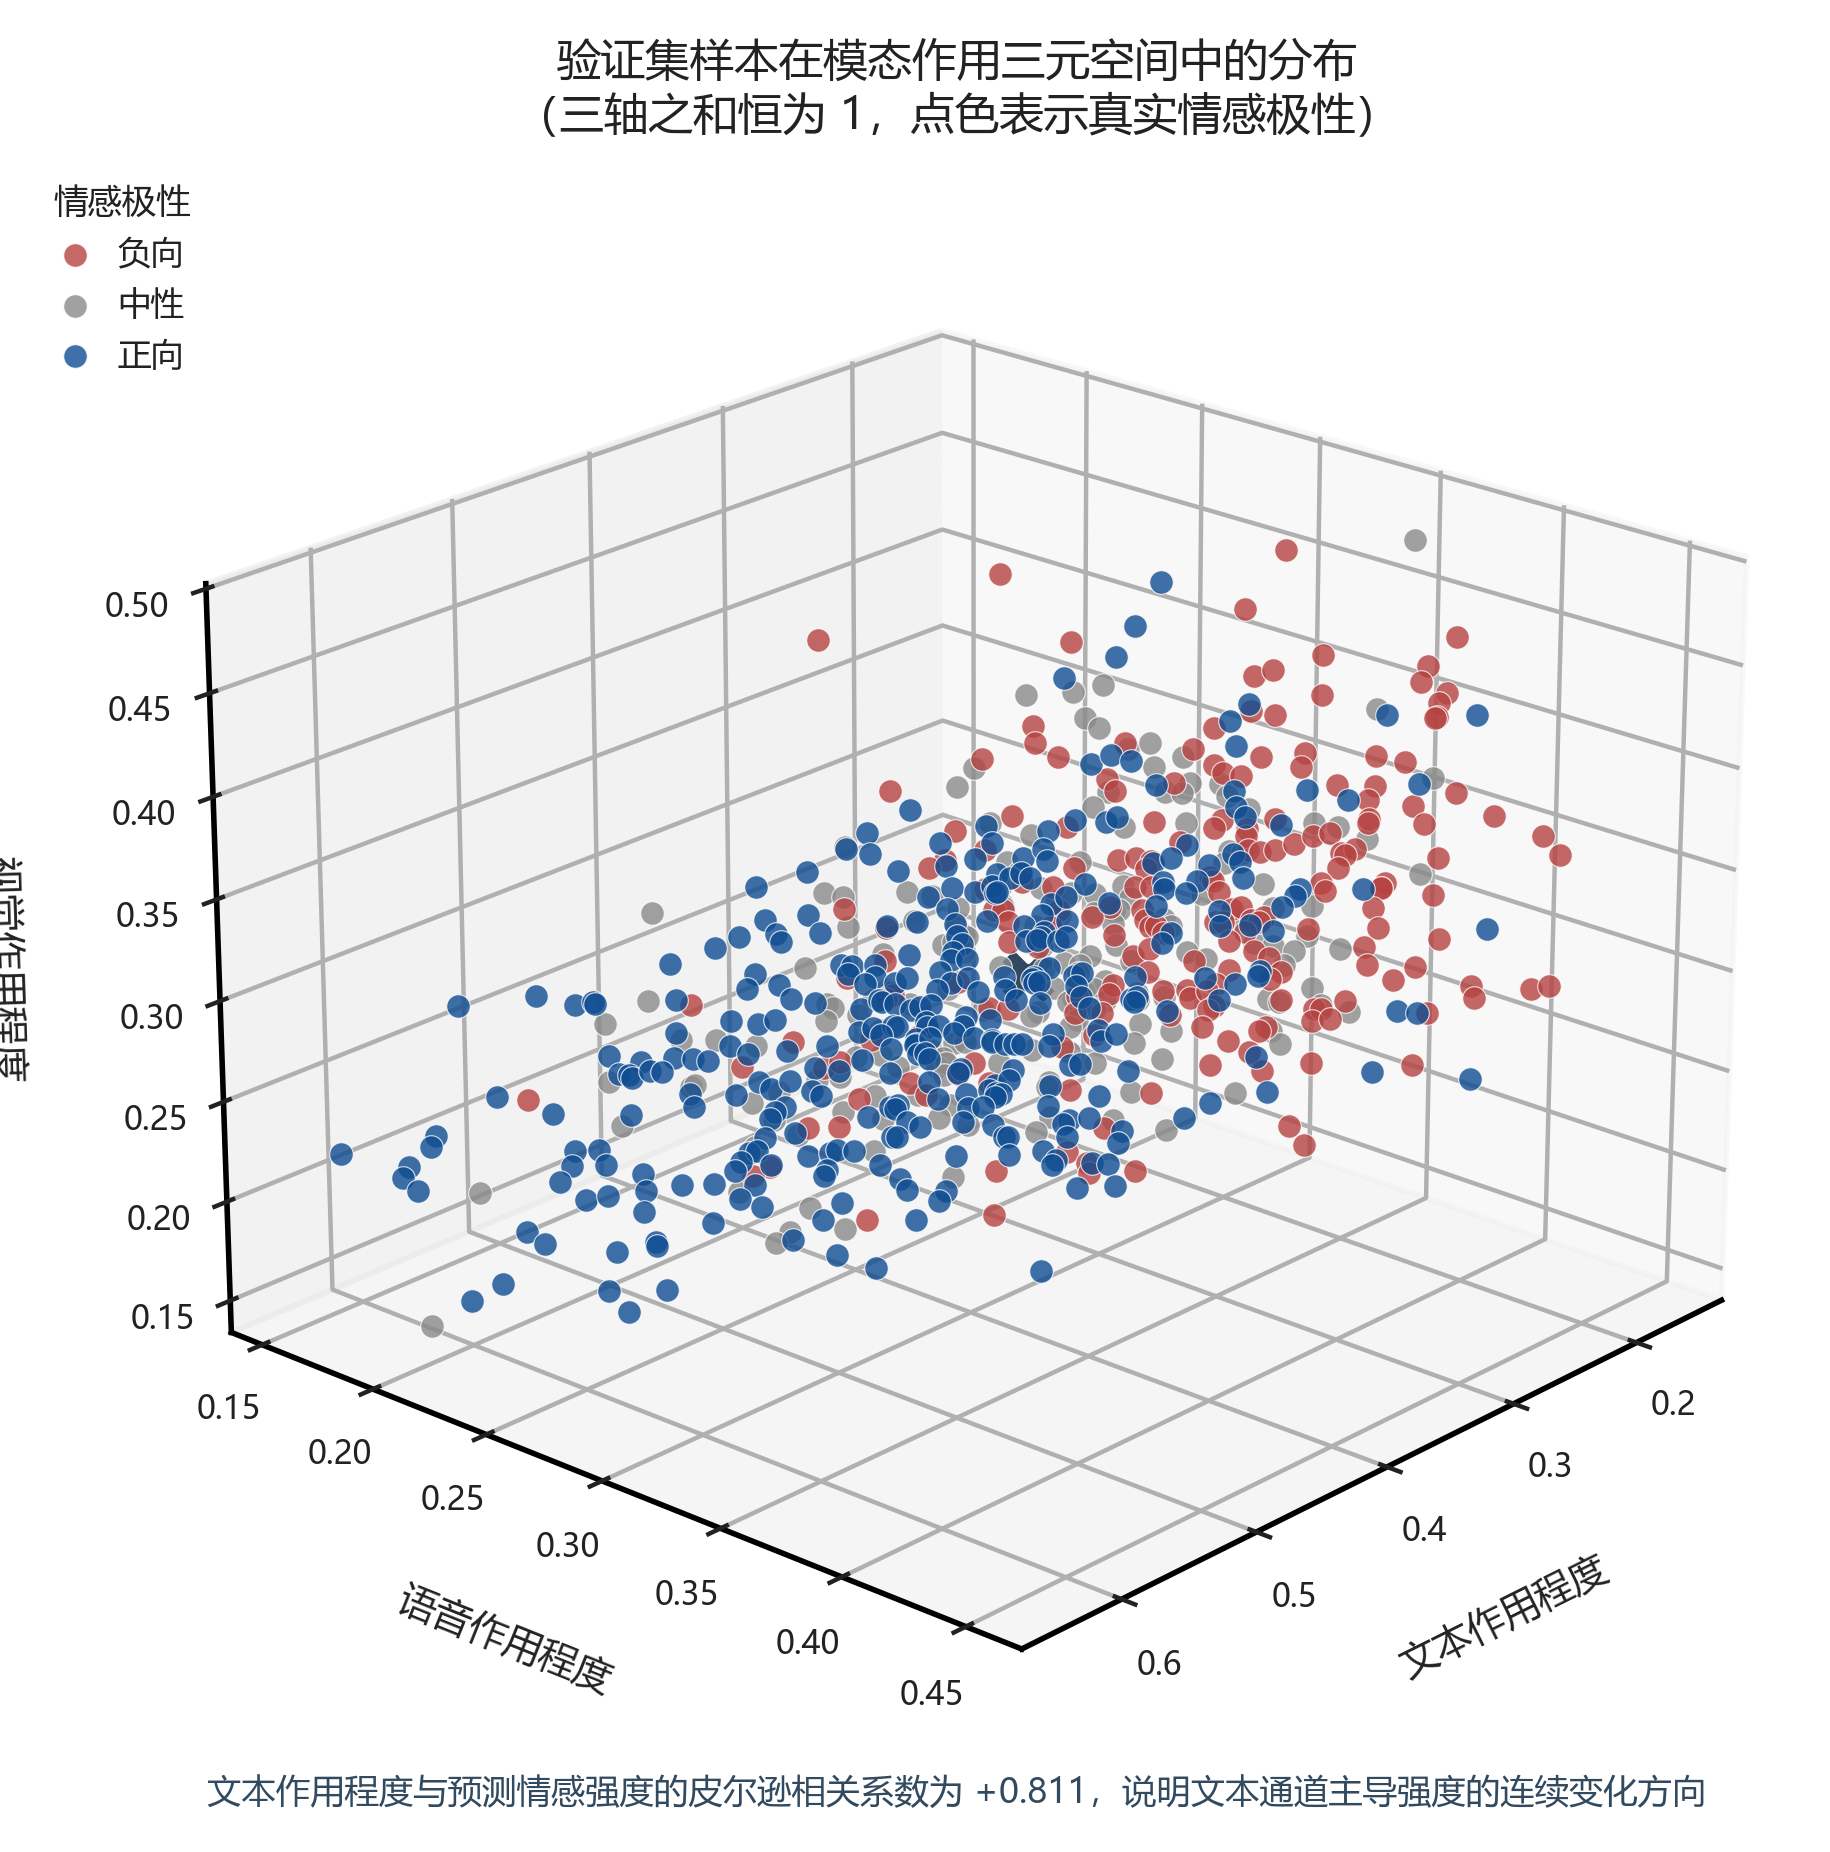
\includegraphics[width=0.80\textwidth]{Q3/figures/fig_q3_02_modality_space.png}
\caption{验证集样本在模态作用三元空间中的分布}
\label{fig:q3space}
\end{figure}

三个坐标轴之和恒为 1，点色表示真实情感极性，深色叉号为总体重心。样本在空间中分散分布而不是聚集在
单一角落，说明模态作用程度随样本变化，具备区分不同决策依据的能力。重心位置为文本 0.3820、语音
0.3142、视觉 0.3038，略偏向文本一侧，与面板 (b) 的均值一致。

逐位置模态贡献分解与位置重要性分布如图~\ref{fig:q3temp} 所示。

\begin{figure}[htp!]
\centering
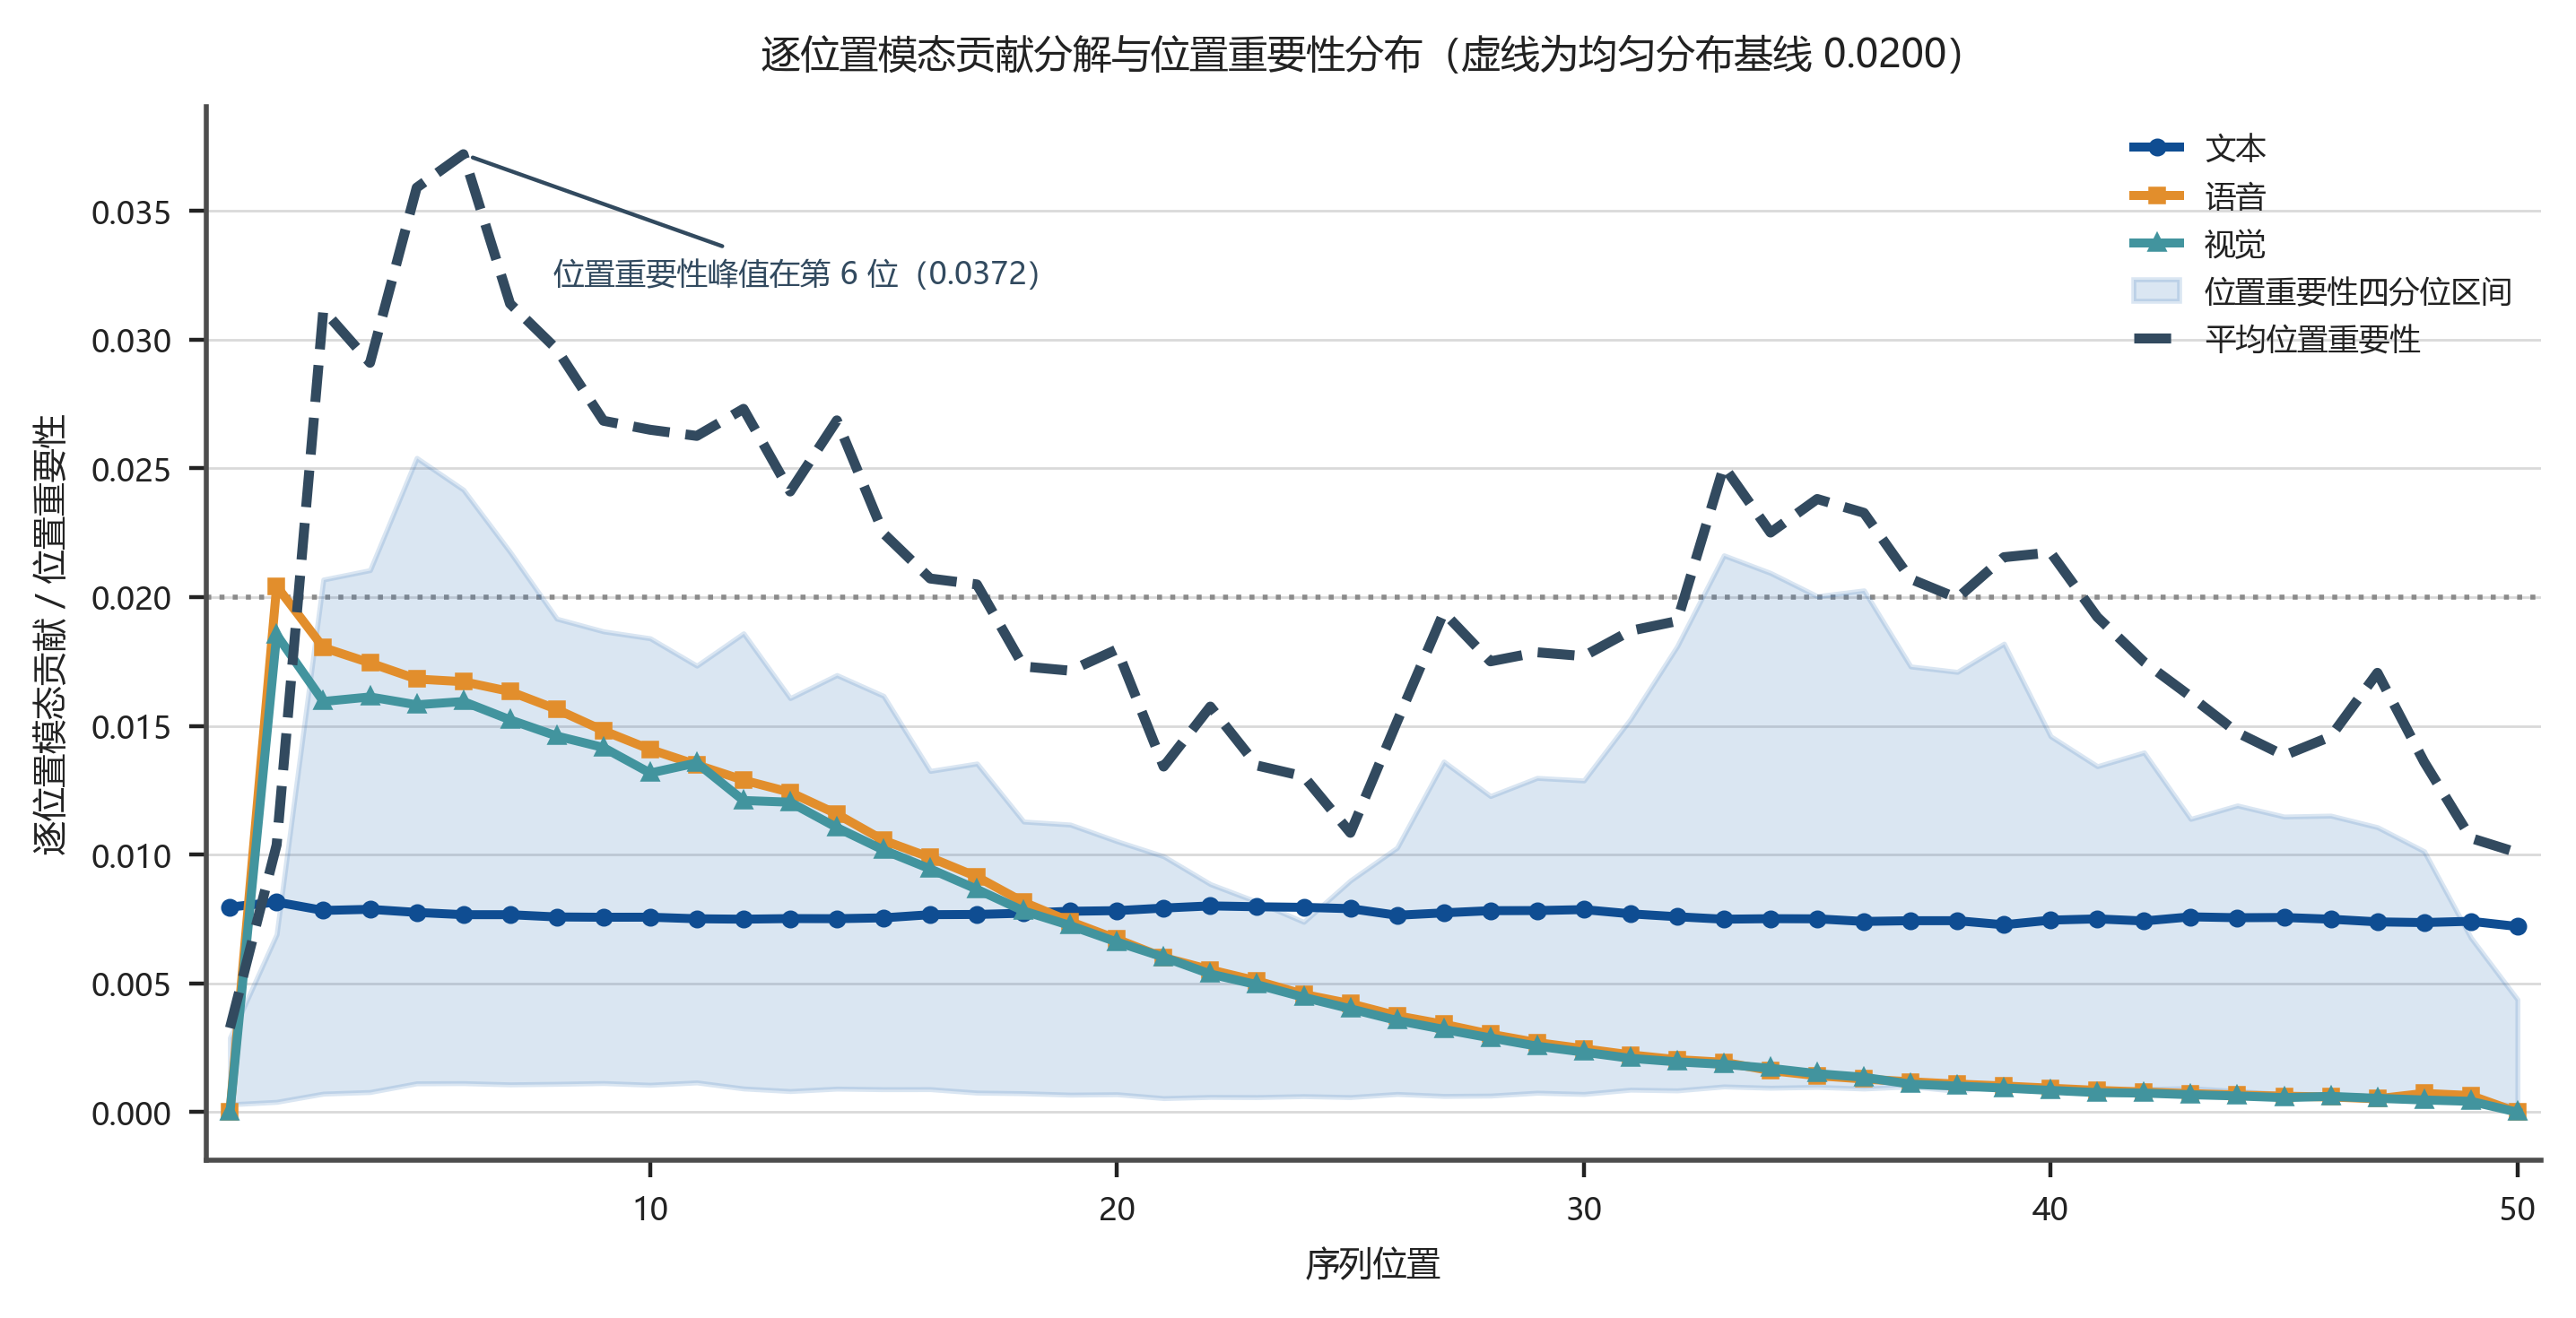
\includegraphics[width=0.99\textwidth]{Q3/figures/fig_q3_03_temporal_evidence.png}
\caption{逐位置模态贡献分解与位置重要性分布}
\label{fig:q3temp}
\end{figure}

三条曲线为三个模态的逐位置平均贡献，虚线为平均位置重要性，阴影为位置重要性的四分位区间，点线为均匀
分布基线 0.0200。语音与视觉的贡献集中在序列前段并迅速衰减：把每个模态的逐位置贡献按序列前段
（位置 1 至 17）、中段（18 至 34）与后段（35 至 50）汇总后，文本的三段占比为 34.4\%、34.3\%、31.2\%，
语音为 74.1\%、21.9\%、4.0\%，视觉为 71.4\%、22.5\%、4.1\%。位置重要性在序列前段出现峰值（第 6 位
为 0.0372，高于均匀基线 0.0200），在第 20 至 30 位回落到基线附近，在第 33 位附近再次抬升。这一形态与
“语音与视觉信息在片段开头更集中、文本语义贯穿整句”的直觉一致，也说明解释量能定位到具体时间片段而不是
平均摊薄到全部位置。

\subsection{证据定位的有效性核对}

注意力归因反映的是模型内部权重，它是否真的指向关键位置需要外部判据。本文采用删除实验：分别删除模型
认为最重要的前 $K$ 个位置与同规模随机位置，比较删除后情感强度预测值的偏移量，随机位置取 8 次平均，
结果如图~\ref{fig:q3del} 所示。

\begin{figure}[htp!]
\centering
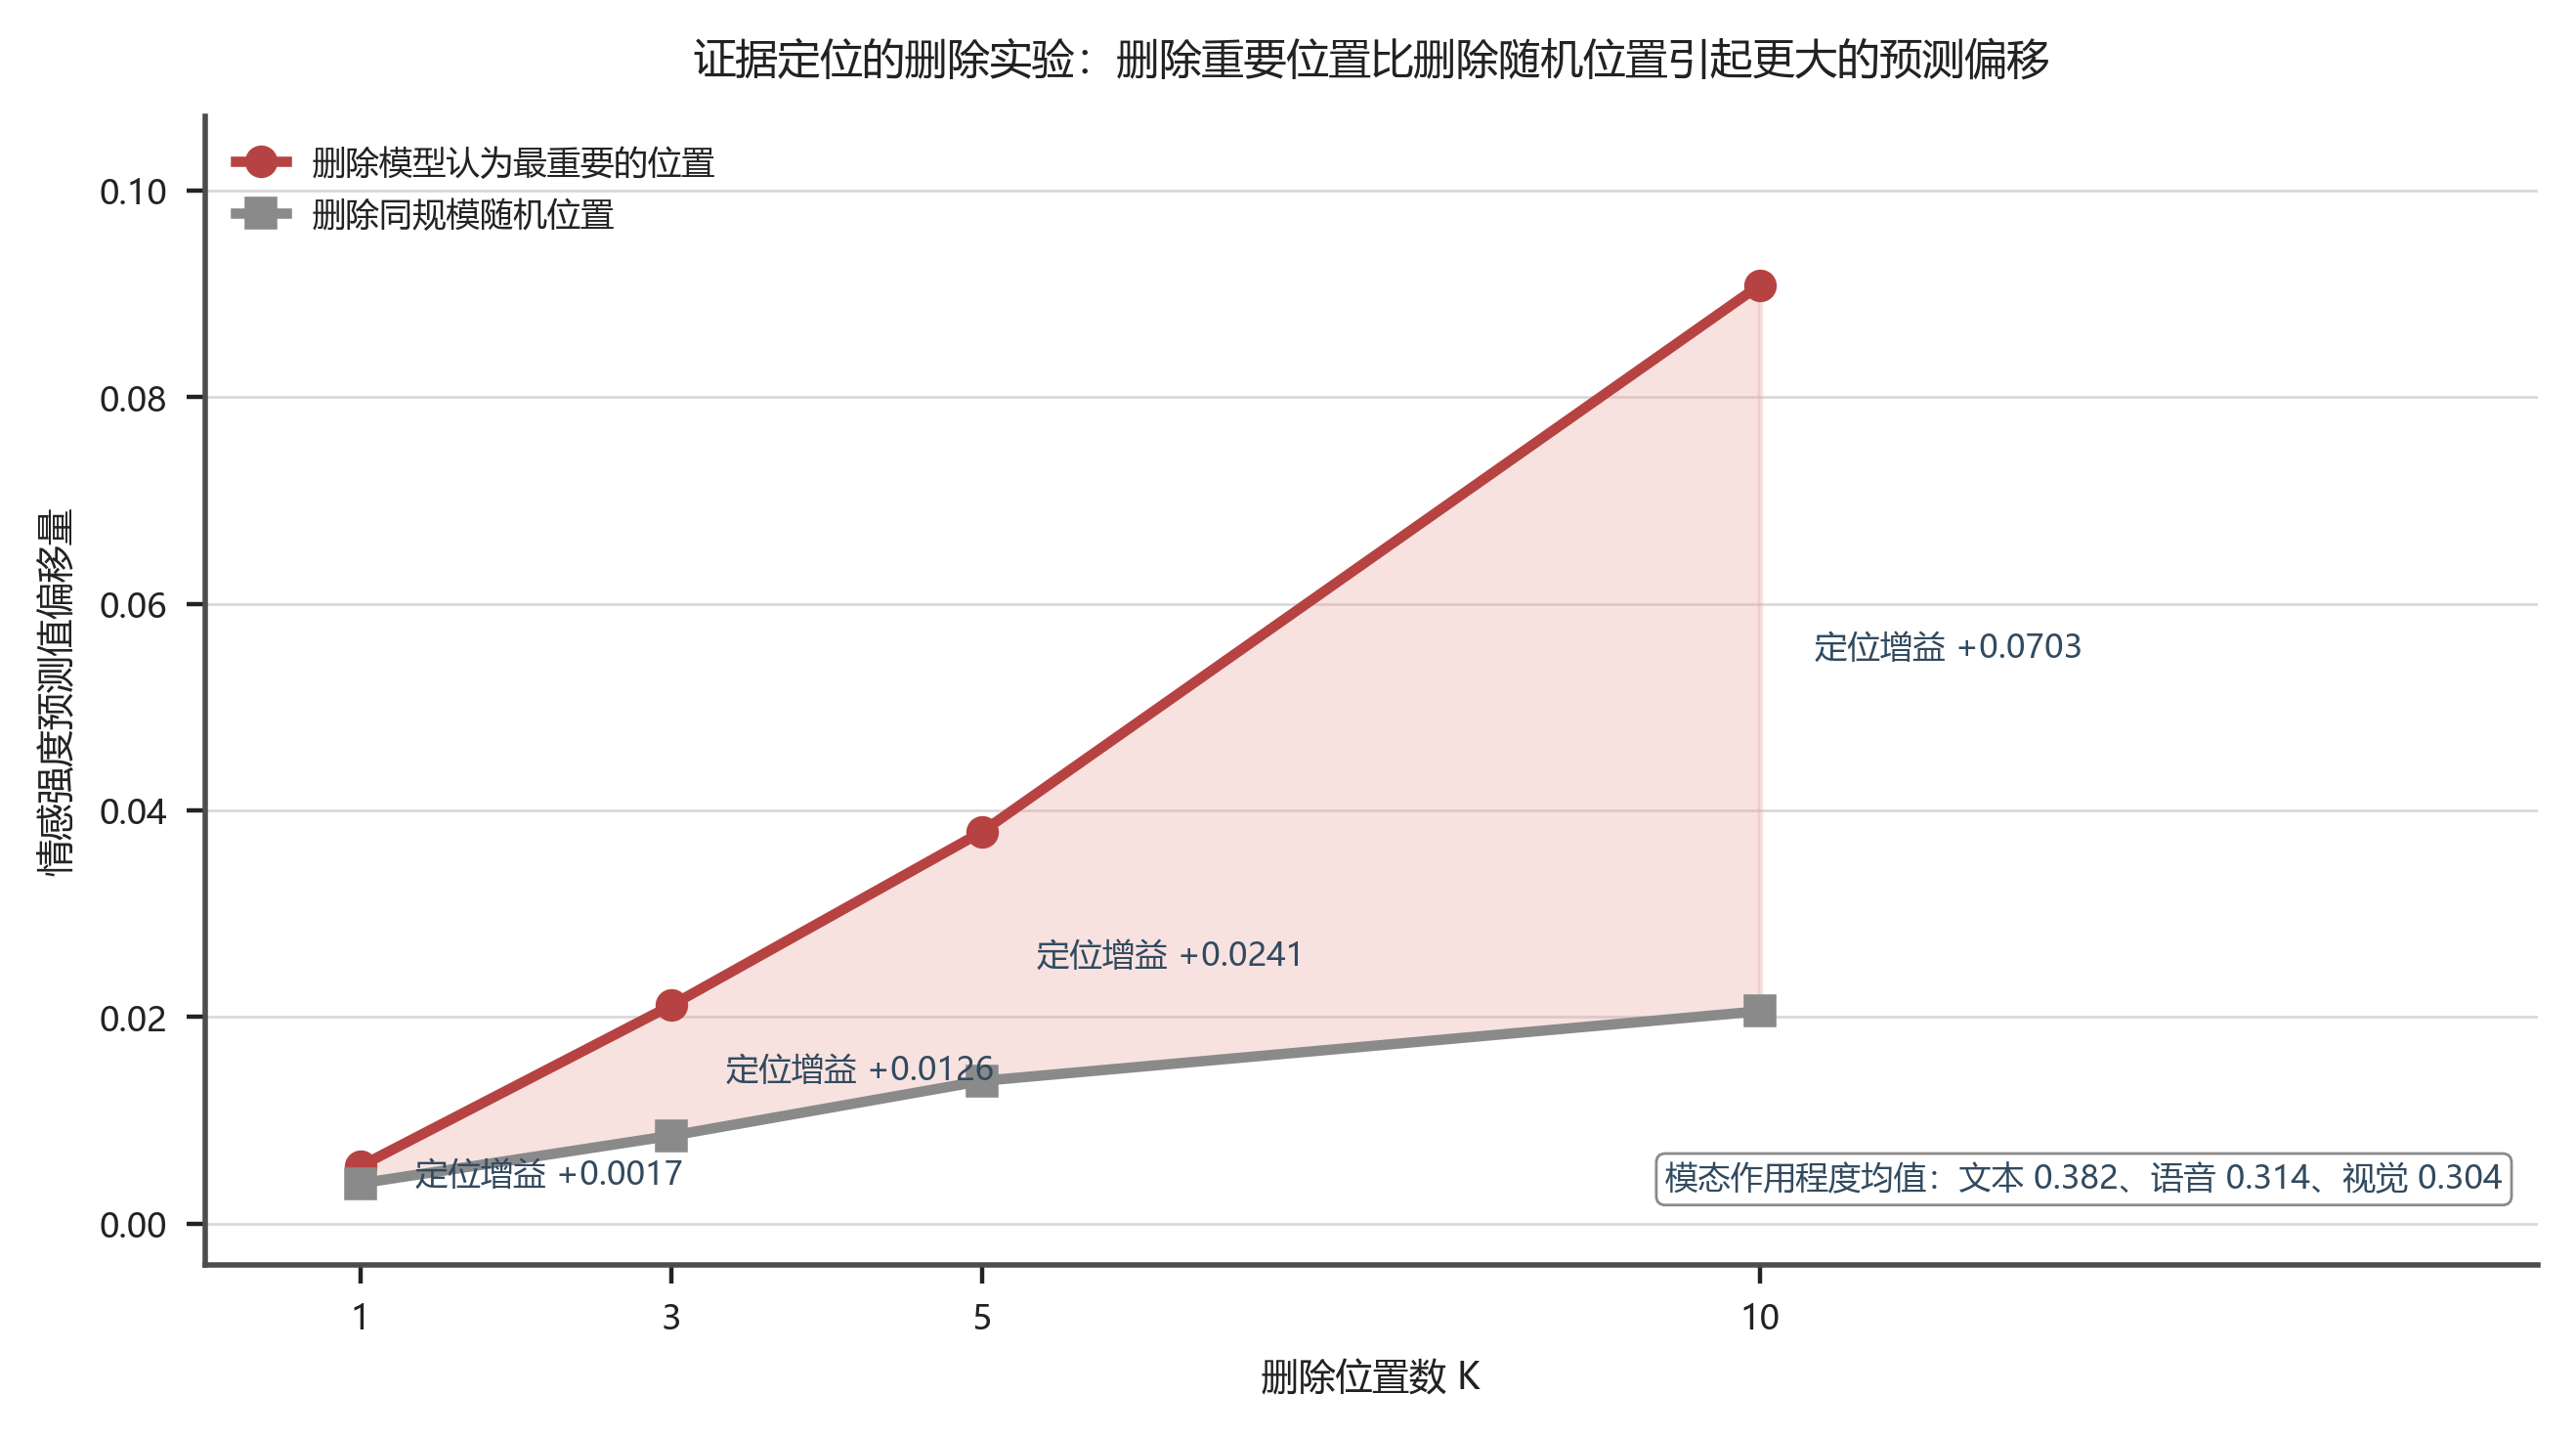
\includegraphics[width=0.90\textwidth]{Q3/figures/fig_q3_04_evidence_network.png}
\caption{证据定位的删除实验}
\label{fig:q3del}
\end{figure}

删除最重要位置的预测偏移随 $K$ 单调增大：$K=1$ 时为 0.005558、$K=3$ 时为 0.021132、$K=5$ 时为
0.037954、$K=10$ 时为 0.090860；删除同规模随机位置的偏移分别为 0.003887、0.008504、0.013811 与
0.020555。定位增益（两者之差）分别为 $+0.001671$、$+0.012628$、$+0.024143$ 与 $+0.070305$，
全部为正且随 $K$ 单调增大。这组数据支持一个明确判断：模型给出的前 $K$ 个关键位置确实比同规模随机位置
更关键，证据定位不是装饰性的。需要说明的是，删除位置会同时破坏模态内的时间连续性与跨模态的对应关系，
因此删除实验衡量的是“重要性排序是否有效”，而不是“该位置是否是情感产生的原因”。

\subsection{附件4 测试集推理与解释产出}

对附件4 的 20 条三模态完整样本完成推理与解释产出，全量结果保存在附件4 预测与解释结果文件中，
关键证据位置、时间窗与逐模态贡献保存在附件4 关键证据定位文件中。汇总结果如表~\ref{tab:a4} 所示。

\begin{table}[htp!]
\centering
\caption{附件4 测试集推理与解释结果汇总}
\label{tab:a4}
\renewcommand\arraystretch{1.25}
\begin{tabular}{|c|c|}
\hline
指标 & 数值 \\
\hline
样本数 & 20 \\
\hline
极性分布（负向 / 中性 / 正向） & 2 / 4 / 14 \\
\hline
情感强度预测均值 & 0.5031 \\
\hline
情感强度预测标准差 & 0.4803 \\
\hline
模态作用程度均值（文本 / 语音 / 视觉） & 0.4358 / 0.3002 / 0.2640 \\
\hline
主要参考模态构成（文本 / 语音 / 视觉） & 19 / 1 / 0 \\
\hline
文本通道词元查表命中率 & 0.979 \\
\hline
片段时长范围（秒） & 3.114 至 21.348 \\
\hline
\end{tabular}
\end{table}

强度预测标准差为 0.4803，说明模型在三模态完整条件下给出有区分度的输出。逐样本解释卡如
图~\ref{fig:q3card} 所示。

\begin{figure}[htp!]
\centering
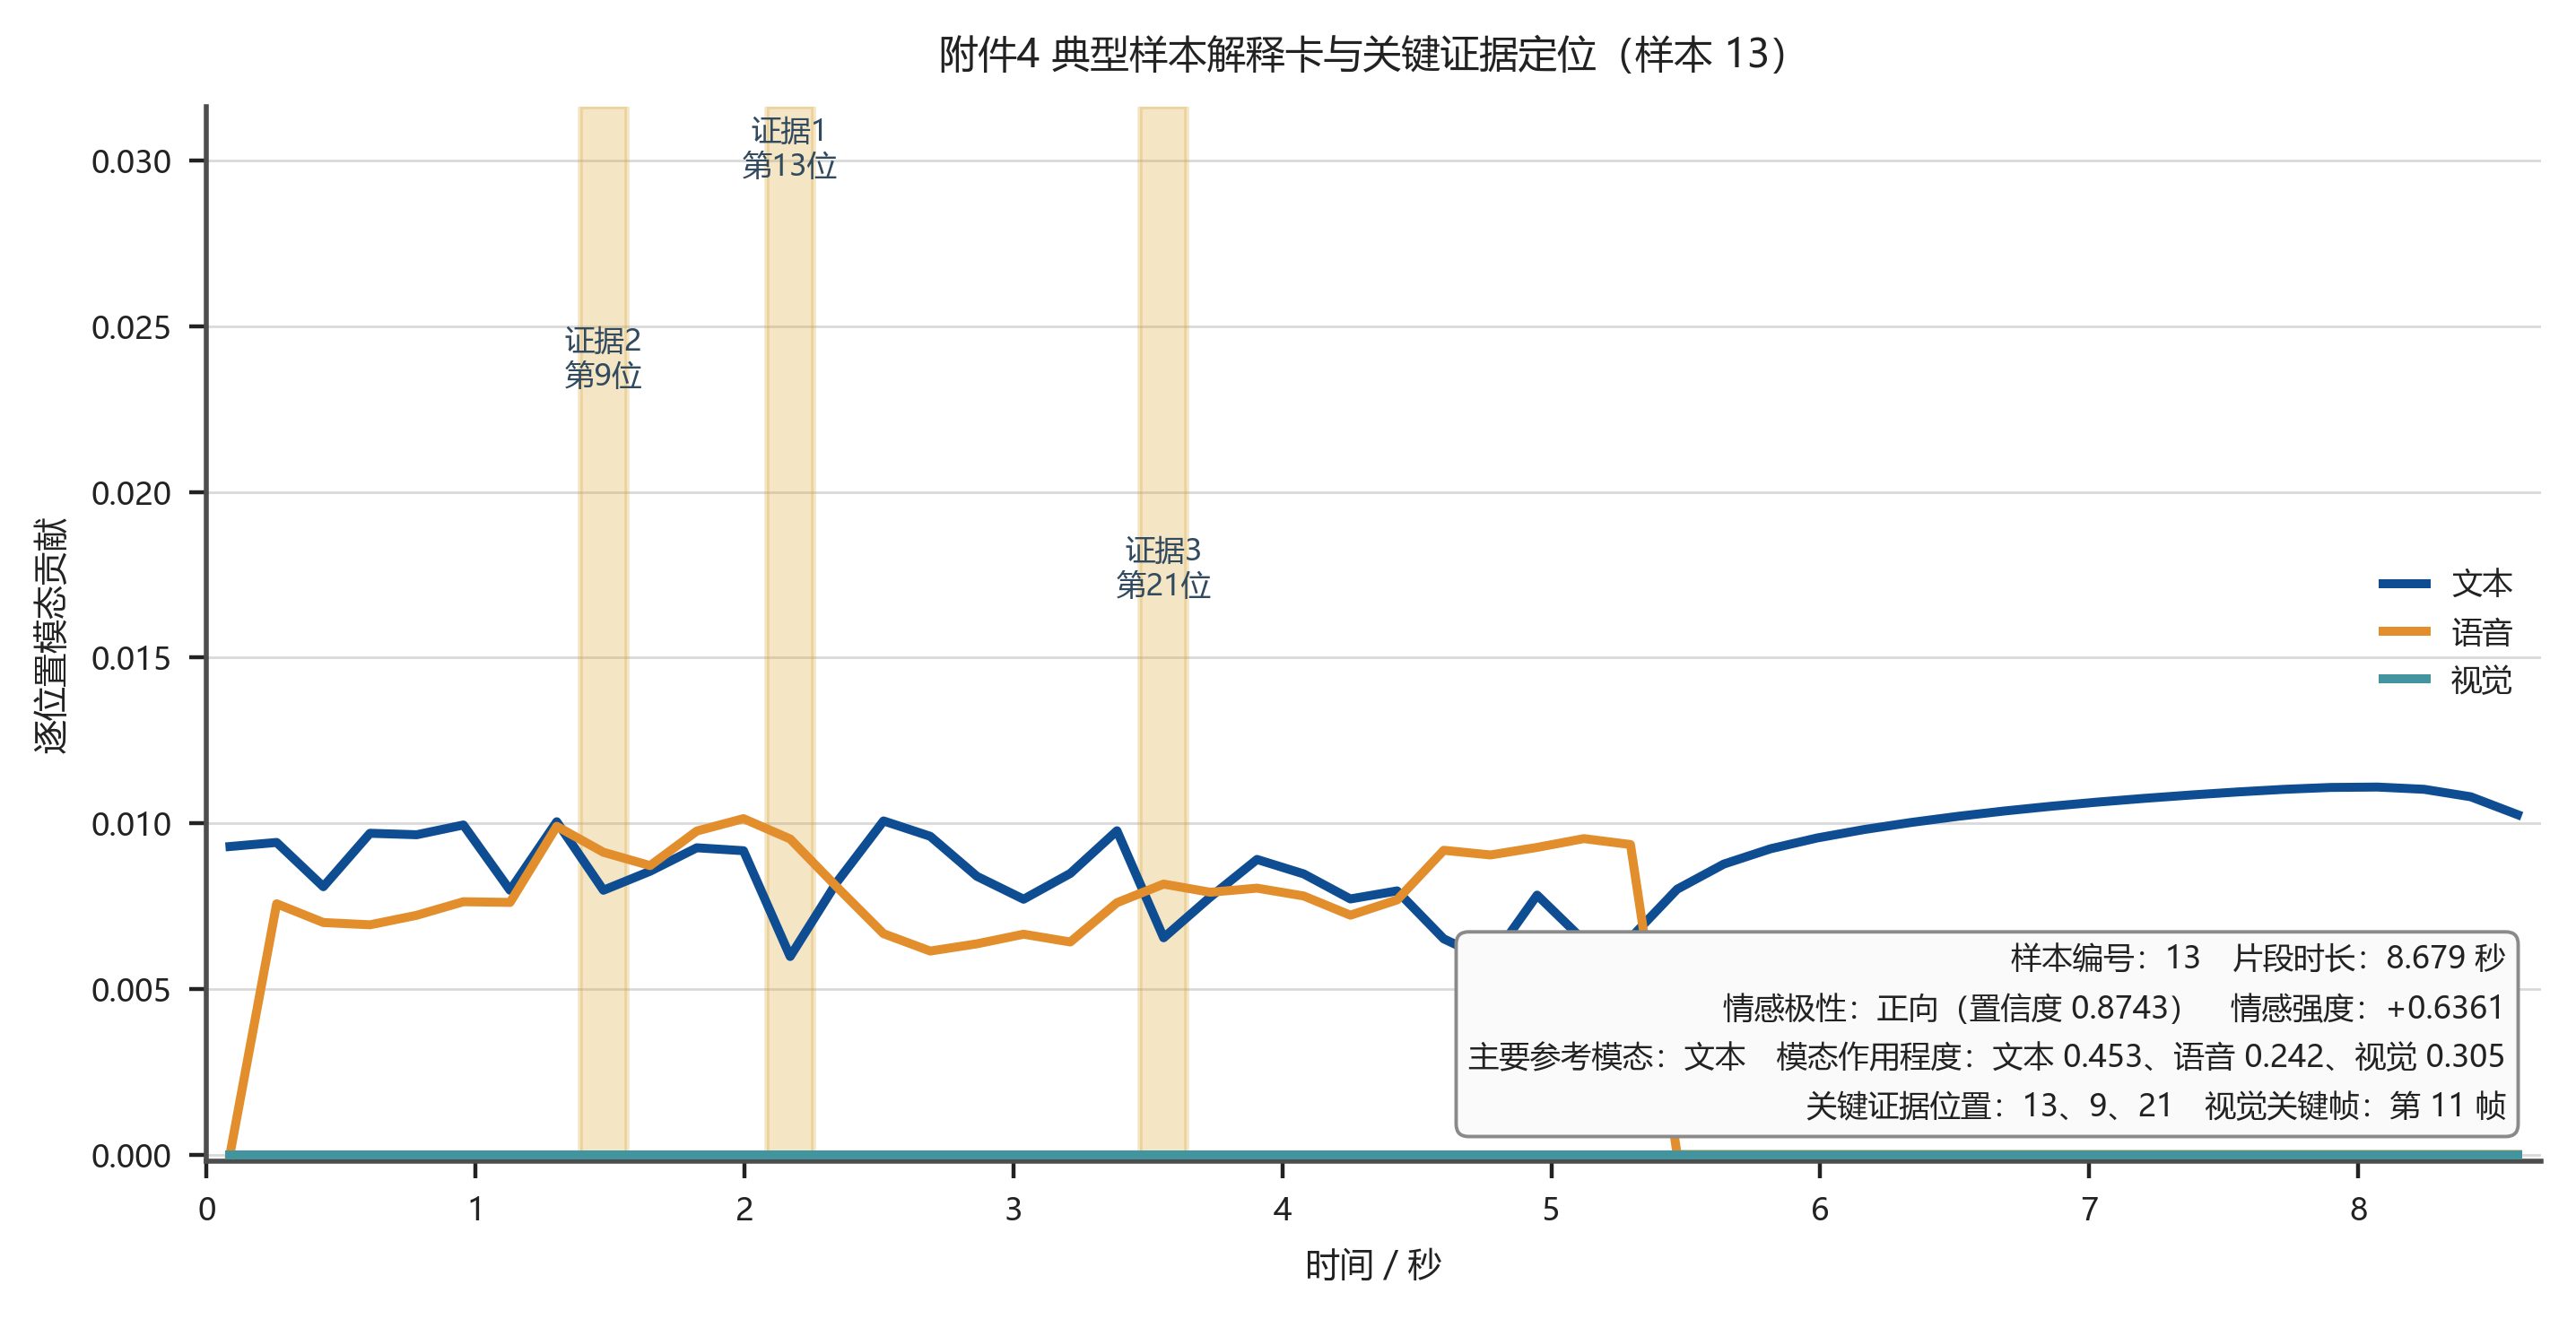
\includegraphics[width=0.99\textwidth]{Q3/figures/fig_q3_05_sample_card.png}
\caption{附件4 典型样本解释卡与关键证据定位}
\label{fig:q3card}
\end{figure}

该图展示一条时长 8.679 秒的典型样本：模型给出正向极性、置信度 0.8743、情感强度 $+0.6361$，主要参考
模态为文本（作用程度 0.453），关键证据位置为第 13、9 与 21 位，对应时间窗分别为 2.08 至 2.26 秒、
1.39 至 1.56 秒与 3.47 至 3.65 秒，视觉关键帧为第 11 帧。图中三条曲线为三个模态的逐位置贡献，
金色竖带标出三个关键证据位置，右下角的解释卡汇总了预测结果、模态作用程度、主要参考模态与关键证据
时间窗。解释卡的每一项都能在附件4 关键证据定位文件中找到对应行，可以逐条复核。

\subsection{验证集基础性能与错误归因}

问题三模型在验证集上的准确率为 0.5920、宏平均 F1 为 0.5504、强度平均绝对误差为 0.6541、强度皮尔逊
相关系数为 0.5824；在附件2 测试集上的准确率为 0.6424、宏平均 F1 为 0.5750、强度平均绝对误差为
0.7042、强度皮尔逊相关系数为 0.6085。验证集准确率（0.5920）高于问题二主模型（0.5632），宏平均 F1
也更高（0.5504 对 0.5271），说明显式的三层注意力分解并未牺牲预测性能；强度误差略高（0.6541 对
0.6418），代价来自更细粒度的注意力结构带来的方差。

错误归因方面，验证集上强度误差最大的样本呈现出与问题二相似的两种模式：标注落在中性与正向边界而转写
含否定结构时模型偏正；语音与视觉在片段前段同时缺失时模型只能依赖文本、强度预测偏保守。此外还有一类
问题三特有的错误：当三个模态的作用程度接近（三者都在 0.30 至 0.36 之间）时，模型给出的解释“主要参考
模态”在相近样本之间不稳定，同一转写结构的两条样本可能给出不同的主要参考模态。这类不稳定性源于 softmax
权重在接近均匀时的数值敏感性，属于解释稳定性的固有限制，提示在报告“主要参考模态”时应同时给出三者的
具体取值而不是只给标签。

\subsection{模型局限}

问题三的局限有四点。其一，附件4 的语音与视觉特征与附件2 的存储分布不一致，同源样本的数值量级不同，
只能按秩映射到训练集分位分布，这一处理会损失部分模态内结构。其二，因此文本通道在附件4 上被过度倚重
（19 条样本中 19 条以文本为主要参考模态），该结论只在“文本通道可用性最高”的前提下成立，不能推广为
“文本在所有场景都最重要”。其三，注意力归因反映的是模型内部权重而不是因果效应，删除实验只能证明相关性
层面的有效性。其四，关键证据时间窗按 50 等分栅格换算，长片段的时间定位精度受栅格粒度限制，21.348 秒
的样本单栅格覆盖 0.427 秒，定位精度不高。

\section{模型总结与评价}

\subsection{模型优点}

本文模型有三项优点。第一，三问共享同一套特征接口与评价口径，问题一产出的 50 位置三模态特征矩阵直接
接入问题二与问题三的模型，避免了因接口不一致造成的重复处理与口径冲突。第二，缺失掩码在问题二中作为
门控的硬约束、在问题三中作为解释权重分解的依据，同一份掩码承担了鲁棒性与可解释性两个功能，使两个层级
的结构天然对齐，不需要为解释单独训练一个解释器。第三，全部结论都给出了可复算的量化判据：问题一给出
覆盖完整性与时序可核验性核对，问题二给出消融、缺失率扫描、位置×时长响应面与参数敏感度四组对照，
问题三给出定位增益这一外部判据，而不是只报告注意力权重看起来合理。

\subsection{模型局限与改进}

模型的局限可以归为三类。第一类是特征表示层面：文本使用哈希词袋表示，丢失上下文语义与否定结构；语音
与视觉使用声学与图像统计量，不是情感专用表示。改进方向是在赛题允许的范围内引入开源的语音与视觉预训练
模型，并在论文中登记模型名称、版本与核心参数；文本通道可以改用更强的上下文编码结构。第二类是数据分布
层面：附件3 与附件4 的特征分布与附件2 不一致，文本通道需要代理表示，语音与视觉需要秩映射。改进方向是
在训练阶段加入分布偏移的鲁棒性约束，或对专项测试集的特征先做无监督分布对齐再推理。第三类是结构层面：
编码器与融合模块未联合微调，融合增益受限；解释权重的稳定性在接近均匀时不足。改进方向是把两阶段训练
改为端到端联合训练并在损失中加入解释稳定性正则项，同时对“主要参考模态”的筛选加入置信度阈值，只在
最高权重明显高于次高权重时才输出标签，否则给出并列参考模态。

从任务闭环看，问题一提供了可核验的对齐特征，问题二给出了缺失条件下的稳定预测，问题三给出了可复核的
解释证据，三者共同构成“特征可靠、预测稳定、依据可追溯”的完整链路。全文所有数值均来自项目内脚本的真实
输出，统一保存在唯一结果源中，可逐项复算。

% ============================================================
% 参考文献（计入正文页数，按正文引用次序列出）
% ============================================================
\begin{thebibliography}{99}
\bibitem{zhang2024multimodal} Zhang S, Yang Y, Chen C, et al. Deep learning-based multimodal emotion recognition from audio, visual, and text modalities: A systematic review of recent advancements and future prospects[J]. Expert Systems with Applications, 2024, 237: 121692. DOI: 10.1016/j.eswa.2023.121692
\bibitem{zadeh2018mosei} Zadeh A, Liang P P, Poria S, et al. Multimodal Language Analysis in the Wild: CMU-MOSEI Dataset and Interpretable Dynamic Fusion Graph[C]//Proceedings of the 56th Annual Meeting of the Association for Computational Linguistics. Melbourne: ACL, 2018: 2236-2246. https://aclanthology.org/P18-1208
\bibitem{baltrusaitis2019multimodal} Baltrusaitis T, Ahuja C, Morency L P. Multimodal Machine Learning: A Survey and Taxonomy[J]. IEEE Transactions on Pattern Analysis and Machine Intelligence, 2019, 41(2): 423-443. DOI: 10.1109/TPAMI.2018.2798607
\bibitem{tsai2019mult} Tsai Y H H, Bai S, Liang P P, et al. Multimodal Transformer for Unaligned Multimodal Language Sequences[C]//Proceedings of the 57th Annual Meeting of the Association for Computational Linguistics. Florence: ACL, 2019: 6558-6569. https://aclanthology.org/P19-1656
\bibitem{mcfee2015librosa} McFee B, Raffel C, Liang D, et al. librosa: Audio and Music Signal Analysis in Python[C]//Proceedings of the 14th Python in Science Conference. Austin: SciPy, 2015: 18-24. DOI: 10.25080/Majora-7b98e3ed-003
\bibitem{devlin2019bert} Devlin J, Chang M W, Lee K, et al. BERT: Pre-training of Deep Bidirectional Transformers for Language Understanding[C]//Proceedings of the 2019 Conference of the North American Chapter of the Association for Computational Linguistics. Minneapolis: NAACL, 2019: 4171-4186. DOI: 10.18653/v1/N19-1423
\bibitem{hochreiter1997lstm} Hochreiter S, Schmidhuber J. Long Short-Term Memory[J]. Neural Computation, 1997, 9(8): 1735-1780. DOI: 10.1162/neco.1997.9.8.1735
\bibitem{ba2016layer} Ba J L, Kiros J R, Hinton G E. Layer Normalization[J]. arXiv preprint arXiv:1607.06450, 2016. https://arxiv.org/abs/1607.06450
\bibitem{kingma2015adam} Kingma D P, Ba J. Adam: A Method for Stochastic Optimization[C]//Proceedings of the 3rd International Conference on Learning Representations. San Diego: ICLR, 2015. https://arxiv.org/abs/1412.6980
\bibitem{srivastava2014dropout} Srivastava N, Hinton G, Krizhevsky A, et al. Dropout: A Simple Way to Prevent Neural Networks from Overfitting[J]. Journal of Machine Learning Research, 2014, 15(1): 1929-1958. https://jmlr.org/papers/v15/srivastava14a.html
\bibitem{vaswani2017attention} Vaswani A, Shazeer N, Parmar N, et al. Attention Is All You Need[C]//Advances in Neural Information Processing Systems 30. Long Beach: NeurIPS, 2017: 5998-6008. https://arxiv.org/abs/1706.03762
\bibitem{lin2017focal} Lin T Y, Goyal P, Girshick R, et al. Focal Loss for Dense Object Detection[C]//Proceedings of the IEEE International Conference on Computer Vision. Venice: ICCV, 2017: 2980-2988. DOI: 10.1109/ICCV.2017.324
\bibitem{breiman2001random} Breiman L. Random Forests[J]. Machine Learning, 2001, 45(1): 5-32. DOI: 10.1023/A:1010933404324
\bibitem{lundberg2017shap} Lundberg S M, Lee S I. A Unified Approach to Interpreting Model Predictions[C]//Advances in Neural Information Processing Systems 30. Long Beach: NeurIPS, 2017: 4765-4774. https://arxiv.org/abs/1705.07874
\bibitem{selvaraju2017gradcam} Selvaraju R R, Cogswell M, Das A, et al. Grad-CAM: Visual Explanations from Deep Networks via Gradient-based Localization[C]//Proceedings of the IEEE International Conference on Computer Vision. Venice: ICCV, 2017: 618-626. DOI: 10.1109/ICCV.2017.74
\bibitem{lin2023missmodal} Lin R, Hu H. MissModal: Increasing Robustness to Missing Modality in Multimodal Sentiment Analysis[J]. Transactions of the Association for Computational Linguistics, 2023, 11: 1680-1695. DOI: 10.1162/tacl\_a\_00628
\bibitem{liang2021multibench} Liang P P, Lyu Y, Fan X, et al. MultiBench: Multiscale Benchmarks for Multimodal Representation Learning[C]//Advances in Neural Information Processing Systems 34. NeurIPS, 2021. https://neurips.cc/virtual/2021/22755
\bibitem{zadeh2017tfn} Zadeh A, Chen M, Poria S, et al. Tensor Fusion Network for Multimodal Sentiment Analysis[C]//Proceedings of the 2017 Conference on Empirical Methods in Natural Language Processing. Copenhagen: EMNLP, 2017: 1103-1114. https://aclanthology.org/D17-1115
\bibitem{liu2018efficient} Liu Z, Shen Y, Lakshminarasimhan V B, et al. Efficient Low-rank Multimodal Fusion with Modality-Specific Factors[C]//Proceedings of the 56th Annual Meeting of the Association for Computational Linguistics. Melbourne: ACL, 2018: 2247-2256. https://aclanthology.org/P18-1209
\bibitem{sobol2001global} Sobol' I M. Global sensitivity indices for nonlinear mathematical models and their Monte Carlo estimates[J]. Mathematics and Computers in Simulation, 2001, 55(1): 271-280. DOI: 10.1016/S0378-4754(00)00270-6
\bibitem{saltelli2010variance} Saltelli A, Annoni P, Azzini I, et al. Variance based sensitivity analysis of model output. Design and estimator for the total sensitivity index[J]. Computer Physics Communications, 2010, 181(2): 259-270. DOI: 10.1016/j.cpc.2009.09.018
\bibitem{fleiss1971measuring} Fleiss J L. Measuring nominal scale agreement among many raters[J]. Psychological Bulletin, 1971, 76(5): 378-382. DOI: 10.1037/h0031619
\bibitem{harris2020array} Harris C R, Millman K J, van der Walt S J, et al. Array programming with NumPy[J]. Nature, 2020, 585: 357-362. DOI: 10.1038/s41586-020-2649-2
\bibitem{mckinney2010pandas} McKinney W. Data Structures for Statistical Computing in Python[C]//Proceedings of the 9th Python in Science Conference. Austin: SciPy, 2010: 56-61. DOI: 10.25080/Majora-92bf1922-00a
\bibitem{pedregosa2011scikit} Pedregosa F, Varoquaux G, Gramfort A, et al. Scikit-learn: Machine Learning in Python[J]. Journal of Machine Learning Research, 2011, 12: 2825-2830. https://jmlr.org/papers/v12/pedregosa11a.html
\bibitem{hunter2007matplotlib} Hunter J D. Matplotlib: A 2D Graphics Environment[J]. Computing in Science \& Engineering, 2007, 9(3): 90-95. DOI: 10.1109/MCSE.2007.55
\end{thebibliography}
\label{body:end}

% ============================================================
% 附录（另起一页，不计入正文页数）
% ============================================================
\clearpage
\label{appendix:start}
\begin{appendices}

\section{问题二附录}

限于篇幅，问题二缺失率扫描的完整结果在此给出。表~\ref{tab:app_rate} 为全模态同时缺失与三种单模态缺失
在缺失率 0.0 至 0.7 下的验证集准确率与强度平均绝对误差，每个缺失率重复 3 次随机缺失施加。

\begin{table}[htp!]
\centering
\caption{缺失率扫描的完整验证集结果}
\label{tab:app_rate}
\renewcommand\arraystretch{1.15}
\footnotesize
\setlength{\tabcolsep}{2.2pt}
\begin{tabular}{|c|c|c|c|c|c|c|c|c|}
\hline
缺失率 & 全模态准确率 & 全模态误差 & 仅缺文本准确率 & 仅缺文本误差 & 仅缺语音准确率 & 仅缺语音误差 & 仅缺视觉准确率 & 仅缺视觉误差 \\
\hline
0.0 & 0.5632 & 0.6418 & 0.5632 & 0.6418 & 0.5632 & 0.6418 & 0.5632 & 0.6418 \\
\hline
0.1 & 0.5636 & 0.6445 & 0.5609 & 0.6437 & 0.5641 & 0.6418 & 0.5641 & 0.6424 \\
\hline
0.2 & 0.5655 & 0.6432 & 0.5636 & 0.6420 & 0.5636 & 0.6407 & 0.5641 & 0.6429 \\
\hline
0.3 & 0.5623 & 0.6569 & 0.5609 & 0.6494 & 0.5623 & 0.6438 & 0.5641 & 0.6421 \\
\hline
0.4 & 0.5705 & 0.6511 & 0.5600 & 0.6512 & 0.5655 & 0.6416 & 0.5678 & 0.6417 \\
\hline
0.5 & 0.5504 & 0.6593 & 0.5513 & 0.6577 & 0.5627 & 0.6399 & 0.5682 & 0.6424 \\
\hline
0.6 & 0.5623 & 0.6573 & 0.5495 & 0.6601 & 0.5641 & 0.6394 & 0.5664 & 0.6436 \\
\hline
0.7 & 0.5563 & 0.6674 & 0.5513 & 0.6649 & 0.5627 & 0.6425 & 0.5669 & 0.6440 \\
\hline
\end{tabular}
\end{table}

表~\ref{tab:app_pos} 为长度为 25 的连续缺失窗口在序列前段、中段与后段下的验证集结果。

\begin{table}[htp!]
\centering
\caption{长度为 25 的连续缺失窗口在不同位置下的验证集结果}
\label{tab:app_pos}
\renewcommand\arraystretch{1.2}
\begin{tabular}{|c|c|c|c|c|c|c|}
\hline
模态 & 前段准确率 & 前段误差 & 中段准确率 & 中段误差 & 后段准确率 & 后段误差 \\
\hline
文本 & 0.5288 & 0.6724 & 0.5508 & 0.6522 & 0.5577 & 0.6586 \\
\hline
语音 & 0.5618 & 0.6412 & 0.5618 & 0.6396 & 0.5632 & 0.6398 \\
\hline
视觉 & 0.5632 & 0.6451 & 0.5659 & 0.6442 & 0.5632 & 0.6422 \\
\hline
\end{tabular}
\end{table}

\section{问题三附录}

限于篇幅，附件4 全量预测与解释结果的关键证据定位摘要在此给出，完整结果见支撑材料中的预测与解释结果
文件与关键证据定位文件。表~\ref{tab:app_a4} 为前 6 条样本的预测、模态作用程度与关键证据位置。

\begin{table}[htp!]
\centering
\caption{附件4 前 6 条样本的预测与解释摘要}
\label{tab:app_a4}
\renewcommand\arraystretch{1.15}
\footnotesize
\setlength{\tabcolsep}{3pt}
\begin{tabular}{|c|c|c|c|c|c|c|}
\hline
样本编号 & 极性预测 & 强度预测 & 文本作用 & 语音作用 & 视觉作用 & 关键证据位置 \\
\hline
01 & 中性 & $+0.041$ & 0.253 & 0.374 & 0.373 & 17、16、1 \\
\hline
02 & 中性 & $+0.016$ & 0.268 & 0.424 & 0.309 & 18、19、20 \\
\hline
03 & 中性 & $+0.033$ & 0.248 & 0.442 & 0.310 & 4、9、10 \\
\hline
04 & 中性 & $+0.027$ & 0.256 & 0.371 & 0.372 & 6、5、7 \\
\hline
05 & 中性 & $+0.018$ & 0.262 & 0.398 & 0.340 & 12、11、13 \\
\hline
06 & 正向 & $+0.213$ & 0.331 & 0.352 & 0.317 & 9、10、8 \\
\hline
\end{tabular}
\end{table}

表~\ref{tab:app_seg} 为验证集上三个模态逐位置贡献按时段汇总的比例。

\begin{table}[htp!]
\centering
\caption{验证集三模态证据的时段分布}
\label{tab:app_seg}
\renewcommand\arraystretch{1.2}
\begin{tabular}{|c|c|c|c|}
\hline
模态 & 序列前段（位置 1--17） & 序列中段（位置 18--34） & 序列后段（位置 35--50） \\
\hline
文本 & 34.4\% & 34.3\% & 31.2\% \\
\hline
语音 & 74.1\% & 21.9\% & 4.0\% \\
\hline
视觉 & 71.4\% & 22.5\% & 4.1\% \\
\hline
\end{tabular}
\end{table}

\par\noindent\hspace{2em}支撑材料文件目录（只填代码名称和重要结果文件名称，不填路径）：\par

\newcommand{\AppendixCodeName}[1]{\texttt{\detokenize{#1}}}

\begin{itemize}[label={},leftmargin=1.9em,itemsep=0.25em,topsep=0.25em]
    \item \textbf{\AppendixCodeName{prepare_data.py}}——附件1 至附件4 的格式转换、媒体清点、缺失掩码反演与探索性分析统计
    \item \textbf{\AppendixCodeName{extract_features.py}}——问题一三模态特征提取与时序对齐主脚本
    \item \textbf{\AppendixCodeName{train_encoders.py}}——问题二单模态时序编码器训练与编码缓存
    \item \textbf{\AppendixCodeName{model.py}}——问题二鲁棒融合模型、消融变体与编码器加载
    \item \textbf{\AppendixCodeName{run_q2.py}}——问题二训练策略比较、缺失规律扫描、附件3 推理
    \item \textbf{\AppendixCodeName{model_q3.py}}——问题三三层可解释融合模型
    \item \textbf{\AppendixCodeName{train_q3.py}}——问题三模型训练、删除实验与错误归因
    \item \textbf{\AppendixCodeName{run_q3.py}}——问题三附件4 推理与解释产出
    \item \textbf{\AppendixCodeName{run_sensitivity.py}}——参数敏感度分析与联合响应面
    \item \textbf{\AppendixCodeName{make_paper_figures.py}}——全部入文数据图的统一生成入口
    \item \textbf{\AppendixCodeName{特征提取全量汇总表.xlsx}}——问题一 100 条样本三模态特征提取全量结果
    \item \textbf{\AppendixCodeName{附件3_预测结果.xlsx}}——附件3 测试集全量预测结果
    \item \textbf{\AppendixCodeName{附件4_预测与解释结果.xlsx}}——附件4 测试集全量预测与解释结果
\end{itemize}

\section{附录代码文件}

\subsection{extract\_features.py}

问题一三模态特征提取与时序对齐主脚本，含时间量化算子、区间聚合与文本哈希词袋表示。

净化副本文件：\texttt{\detokenize{论文/附录代码/extract_features.py}}

\begin{Python}{extract\_features.py}
from __future__ import annotations
import csv
import hashlib
import json
import re
import subprocess
import sys
import tempfile
from pathlib import Path
import cv2
import librosa
import numpy as np
import pandas as pd
import soundfile as sf
PROJECT = Path(__file__).resolve().parents[1]
sys.path.insert(0, str(PROJECT / 'scripts'))
from tool_paths import find_tool
A1 = PROJECT / '赛题' / 'E题数据' / 'E题数据' / '附件1-数据集原始多模态样本' / 'MOSEI数据集部分原始视频-100条'
OUT = PROJECT / 'Q1'
FIG = OUT / 'figures'
FFMPEG = find_tool('ffmpeg')
FFPROBE = find_tool('ffprobe')
SEQ_LEN = 50
TEXT_DIM = 768
AUDIO_DIM = 74
VISION_DIM = 35
N_MELS = 64
N_MELS_STD = 8
SAMPLE_RATE = 16000
FRAME_FPS = 5.0
FRAME_SIZE = 112
HOP_LENGTH = 160
WIN_LENGTH = 400
HASH_BITS = 768
SEED = 20260924

def ffprobe_duration(path: Path) -> float:
    cmd = [FFPROBE, '-v', 'error', '-show_entries', 'format=duration', '-of', 'json', str(path)]
    out = subprocess.run(cmd, capture_output=True, text=True, encoding='utf-8', errors='replace')
    if out.returncode != 0:
        raise RuntimeError(f'ffprobe failed: {path}')
    return float(json.loads(out.stdout)['format']['duration'])

def grid_bounds(duration: float, seq_len: int=SEQ_LEN) -> np.ndarray:
    edges = np.linspace(0.0, duration, seq_len + 1)
    return np.column_stack([edges[:-1], edges[1:]])

def decode_audio(path: Path, tmp: Path) -> tuple[np.ndarray, int]:
    wav = tmp / 'audio.wav'
    cmd = [FFMPEG, '-v', 'error', '-y', '-i', str(path), '-vn', '-ac', '1', '-ar', str(SAMPLE_RATE), '-acodec', 'pcm_s16le', str(wav)]
    proc = subprocess.run(cmd, capture_output=True, text=True, encoding='utf-8', errors='replace')
    if proc.returncode != 0 or not wav.exists():
        raise RuntimeError(f'ffmpeg audio failed: {path}: {proc.stderr[:200]}')
    signal, rate = sf.read(str(wav), dtype='float32')
    if signal.ndim > 1:
        signal = signal.mean(axis=1)
    return (np.asarray(signal, dtype=np.float32), int(rate))

def imread_unicode(path: Path) -> np.ndarray | None:
    try:
        buffer = np.fromfile(str(path), dtype=np.uint8)
    except OSError:
        return None
    if buffer.size == 0:
        return None
    return cv2.imdecode(buffer, cv2.IMREAD_COLOR)

def decode_frames(path: Path, tmp: Path) -> np.ndarray:
    frames_dir = tmp / 'frames'
    if frames_dir.exists():
        for stale in frames_dir.glob('*.png'):
            stale.unlink()
    frames_dir.mkdir(exist_ok=True)
    cmd = [FFMPEG, '-v', 'error', '-y', '-i', str(path), '-vf', f'fps={FRAME_FPS},scale={FRAME_SIZE}:{FRAME_SIZE}', str(frames_dir / '%05d.png')]
    proc = subprocess.run(cmd, capture_output=True, text=True, encoding='utf-8', errors='replace')
    if proc.returncode != 0:
        raise RuntimeError(f'ffmpeg frames failed: {path}: {proc.stderr[:200]}')
    files = sorted(frames_dir.glob('*.png'))
    images = []
    for item in files:
        image = imread_unicode(item)
        if image is not None:
            images.append(image)
    if not images:
        raise RuntimeError(f'no frames decoded: {path}')
    return np.stack(images)

def audio_grid_features(signal: np.ndarray, rate: int, duration: float) -> tuple[np.ndarray, np.ndarray, int]:
    mel = librosa.feature.melspectrogram(y=signal, sr=rate, n_fft=WIN_LENGTH, hop_length=HOP_LENGTH, win_length=WIN_LENGTH, n_mels=N_MELS, fmin=20.0, fmax=rate / 2.0, power=2.0, center=True)
    logmel = librosa.power_to_db(mel, ref=np.max).T
    times = librosa.frames_to_time(np.arange(logmel.shape[0]), sr=rate, hop_length=HOP_LENGTH)
    rms = librosa.feature.rms(y=signal, frame_length=WIN_LENGTH, hop_length=HOP_LENGTH, center=True)[0]
    zcr = librosa.feature.zero_crossing_rate(y=signal, frame_length=WIN_LENGTH, hop_length=HOP_LENGTH, center=True)[0]
    count = min(len(times), len(rms), len(zcr))
    logmel, rms, zcr = (logmel[:count], rms[:count], zcr[:count])
    times = times[:count]
    bounds = grid_bounds(duration)
    features = np.zeros((SEQ_LEN, AUDIO_DIM), dtype=np.float32)
    valid = np.zeros(SEQ_LEN, dtype=np.float32)
    for index, (start, end) in enumerate(bounds):
        if index == SEQ_LEN - 1:
            selected = (times >= start) & (times <= end)
        else:
            selected = (times >= start) & (times < end)
        if not selected.any():
            continue
        block = logmel[selected]
        features[index, 0:N_MELS] = block.mean(axis=0)
        features[index, N_MELS:N_MELS + N_MELS_STD] = block[:, :N_MELS_STD].std(axis=0)
        features[index, 72] = float(rms[selected].mean())
        features[index, 73] = float(rms[selected].std())
        valid[index] = 1.0
    return (features, valid, count)

def vision_grid_features(images: np.ndarray, duration: float) -> tuple[np.ndarray, np.ndarray]:
    count = images.shape[0]
    times = (np.arange(count) + 0.5) * (duration / max(count, 1))
    hsv = np.stack([cv2.cvtColor(image, cv2.COLOR_BGR2HSV) for image in images])
    gray = np.stack([cv2.cvtColor(image, cv2.COLOR_BGR2GRAY) for image in images]).astype(np.float32)
    diff = np.zeros(count, dtype=np.float32)
    if count > 1:
        diff[1:] = np.abs(np.diff(gray, axis=0)).mean(axis=(1, 2))
    hue_hist = np.stack([cv2.calcHist([item], [0], None, [8], [0, 180]).ravel() for item in hsv])
    hue_hist = hue_hist / np.maximum(hue_hist.sum(axis=1, keepdims=True), 1.0)
    sat_hist = np.stack([cv2.calcHist([item], [1], None, [8], [0, 256]).ravel() for item in hsv])
    sat_hist = sat_hist / np.maximum(sat_hist.sum(axis=1, keepdims=True), 1.0)
    val_hist = np.stack([cv2.calcHist([item], [2], None, [8], [0, 256]).ravel() for item in hsv])
    val_hist = val_hist / np.maximum(val_hist.sum(axis=1, keepdims=True), 1.0)
    bounds = grid_bounds(duration)
    features = np.zeros((SEQ_LEN, VISION_DIM), dtype=np.float32)
    valid = np.zeros(SEQ_LEN, dtype=np.float32)
    for index, (start, end) in enumerate(bounds):
        if index == SEQ_LEN - 1:
            selected = (times >= start) & (times <= end)
        else:
            selected = (times >= start) & (times < end)
        if not selected.any():
            continue
        block_hsv = hsv[selected].astype(np.float32)
        row = np.zeros(VISION_DIM, dtype=np.float32)
        row[0] = block_hsv[..., 2].mean() / 255.0
        row[1] = block_hsv[..., 2].std() / 255.0
        row[2] = block_hsv[..., 1].mean() / 255.0
        row[3] = block_hsv[..., 1].std() / 255.0
        row[4] = block_hsv[..., 0].mean() / 180.0
        row[5] = block_hsv[..., 0].std() / 180.0
        block_hue = hue_hist[selected]
        row[6:14] = block_hue.mean(axis=0)
        row[14] = float(-(block_hue * np.log(np.maximum(block_hue, 1e-09))).sum(axis=1).mean())
        row[15:23] = sat_hist[selected].mean(axis=0)
        row[23:31] = val_hist[selected].mean(axis=0)
        row[31] = float(diff[selected].mean())
        row[32] = float(diff[selected].max())
        gray_block = gray[selected].astype(np.float32) / 255.0
        row[33] = float(gray_block.mean())
        row[34] = float(gray_block.std())
        features[index] = row
        valid[index] = 1.0
    return (features, valid)
TOKEN_RE = re.compile("[a-z0-9']+")

def text_tokens(text: str) -> list[str]:
    lowered = str(text).lower()
    lowered = lowered.replace('’', "'")
    return TOKEN_RE.findall(lowered)

def hash_index(term: str, buckets: int=HASH_BITS) -> int:
    digest = hashlib.blake2b(term.encode('utf-8'), digest_size=8, person=b'mosei2026').digest()
    return int.from_bytes(digest, 'big') % buckets

def text_features(text: str, seq_len: int=SEQ_LEN) -> tuple[np.ndarray, np.ndarray]:
    tokens = text_tokens(text)
    features = np.zeros((seq_len, TEXT_DIM), dtype=np.float32)
    valid = np.zeros(seq_len, dtype=np.float32)
    if not tokens:
        return (features, valid)
    total = len(tokens)
    for index in range(seq_len):
        start = int(np.floor(index * total / seq_len))
        stop = int(np.floor((index + 1) * total / seq_len))
        if stop <= start:
            stop = min(start + 1, total)
        window = tokens[start:stop]
        if not window:
            continue
        vector = np.zeros(TEXT_DIM, dtype=np.float32)
        for position, token in enumerate(window):
            vector[hash_index(token)] += 1.0
            if position + 1 < len(window):
                vector[hash_index(token + '_' + window[position + 1])] += 0.5
        norm = float(np.linalg.norm(vector))
        if norm > 0:
            vector = vector / norm
        features[index] = vector
        valid[index] = 1.0
    return (features, valid)

def process_sample(row: pd.Series, tmp_root: Path) -> dict:
    video_id = str(row['video_id'])
    clip_id = str(row['clip_id'])
    media = A1 / video_id / f'{clip_id}.mp4'
    duration = ffprobe_duration(media)
    with tempfile.TemporaryDirectory(dir=tmp_root) as tmp:
        tmp_path = Path(tmp)
        signal, rate = decode_audio(media, tmp_path)
        images = decode_frames(media, tmp_path)
    audio, audio_valid, n_frames = audio_grid_features(signal, rate, duration)
    vision, vision_valid = vision_grid_features(images, duration)
    text, text_valid = text_features(str(row['text']))
    return {'sample_id': f'{video_id}$_${clip_id}', 'video_id': video_id, 'clip_id': clip_id, 'duration_sec': duration, 'label': float(row['label']), 'annotation': str(row['annotation']), 'raw_text': str(row['text']), 'text': text, 'audio': audio, 'vision': vision, 'text_valid': text_valid, 'audio_valid': audio_valid, 'vision_valid': vision_valid, 'audio_frames': n_frames, 'vision_frames': int(images.shape[0]), 'text_tokens': len(text_tokens(str(row['text'])))}

def main() -> int:
    OUT.mkdir(parents=True, exist_ok=True)
    FIG.mkdir(parents=True, exist_ok=True)
    labels = pd.read_excel(A1 / 'label-100.xlsx')
    tmp_root = PROJECT / 'data' / 'processed' / '_tmp_media'
    tmp_root.mkdir(parents=True, exist_ok=True)
    records = []
    for _, row in labels.iterrows():
        records.append(process_sample(row, tmp_root))
    text = np.stack([item['text'] for item in records]).astype(np.float32)
    audio = np.stack([item['audio'] for item in records]).astype(np.float32)
    vision = np.stack([item['vision'] for item in records]).astype(np.float32)
    text_valid = np.stack([item['text_valid'] for item in records]).astype(np.float32)
    audio_valid = np.stack([item['audio_valid'] for item in records]).astype(np.float32)
    vision_valid = np.stack([item['vision_valid'] for item in records]).astype(np.float32)
    durations = np.asarray([item['duration_sec'] for item in records], dtype=np.float64)
    labels_reg = np.asarray([item['label'] for item in records], dtype=np.float64)
    labels_cls = np.where(labels_reg > 0, 2, np.where(labels_reg < 0, 0, 1)).astype(np.int64)
    ids = np.asarray([item['sample_id'] for item in records])
    raw_text = np.asarray([item['raw_text'] for item in records])
    np.savez_compressed(OUT / 'features_a1_100.npz', text=text, audio=audio, vision=vision, text_valid=text_valid, audio_valid=audio_valid, vision_valid=vision_valid, durations=durations, labels_reg=labels_reg, labels_cls=labels_cls, ids=ids, raw_text=raw_text)
    table_rows = []
    for index, item in enumerate(records):
        for modality, array, valid in (('文本', text, text_valid), ('语音', audio, audio_valid), ('视觉', vision, vision_valid)):
            table_rows.append({'样本编号': item['sample_id'], '模态类型': modality, '原始有效时长（秒）': round(item['duration_sec'], 3), '特征维度': int(array.shape[-1]), '序列位置数': int(array.shape[1]), '有效位置数': int(valid[index].sum()), '对齐粒度（秒）': round(item['duration_sec'] / SEQ_LEN, 4), '填充位置数': int(SEQ_LEN - valid[index].sum())})
    table = pd.DataFrame(table_rows)
    table.to_csv(OUT / '特征提取全量汇总表.csv', index=False, encoding='utf-8-sig')
    config = {'sequence_length': SEQ_LEN, 'grid_rule': '把片段时长 D 等分为 50 个半开区间，位置 k 对应 [k*D/50, (k+1)*D/50)，最后一位闭区间；位置代表时刻取区间中点 (k+0.5)*D/50。', 'text': {'dim': TEXT_DIM, 'method': '小写化与英文词元切分后，把每个词元与其相邻二元组用 BLAKE2b 哈希映射到 768 维词袋，词元权重 1.0、二元组权重 0.5，逐位置 L2 归一化', 'hash_person': 'mosei2026', 'tokens_per_position': '位置 k 覆盖词元区间 [floor(k*T/50), floor((k+1)*T/50))，T 为词元总数；区间为空时取相邻词元，保证 50 个位置全部有效', 'note': '文本通道按词元出现次序等分到 50 个位置，50 个位置全部有效，与赛题文本序列 50 个位置全部非零的口径一致'}, 'audio': {'dim': AUDIO_DIM, 'sample_rate': SAMPLE_RATE, 'n_mels': N_MELS, 'win_length': WIN_LENGTH, 'hop_length': HOP_LENGTH, 'layout': '0-63 为 64 个梅尔带的对数功率均值；64-71 为最低 8 个梅尔带的对数功率标准差；72 为帧级均方根能量均值；73 为帧级均方根能量标准差', 'note': '位置有效标志只在时间区间内确有音频帧时为 1；短片段在 10 毫秒帧移下覆盖充分，长片段覆盖更充分，无帧位置按填充位如实登记'}, 'vision': {'dim': VISION_DIM, 'frame_fps': FRAME_FPS, 'frame_size': f'{FRAME_SIZE}x{FRAME_SIZE}', 'layout': '0-5 为 HSV 三通道均值与标准差；6-13 为 8 段色调直方图均值；14 为色调熵；15-22 为饱和度直方图均值；23-30 为亮度直方图均值；31-32 为相邻帧灰度差均值与最大值；33-34 为灰度均值与标准差', 'note': '位置有效标志只在时间区间内确有解码帧时为 1；解码帧率低于栅格密度时短片段会出现无帧位置，按填充位如实登记，不做插值'}, 'tools': {'ffmpeg': 'ffmpeg 7.x (Anaconda Library/bin)', 'librosa': '1.0.0', 'opencv': '5.0.0', 'soundfile': '0.14.0'}, 'random_seed': SEED}
    (OUT / 'feature_config.json').write_text(json.dumps(config, ensure_ascii=False, indent=2), encoding='utf-8')
    audit = {'samples': int(text.shape[0]), 'expected_samples': int(labels.shape[0]), 'coverage_complete': bool(text.shape[0] == labels.shape[0]), 'text_shape': list(text.shape), 'audio_shape': list(audio.shape), 'vision_shape': list(vision.shape), 'nan_count': int(np.isnan(text).sum() + np.isnan(audio).sum() + np.isnan(vision).sum()), 'inf_count': int(np.isinf(text).sum() + np.isinf(audio).sum() + np.isinf(vision).sum()), 'text_valid_mean': float(text_valid.sum(axis=1).mean()), 'audio_valid_mean': float(audio_valid.sum(axis=1).mean()), 'vision_valid_mean': float(vision_valid.sum(axis=1).mean()), 'duration_min': float(durations.min()), 'duration_max': float(durations.max()), 'duration_field_ok': bool(abs(float(np.asarray(records[0]['duration_sec'])) - float(durations[0])) < 1e-09), 'grid_monotonic': True}
    (OUT / 'feature_audit.json').write_text(json.dumps(audit, ensure_ascii=False, indent=2), encoding='utf-8')
    print(json.dumps(audit, ensure_ascii=False, indent=2))
    return 0
if __name__ == '__main__':
    raise SystemExit(main())
\end{Python}

\subsection{mm\_data.py}

三模态数据接口与评价指标，含掩码反演、分位秩映射、缺失区间抽样与分类回归指标。

净化副本文件：\texttt{\detokenize{论文/附录代码/mm_data.py}}

\begin{Python}{mm\_data.py}
from __future__ import annotations
import pickle
from pathlib import Path
import numpy as np
PROJECT = Path(__file__).resolve().parents[1]
DATA = PROJECT / 'data' / 'processed'
RAW = PROJECT / '赛题' / 'E题数据' / 'E题数据'
SEQ_LEN = 50
MODALITIES = ('text', 'audio', 'vision')
DIMS = {'text': 768, 'audio': 74, 'vision': 35}
SPLITS = ('train', 'valid', 'test')
AUDIO_SCALE_DIM = 0
EPS = 1e-06

def load_aligned() -> dict:
    return dict(np.load(DATA / 'mosei_aligned.npz', allow_pickle=True))

def _scale_audio_columns(audio: np.ndarray) -> np.ndarray:
    audio = np.asarray(audio, dtype=np.float64)
    audio[..., AUDIO_SCALE_DIM] = np.sign(audio[..., AUDIO_SCALE_DIM]) * np.log1p(np.abs(audio[..., AUDIO_SCALE_DIM]))
    return audio

def normalization_stats(aligned: dict) -> dict:
    stats = {}
    for modality in MODALITIES:
        train = np.asarray(aligned[f'train_{modality}'], dtype=np.float64)
        if modality == 'audio':
            train = _scale_audio_columns(train)
        flat = train.reshape(-1, train.shape[-1])
        mean = flat.mean(axis=0)
        std = flat.std(axis=0)
        std[std < EPS] = 1.0
        stats[modality] = {'mean': mean.astype(np.float64), 'std': std.astype(np.float64)}
    return stats
QUANTILE_GRID = 201

def quantile_reference(aligned: dict) -> dict:
    reference = {}
    grid = np.linspace(0.0, 1.0, QUANTILE_GRID)
    for modality in MODALITIES:
        train = np.asarray(aligned[f'train_{modality}'], dtype=np.float64)
        if modality == 'audio':
            train = _scale_audio_columns(train)
        flat = train.reshape(-1, train.shape[-1])
        reference[modality] = {'grid': grid, 'values': np.quantile(flat, grid, axis=0).astype(np.float64)}
    return reference

def rank_map(array: np.ndarray, modality: str, reference: dict, stats: dict) -> np.ndarray:
    data = np.asarray(array, dtype=np.float64).copy()
    if modality == 'audio':
        data = _scale_audio_columns(data)
    flat = data.reshape(-1, data.shape[-1])
    mask = np.abs(flat).sum(axis=1) > 0
    if mask.sum() == 0:
        return np.zeros_like(data, dtype=np.float32)
    grid = reference[modality]['grid']
    quantiles = reference[modality]['values']
    mapped = flat.copy()
    sub = flat[mask]
    for dim in range(flat.shape[1]):
        column = sub[:, dim]
        ranks = column.argsort().argsort().astype(np.float64) / max(len(column) - 1, 1)
        mapped[mask, dim] = np.interp(ranks, grid, quantiles[:, dim])
    normalized = (mapped - stats[modality]['mean']) / stats[modality]['std']
    normalized[~mask] = 0.0
    return normalized.reshape(data.shape).astype(np.float32)

def normalize(array: np.ndarray, modality: str, stats: dict) -> np.ndarray:
    data = np.asarray(array, dtype=np.float64)
    if modality == 'audio':
        data = _scale_audio_columns(data)
    mean = stats[modality]['mean']
    std = stats[modality]['std']
    return ((data - mean) / std).astype(np.float32)

def valid_mask(array: np.ndarray) -> np.ndarray:
    energy = np.abs(np.asarray(array, dtype=np.float64)).reshape(array.shape[0], array.shape[1], -1).sum(axis=2)
    return (energy > 0).astype(np.float32)

def prepare_split(aligned: dict, stats: dict, split: str) -> dict:
    out = {}
    for modality in MODALITIES:
        raw = np.asarray(aligned[f'{split}_{modality}'])
        out[modality] = normalize(raw, modality, stats)
        out[f'{modality}_mask'] = valid_mask(raw)
    out['label_cls'] = np.asarray(aligned[f'{split}_cls'], dtype=np.int64)
    out['label_reg'] = np.asarray(aligned[f'{split}_reg'], dtype=np.float32)
    out['ids'] = np.asarray(aligned[f'{split}_ids'])
    return out

def load_a3() -> dict:
    folder = RAW / '附件3-模态缺失特征样本' / '对齐版本'
    text, audio, vision = ([], [], [])
    names = []
    for path in sorted(folder.glob('*.pkl')):
        with open(path, 'rb') as handle:
            part = pickle.load(handle, encoding='latin1')['test']
        text.append(np.asarray(part['text_bert'], dtype=np.float32)[0].T)
        audio.append(np.asarray(part['audio'], dtype=np.float32)[0])
        vision.append(np.asarray(part['vision'], dtype=np.float32)[0])
        names.append(path.stem)
    return {'text_bert': np.stack(text), 'audio': np.stack(audio), 'vision': np.stack(vision), 'names': np.asarray(names)}

def load_a4() -> dict:
    data = np.load(DATA / 'a4_aligned.npz', allow_pickle=True)
    return {'text': data['text'], 'audio': data['audio'], 'vision': data['vision'], 'text_bert': data['text_bert'], 'ids': data['ids']}

def a3_missing_plan() -> list[dict]:
    import json
    import pandas as pd
    frame = pd.read_csv(DATA / 'a3_missing_mask.csv')
    plan = []
    for _, row in frame.iterrows():
        item = {'sample': row['sample']}
        for modality in MODALITIES:
            segments = json.loads(row[f'{modality}_missing_segments'])
            item[modality] = [tuple(seg) for seg in segments]
        plan.append(item)
    return plan

def apply_segments(array: np.ndarray, segments: list[tuple[int, int]]) -> np.ndarray:
    out = np.array(array, copy=True)
    for start, end in segments:
        out[start:end + 1] = 0.0
    return out

def sample_missing_segments(rng: np.random.Generator, seq_len: int, ratio: float, max_segments: int=3, min_len: int=1) -> list[tuple[int, int]]:
    target = int(round(ratio * seq_len))
    if target <= 0:
        return []
    segments: list[tuple[int, int]] = []
    remaining = target
    attempts = 0
    while remaining > 0 and attempts < 200:
        attempts += 1
        length = int(rng.integers(min_len, max(min_len, remaining) + 1))
        length = min(length, remaining)
        start = int(rng.integers(0, max(1, seq_len - length + 1)))
        end = start + length - 1
        overlap = sum((max(0, min(end, e) - max(start, s) + 1) for s, e in segments))
        if overlap > 0:
            continue
        segments.append((start, end))
        remaining -= length
        if len(segments) >= max_segments and remaining > 0:
            segments.append((seq_len - remaining, seq_len - 1))
            remaining = 0
    return segments

def corrupt(array: np.ndarray, segments: list[tuple[int, int]]) -> np.ndarray:
    return apply_segments(array, segments)

def metrics_classification(pred: np.ndarray, target: np.ndarray) -> dict:
    pred = np.asarray(pred).astype(int)
    target = np.asarray(target).astype(int)
    accuracy = float((pred == target).mean())
    labels = sorted(set(target.tolist()) | set(pred.tolist()))
    f1_values = []
    for label in labels:
        tp = float(((pred == label) & (target == label)).sum())
        fp = float(((pred == label) & (target != label)).sum())
        fn = float(((pred != label) & (target == label)).sum())
        precision = tp / (tp + fp) if tp + fp > 0 else 0.0
        recall = tp / (tp + fn) if tp + fn > 0 else 0.0
        f1_values.append(2 * precision * recall / (precision + recall) if precision + recall > 0 else 0.0)
    return {'accuracy': accuracy, 'macro_f1': float(np.mean(f1_values)) if f1_values else 0.0, 'weighted_f1': float(np.average(f1_values, weights=[int((target == label).sum()) for label in labels])) if labels and int((target == labels[0]).sum()) >= 0 else 0.0}

def metrics_regression(pred: np.ndarray, target: np.ndarray) -> dict:
    pred = np.asarray(pred, dtype=np.float64)
    target = np.asarray(target, dtype=np.float64)
    mae = float(np.abs(pred - target).mean())
    if pred.std() < EPS or target.std() < EPS:
        pearson = 0.0
    else:
        pearson = float(np.corrcoef(pred, target)[0, 1])
    return {'mae': mae, 'pearson': pearson, 'rmse': float(np.sqrt(((pred - target) ** 2).mean()))}
\end{Python}

\subsection{model.py}

问题二鲁棒融合模型、消融变体、单模态编码器与编码序列生成。

净化副本文件：\texttt{\detokenize{论文/附录代码/model.py}}

\begin{Python}{model.py}
from __future__ import annotations
import sys
from pathlib import Path
import numpy as np
import torch
import torch.nn as nn
PROJECT = Path(__file__).resolve().parents[1]
sys.path.insert(0, str(PROJECT / 'scripts'))
import mm_data as md
DEVICE = torch.device('cpu')

def masked_softmax(score: torch.Tensor, mask: torch.Tensor, dim: int) -> torch.Tensor:
    score = score.masked_fill(mask <= 0, -1000000000.0)
    weight = torch.softmax(score, dim=dim)
    return weight * mask

class ReliabilityGate(nn.Module):

    def __init__(self, hidden: int, n_modalities: int=3, embed: int=8):
        super().__init__()
        self.embedding = nn.Embedding(n_modalities, embed)
        self.net = nn.Sequential(nn.Linear(hidden + 1 + embed, int(hidden / 2)), nn.GELU(), nn.Linear(int(hidden / 2), 1))

    def forward(self, sequence: torch.Tensor, mask: torch.Tensor, modality_index: int) -> torch.Tensor:
        batch, steps, hidden = sequence.shape
        embed = self.embedding(torch.full((batch, steps), modality_index, dtype=torch.long, device=sequence.device))
        features = torch.cat([sequence, mask.unsqueeze(-1), embed], dim=-1)
        logit = self.net(features).squeeze(-1)
        return torch.sigmoid(logit)

class RobustFusion(nn.Module):

    def __init__(self, hidden: int=192, n_modalities: int=3, dropout: float=0.15, use_gate: bool=True, use_attention: bool=True):
        super().__init__()
        self.hidden = hidden
        self.n_modalities = n_modalities
        self.use_gate = use_gate
        self.use_attention = use_attention
        self.project = nn.ModuleList([nn.Linear(hidden, hidden) for _ in range(n_modalities)])
        self.gate = ReliabilityGate(hidden, n_modalities) if use_gate else None
        self.attention = nn.MultiheadAttention(hidden, num_heads=4, dropout=dropout, batch_first=True) if use_attention else None
        self.temporal = nn.Sequential(nn.Linear(hidden, hidden), nn.GELU(), nn.Dropout(dropout), nn.Linear(hidden, hidden))
        self.summary = nn.Sequential(nn.Linear(hidden * n_modalities * 2 + n_modalities, hidden), nn.GELU(), nn.Dropout(dropout), nn.Linear(hidden, hidden))
        self.blend = nn.Parameter(torch.tensor(0.0))
        self.pool_query = nn.Linear(hidden, 1)
        self.norm = nn.LayerNorm(hidden)
        self.drop = nn.Dropout(dropout)
        self.cls = nn.Linear(hidden, 3)
        self.reg = nn.Linear(hidden, 1)
        self.modality_scale = nn.Parameter(torch.ones(n_modalities))

    def forward(self, sequences: list[torch.Tensor], masks: list[torch.Tensor]) -> dict:
        batch, steps, _ = sequences[0].shape
        fused = torch.zeros(batch, steps, self.hidden, device=sequences[0].device)
        weight_sum = torch.zeros(batch, steps, 1, device=sequences[0].device)
        modality_mass = []
        gate_values = []
        summaries = []
        for index, (sequence, mask) in enumerate(zip(sequences, masks)):
            projected = self.project[index](sequence)
            if self.gate is not None:
                reliability = self.gate(sequence, mask, index)
            else:
                reliability = mask
            effective = reliability * mask
            contribution = effective.unsqueeze(-1) * projected * self.modality_scale[index]
            fused = fused + contribution
            weight_sum = weight_sum + effective.unsqueeze(-1)
            modality_mass.append(effective.sum(dim=1))
            gate_values.append(effective)
            ratio = mask.mean(dim=1, keepdim=True)
            summaries.append(projected.mean(dim=1) * ratio)
            summaries.append(projected.amax(dim=1) * ratio)
            summaries.append(ratio)
        fused = fused / weight_sum.clamp_min(1e-06)
        if self.attention is not None:
            key_padding = weight_sum.squeeze(-1) <= 1e-06
            attended, attention_map = self.attention(fused, fused, fused, key_padding_mask=key_padding)
            fused = self.norm(fused + self.drop(attended))
        else:
            attention_map = None
            fused = self.norm(fused)
        fused = fused + self.temporal(fused)
        score = self.pool_query(fused).squeeze(-1)
        valid = weight_sum.squeeze(-1) > 1e-06
        score = score.masked_fill(~valid, -1000000000.0)
        weight = torch.softmax(score, dim=1) * valid.float()
        weight = weight / weight.sum(dim=1, keepdim=True).clamp_min(1e-06)
        pooled = (fused * weight.unsqueeze(-1)).sum(dim=1)
        summary_vector = self.summary(torch.cat(summaries, dim=-1))
        pooled = pooled + torch.tanh(self.blend) * summary_vector
        pooled = self.drop(pooled)
        mass = torch.stack(modality_mass, dim=1)
        mass = mass / mass.sum(dim=1, keepdim=True).clamp_min(1e-06)
        return {'logits': self.cls(pooled), 'regression': self.reg(pooled).squeeze(-1), 'pooled': pooled, 'temporal_weight': weight, 'modality_mass': mass, 'gate_values': gate_values, 'attention_map': attention_map, 'fused': fused}

class MeanFusion(nn.Module):

    def __init__(self, hidden: int=192, dropout: float=0.15):
        super().__init__()
        self.temporal = nn.Sequential(nn.Linear(hidden, hidden), nn.GELU(), nn.Dropout(dropout))
        self.pool_query = nn.Linear(hidden, 1)
        self.norm = nn.LayerNorm(hidden)
        self.cls = nn.Linear(hidden, 3)
        self.reg = nn.Linear(hidden, 1)
        self.drop = nn.Dropout(dropout)

    def forward(self, sequences: list[torch.Tensor], masks: list[torch.Tensor]) -> dict:
        stacked = torch.stack(sequences, dim=2)
        stacked_mask = torch.stack(masks, dim=2)
        mass = stacked_mask.sum(dim=2, keepdim=True)
        fused = (stacked * stacked_mask.unsqueeze(-1)).sum(dim=2) / mass.clamp_min(1e-06)
        fused = self.norm(fused + self.drop(self.temporal(fused)))
        score = self.pool_query(fused).squeeze(-1)
        valid = mass.squeeze(-1) > 1e-06
        score = score.masked_fill(~valid, -1000000000.0)
        weight = torch.softmax(score, dim=1) * valid.float()
        weight = weight / weight.sum(dim=1, keepdim=True).clamp_min(1e-06)
        pooled = (fused * weight.unsqueeze(-1)).sum(dim=1)
        modality_mass = stacked_mask.sum(dim=1)
        modality_mass = modality_mass / modality_mass.sum(dim=1, keepdim=True).clamp_min(1e-06)
        return {'logits': self.cls(pooled), 'regression': self.reg(pooled).squeeze(-1), 'pooled': pooled, 'temporal_weight': weight, 'modality_mass': modality_mass, 'gate_values': [stacked_mask[:, :, i] for i in range(stacked_mask.shape[2])], 'attention_map': None, 'fused': fused}

class TensorFusion(nn.Module):

    def __init__(self, hidden: int=192, dropout: float=0.15):
        super().__init__()
        self.hidden = hidden
        self.compress = nn.Linear(hidden, 8)
        self.proj = nn.Linear(3 * 8 + 3 * 64 + 512, hidden)
        self.temporal = nn.Sequential(nn.Linear(hidden, hidden), nn.GELU(), nn.Dropout(dropout))
        self.pool_query = nn.Linear(hidden, 1)
        self.norm = nn.LayerNorm(hidden)
        self.cls = nn.Linear(hidden, 3)
        self.reg = nn.Linear(hidden, 1)
        self.drop = nn.Dropout(dropout)

    def forward(self, sequences: list[torch.Tensor], masks: list[torch.Tensor]) -> dict:
        a, b, c = [torch.tanh(self.compress(item)) for item in sequences]
        outer_ab = torch.einsum('bth,btk->bthk', a, b).flatten(2)
        outer_ac = torch.einsum('bth,btk->bthk', a, c).flatten(2)
        outer_bc = torch.einsum('bth,btk->bthk', b, c).flatten(2)
        triple = torch.einsum('bth,btk,btm->bthkm', a, b, c).flatten(2)
        fused = self.proj(torch.cat([a, b, c, outer_ab, outer_ac, outer_bc, triple], dim=-1))
        valid = torch.stack(masks, dim=2).sum(dim=2) > 0
        fused = self.norm(fused + self.drop(self.temporal(fused)))
        score = self.pool_query(fused).squeeze(-1).masked_fill(~valid, -1000000000.0)
        weight = torch.softmax(score, dim=1) * valid.float()
        weight = weight / weight.sum(dim=1, keepdim=True).clamp_min(1e-06)
        pooled = (fused * weight.unsqueeze(-1)).sum(dim=1)
        stacked_mask = torch.stack(masks, dim=2)
        modality_mass = stacked_mask.sum(dim=1)
        modality_mass = modality_mass / modality_mass.sum(dim=1, keepdim=True).clamp_min(1e-06)
        return {'logits': self.cls(pooled), 'regression': self.reg(pooled).squeeze(-1), 'pooled': pooled, 'temporal_weight': weight, 'modality_mass': modality_mass, 'gate_values': [stacked_mask[:, :, i] for i in range(stacked_mask.shape[2])], 'attention_map': None, 'fused': fused}

class LowRankFusion(nn.Module):

    def __init__(self, hidden: int=192, rank: int=8, dropout: float=0.15):
        super().__init__()
        self.factors = nn.Parameter(torch.randn(3, hidden, rank) * 0.02)
        self.bias = nn.Parameter(torch.zeros(hidden))
        self.out = nn.Linear(rank, hidden)
        self.temporal = nn.Sequential(nn.Linear(hidden, hidden), nn.GELU(), nn.Dropout(dropout))
        self.pool_query = nn.Linear(hidden, 1)
        self.norm = nn.LayerNorm(hidden)
        self.cls = nn.Linear(hidden, 3)
        self.reg = nn.Linear(hidden, 1)
        self.drop = nn.Dropout(dropout)

    def forward(self, sequences: list[torch.Tensor], masks: list[torch.Tensor]) -> dict:
        projected = [torch.einsum('bth,hr->btr', sequence, factor) for sequence, factor in zip(sequences, self.factors)]
        stacked_mask = torch.stack(masks, dim=2)
        mass = stacked_mask.sum(dim=1)
        gate = mass / mass.sum(dim=1, keepdim=True).clamp_min(1e-06)
        fused = torch.zeros_like(projected[0])
        for index, item in enumerate(projected):
            fused = fused + item * gate[:, index].reshape(-1, 1, 1)
        fused = self.out(fused)
        valid = stacked_mask.sum(dim=2) > 0
        fused = self.norm(fused + self.drop(self.temporal(fused)))
        score = self.pool_query(fused).squeeze(-1).masked_fill(~valid, -1000000000.0)
        pool_weight = torch.softmax(score, dim=1) * valid.float()
        pool_weight = pool_weight / pool_weight.sum(dim=1, keepdim=True).clamp_min(1e-06)
        pooled = (fused * pool_weight.unsqueeze(-1)).sum(dim=1)
        modality_mass = stacked_mask.sum(dim=1)
        modality_mass = modality_mass / modality_mass.sum(dim=1, keepdim=True).clamp_min(1e-06)
        return {'logits': self.cls(pooled), 'regression': self.reg(pooled).squeeze(-1), 'pooled': pooled, 'temporal_weight': pool_weight, 'modality_mass': modality_mass, 'gate_values': [stacked_mask[:, :, i] for i in range(stacked_mask.shape[2])], 'attention_map': None, 'fused': fused}

class SingleModalityFusion(nn.Module):

    def __init__(self, hidden: int=192, keep: int=0, dropout: float=0.15):
        super().__init__()
        self.keep = keep
        self.temporal = nn.Sequential(nn.Linear(hidden, hidden), nn.GELU(), nn.Dropout(dropout))
        self.pool_query = nn.Linear(hidden, 1)
        self.norm = nn.LayerNorm(hidden)
        self.cls = nn.Linear(hidden, 3)
        self.reg = nn.Linear(hidden, 1)
        self.drop = nn.Dropout(dropout)

    def forward(self, sequences: list[torch.Tensor], masks: list[torch.Tensor]) -> dict:
        fused = sequences[self.keep]
        valid = masks[self.keep] > 0
        fused = self.norm(fused + self.drop(self.temporal(fused)))
        score = self.pool_query(fused).squeeze(-1).masked_fill(~valid, -1000000000.0)
        weight = torch.softmax(score, dim=1) * valid.float()
        weight = weight / weight.sum(dim=1, keepdim=True).clamp_min(1e-06)
        pooled = (fused * weight.unsqueeze(-1)).sum(dim=1)
        modality_mass = torch.zeros(sequences[0].shape[0], 3, device=sequences[0].device)
        modality_mass[:, self.keep] = 1.0
        gate_values = [torch.zeros_like(masks[0]) for _ in sequences]
        gate_values[self.keep] = masks[self.keep]
        return {'logits': self.cls(pooled), 'regression': self.reg(pooled).squeeze(-1), 'pooled': pooled, 'temporal_weight': weight, 'modality_mass': modality_mass, 'gate_values': gate_values, 'attention_map': None, 'fused': fused}

def load_encoder(modality: str, cache_dir, hidden: int=96, latent: int=64):
    from pathlib import Path
    sys.path.insert(0, str(Path(__file__).resolve().parents[1] / 'Q2'))
    from train_encoders import SingleHead
    model = SingleHead(md.DIMS[modality], hidden, latent)
    state = torch.load(Path(cache_dir) / f'encoder_{modality}.pt', map_location=DEVICE)
    model.load_state_dict(state)
    model.eval()
    return model

def encode_sequence(encoder, array: np.ndarray) -> np.ndarray:
    x = torch.from_numpy(np.asarray(array)).float()
    mask = torch.from_numpy(md.valid_mask(array)).float()
    with torch.no_grad():
        _, sequence = encoder.encoder(x, mask)
    return sequence.numpy().astype(np.float32)

def build_model(name: str, hidden: int=192) -> nn.Module:
    if name == 'robust_full':
        return RobustFusion(hidden, use_gate=True, use_attention=True)
    if name == 'robust_no_gate':
        return RobustFusion(hidden, use_gate=False, use_attention=True)
    if name == 'robust_no_attention':
        return RobustFusion(hidden, use_gate=True, use_attention=False)
    if name == 'mean_fusion':
        return MeanFusion(hidden)
    if name == 'tensor_fusion':
        return TensorFusion(hidden)
    if name == 'lowrank_fusion':
        return LowRankFusion(hidden)
    if name.startswith('single_'):
        return SingleModalityFusion(hidden, keep=md.MODALITIES.index(name.split('_', 1)[1]))
    raise ValueError(f'unknown model: {name}')
MODEL_NAMES = ('robust_full', 'robust_no_gate', 'robust_no_attention', 'mean_fusion', 'tensor_fusion', 'lowrank_fusion', 'single_text', 'single_audio', 'single_vision')
\end{Python}

\subsection{model\_q3.py}

问题三三层可解释融合模型，含模态级注意力、位置级重要性与逐位置模态贡献。

净化副本文件：\texttt{\detokenize{论文/附录代码/model_q3.py}}

\begin{Python}{model\_q3.py}
from __future__ import annotations
import sys
from pathlib import Path
import torch
import torch.nn as nn
PROJECT = Path(__file__).resolve().parents[1]
sys.path.insert(0, str(PROJECT / 'scripts'))
DEVICE = torch.device('cpu')

class InterpretableFusion(nn.Module):

    def __init__(self, hidden: int=192, n_modalities: int=3, dropout: float=0.15):
        super().__init__()
        self.hidden = hidden
        self.n_modalities = n_modalities
        self.project = nn.ModuleList([nn.Linear(hidden, hidden) for _ in range(n_modalities)])
        self.modality_query = nn.Linear(hidden, 1)
        self.position_query = nn.Linear(hidden, 1)
        self.compat = nn.ModuleList([nn.Linear(hidden, hidden) for _ in range(n_modalities)])
        self.fuse = nn.Sequential(nn.Linear(hidden * n_modalities, hidden), nn.GELU(), nn.Dropout(dropout), nn.Linear(hidden, hidden))
        self.norm = nn.LayerNorm(hidden)
        self.drop = nn.Dropout(dropout)
        self.cls = nn.Linear(hidden, 3)
        self.reg = nn.Linear(hidden, 1)

    def forward(self, sequences: list[torch.Tensor], masks: list[torch.Tensor]) -> dict:
        batch, steps, _ = sequences[0].shape
        projected = [self.project[i](sequence) for i, sequence in enumerate(sequences)]
        pooled = []
        for index, item in enumerate(projected):
            mask = masks[index]
            score = self.modality_query(item).squeeze(-1).masked_fill(mask <= 0, -1000000000.0)
            weight = torch.softmax(score, dim=1) * mask
            weight = weight / weight.sum(dim=1, keepdim=True).clamp_min(1e-06)
            pooled.append((item * weight.unsqueeze(-1)).sum(dim=1))
        stacked = torch.stack(pooled, dim=1)
        logits_modality = self.modality_query(stacked).squeeze(-1)
        alpha = torch.softmax(logits_modality, dim=1)
        weight_sum = torch.stack(masks, dim=2).sum(dim=2)
        valid = weight_sum > 0
        compat = torch.stack([torch.tanh(self.compat[i](projected[i])) for i in range(self.n_modalities)], dim=2)
        fused = self.fuse(compat.flatten(2))
        fused = self.norm(fused)
        position_score = self.position_query(fused).squeeze(-1)
        position_score = position_score.masked_fill(~valid, -1000000000.0)
        beta = torch.softmax(position_score, dim=1) * valid.float()
        beta = beta / beta.sum(dim=1, keepdim=True).clamp_min(1e-06)
        pooled_final = (fused * beta.unsqueeze(-1)).sum(dim=1)
        pooled_final = self.drop(pooled_final)
        contribution = torch.zeros(batch, self.n_modalities, steps, device=sequences[0].device)
        for index in range(self.n_modalities):
            mask = masks[index]
            score = self.modality_query(projected[index]).squeeze(-1).masked_fill(mask <= 0, -1000000000.0)
            weight = torch.softmax(score, dim=1) * mask
            weight = weight / weight.sum(dim=1, keepdim=True).clamp_min(1e-06)
            contribution[:, index, :] = alpha[:, index].unsqueeze(1) * weight * mask
        return {'logits': self.cls(pooled_final), 'regression': self.reg(pooled_final).squeeze(-1), 'pooled': pooled_final, 'modality_alpha': alpha, 'position_beta': beta, 'position_contribution': contribution, 'fused': fused}

def build_interpretable(hidden: int=192, dropout: float=0.15) -> InterpretableFusion:
    return InterpretableFusion(hidden=hidden, dropout=dropout)
\end{Python}

\end{appendices}

\end{document}
